\chapter{Domain Name System}
\label{chap:dns}

The Internet delivers instant access to resources all over the world,
and each of those computers or sites has a unique name (e.g.,
google.com). However, anyone who has tried to find a friend or a lost
child in a crowded stadium knows that simply knowing a name and yelling
it loudly is not enough. Essential to finding anything (or anyone) is an
organized system for communicating, updating, and distributing names and
their locations.

\protect\hypertarget{part0024_split_000.htmlux5cux23_idIndexMarker1967}{}{}Users
and user-level programs like to refer to resources by name (e.g.,
amazon.com), but low-level network software understands only IP
addresses (e.g., 54.239.17.6). Mapping between names and addresses is
the best known and arguably most important function of DNS, the Domain
Name System. DNS includes other elements and features, but almost
without exception they exist to support this primary objective.

Over the history of the Internet, DNS has been both praised and
criticized. Its initial elegance and simplicity encouraged adoption in
the early years and enabled the Internet to grow quickly with little centralized management.
As needs for additional functionality grew, so did the DNS.
Sometimes, these functions were bolted on in a way that looks ugly today.
Naysayers point out weaknesses in the DNS infrastructure as evidence that the Internet is on the verge of collapse.

Say what you will, but the fundamental concepts and protocols of DNS
have so far withstood growth from a few hundred hosts in a single
country to a world-wide network that supports over 3 billion users
across more than 1 billion hosts. Nowhere else can we find an
information system that has grown to this scale with so few issues.
Without DNS, the Internet would have failed long ago.



\section{DNS architecture}

DNS is a distributed database.
Under this model, one site stores the data for computers it knows about, another site stores the data for its own set of computers,
and the sites cooperate and share data when one site needs to look up the other's data.
From an administrative point of view, the DNS servers you have configured for your domain answer queries from
the outside world about names in your domain; they also query other domains' servers on behalf of your users.


\subsection{Queries and responses}
\label{sec:queries-and-responses}

A DNS query consists of a name and a record type.
The answer returned is a set of ``resource records'' (RRs) that are responsive to the query (or alternatively,
a response indicating that the name and record type you asked for do not exist).

``Responsive'' doesn't necessarily mean ``dispositive.'' DNS servers are
arranged into a hierarchy, and it might be necessary to contact servers
at several layers to answer a particular query (see this page).
Servers that don't know the answer to a query return resource records that help the client locate a server that does.

The most common query is for an A record, which returns the IP address associated with a name.
Exhibit A illustrates a typical scenario.

\paragraph[{Exhibit A: }A simple name lookup]{\texorpdfstring{{Exhibit
A:
}\protect\hypertarget{part0024_split_002.htmlux5cux23_idTextAnchor843}{}{}A
simple name lookup}{Exhibit A: A simple name lookup}}

%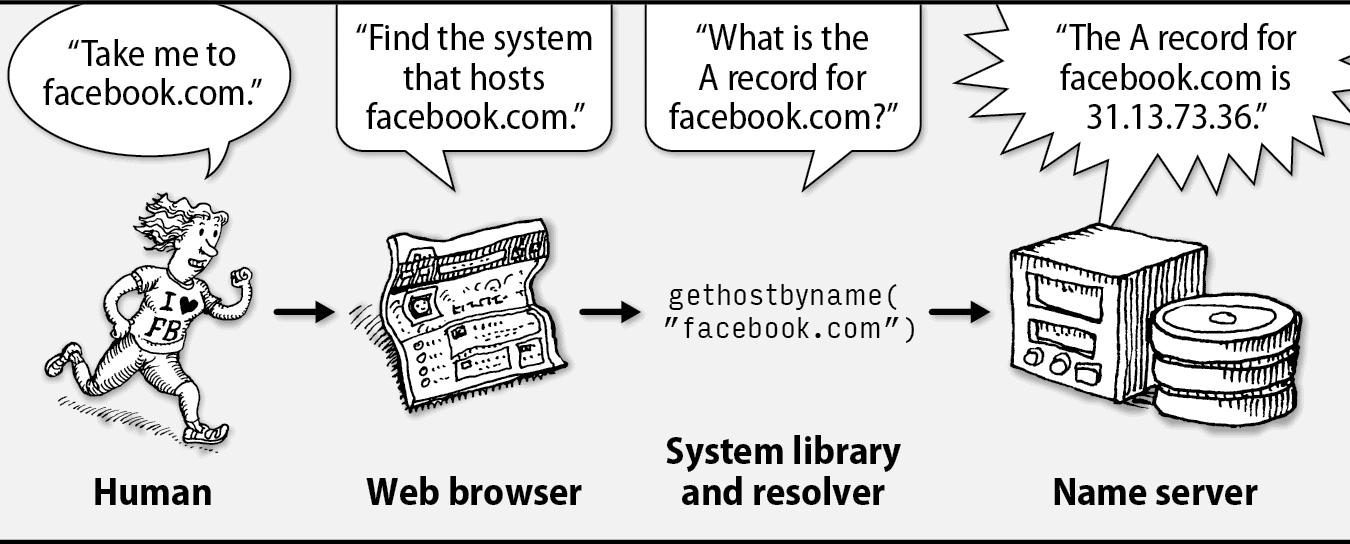
\includegraphics{images/00621.gif}

First, a human types the name of a desired site into a web browser. The
browser then calls the DNS ``resolver'' library to look up the
corresponding address. The resolver library constructs a query for an A
record and sends it to a name server, which returns the A record in its
response. Finally, the browser opens a TCP connection to the target host
through the IP address returned by the name server.


\subsection{DNS service providers}

Years ago, one of the core tasks of every system administrator was to set up and maintain a DNS server for their organization.
Today, the landscape has changed.
If an organization maintains a DNS server at all, it is frequently for internal use only.

Microsoft's Active Directory system includes an integrated DNS server that meshes nicely with the other Microsoft-flavored services found in corporate environments.
However, Active Directory is suitable only for internal use.
It should never be used as an external (Internet-facing) DNS server because of potential security concerns.

Every organization still needs an external-facing DNS server, but it's now common to use one of the many commercial ``managed'' DNS providers for this function.
These services offer a GUI management interface and highly available, secure DNS infrastructure for only pennies (or dollars) a day.
Amazon Route 53, CloudFlare, GoDaddy, DNS Made Easy, and Rackspace are just a few of the major providers.

Of course, you can still set up and maintain your own DNS server
(internal or external) if you wish. You have dozens of DNS
implementations to choose from, but the Berkeley Internet Name Domain (BIND) system still dominates the Internet.
Over 75 percent of DNS servers run some form of it, according to the July, 2015 ISC Internet Domain Survey.

Regardless of which path you choose, as a system administrator you need to understand the basic concepts and architecture of DNS.
The first few sections of this chapter focus on that important foundational knowledge.
Starting on this page, we show some specific configurations for BIND.


\section{DNS for lookups}

Regardless of whether you run your own name server, use a managed DNS service, or have someone else providing DNS service for you, you'll certainly want
to configure all of your systems to look up names in DNS.

Two steps are needed to make this happen. First, you configure your
systems as DNS clients. Second, you tell the systems when to use DNS as
opposed to other name lookup methods such as a static {/etc/hosts} file.


\subsection{resolv.conf: client resolver configuration}

Each host on the network should be a DNS client.
You configure the client-side resolver in the file /etc/resolv.conf.
This file lists the name servers to which the host can send queries.

See \cref{chap:dhcp} for more information about DHCP.

If your host gets its IP address and network parameters from a DHCP
server, the {/etc/resolv.conf} file is normally set up for you
automatically. Otherwise, you must edit the file by hand. The format is

%\includegraphics{images/00622.gif}

Up to three name servers can be listed. Here's a complete
example:\protect\hypertarget{part0024_split_005.htmlux5cux23_idIndexMarker1979}{}{}\protect\hypertarget{part0024_split_005.htmlux5cux23_idIndexMarker1980}{}{}

%\includegraphics{images/00623.gif}

The {search} line lists the domains to query if a hostname is not fully
qualified. For example, if a user issues the command {ssh} {coraline},
the resolver completes the name with the first domain in the search list
and looks for coraline.atrust.com. If no such name exists, the resolver
also tries coraline.booklab.atrust.com. The number of domains that can
be specified in a {search} directive is resolver-specific; most allow
between six and eight, with a limit of 256 characters.

The name servers listed in {resolv.conf} must be configured to allow
your host to submit queries. They must also be recursive; that is, they
must answer queries to the best of their ability and not try to refer
you to other name servers; see
\protect\hyperlink{part0024_split_013.htmlux5cux23_idTextAnchor857}{this
page}.

DNS servers are contacted in order. As long as the first one continues
to answer queries, the others are ignored. If a problem occurs, the
query eventually times out and the next name server is tried. Each
server is tried in turn, up to four times. The timeout interval
increases with each failure. The default timeout interval is five
seconds, which seems like forever to impatient users.

\protect\hypertarget{part0024_split_006.html}{}{}

\hypertarget{part0024_split_006.htmlux5cux23_idContainer1069}{}
\hypertarget{part0024_split_006.htmlux5cux23calibre_pb_5}{%
\subsection[: who do I ask for a
name?]{\texorpdfstring{{\protect\hypertarget{part0024_split_006.htmlux5cux23_idTextAnchor848}{}{}nsswitch.conf}:
who do I ask for a
name?}{nsswitch.conf: who do I ask for a name?}}\label{part0024_split_006.htmlux5cux23calibre_pb_5}}

\protect\hypertarget{part0024_split_006.htmlux5cux23_idIndexMarker1981}{}{}Both
FreeBSD and Linux use a switch file,
\protect\hypertarget{part0024_split_006.htmlux5cux23_idIndexMarker1982}{}{}\protect\hypertarget{part0024_split_006.htmlux5cux23_idIndexMarker1983}{}{}{/etc/nsswitch.conf,}
to specify how hostname-to-IP-address mappings should be performed and
whether DNS should be tried first, last, or not at all. If no switch
file is present, the default behavior is

%\includegraphics{images/00624.gif}

The {!UNAVAIL} clause means that if DNS is available but a name is not
found there, the lookup attempt should fail rather than continuing to
the next entry (in this case, the {/etc/hosts} file). If no name server
is running (as might be the case during boot), the lookup process does
consult the {hosts} file.

Our example distributions all provide the following default
{nsswitch.conf} entry:

%\includegraphics{images/00625.gif}

This configuration gives precedence to the {/etc/hosts} file, which is
always checked. DNS is consulted only for names that are unresolvable
through {/etc/hosts}.

There is really no best way to configure lookups---it depends on how
your site is managed. In general, we prefer to keep as much host
information as possible in DNS but always preserve the ability to fall
back to the static {hosts} file during the boot process if necessary.

If name service is provided for you by an outside organization, you
might be done with DNS configuration after setting up {resolv.conf} and
{nsswitch.conf}. If so, you can skip the rest of this chapter, or read
on to learn more.




\section{The DNS namespace}

\protect\hypertarget{part0024_split_007.htmlux5cux23_idIndexMarker1984}{}{}The
DNS namespace is organized into a tree that contains both
\protect\hypertarget{part0024_split_007.htmlux5cux23_idIndexMarker1985}{}{}forward
mappings and
\protect\hypertarget{part0024_split_007.htmlux5cux23_idIndexMarker1986}{}{}reverse
mappings. Forward mappings map hostnames to IP addresses (and other
records), and reverse mappings map IP addresses to hostnames. Every
complete hostname (e.g., nubark.atrust.com) is a node in the forward
branch of the tree, and (in theory) every IP address is a node in the
reverse branch.
\protect\hyperlink{part0024_split_007.htmlux5cux23_idTextAnchor850}{Exhibit
B} shows the general layout of the naming tree.

\paragraph[{Exhibit B: }DNS zone tree]{\texorpdfstring{{Exhibit B:
}\protect\hypertarget{part0024_split_007.htmlux5cux23_idTextAnchor850}{}{}DNS
zone tree}{Exhibit B: DNS zone tree}}

%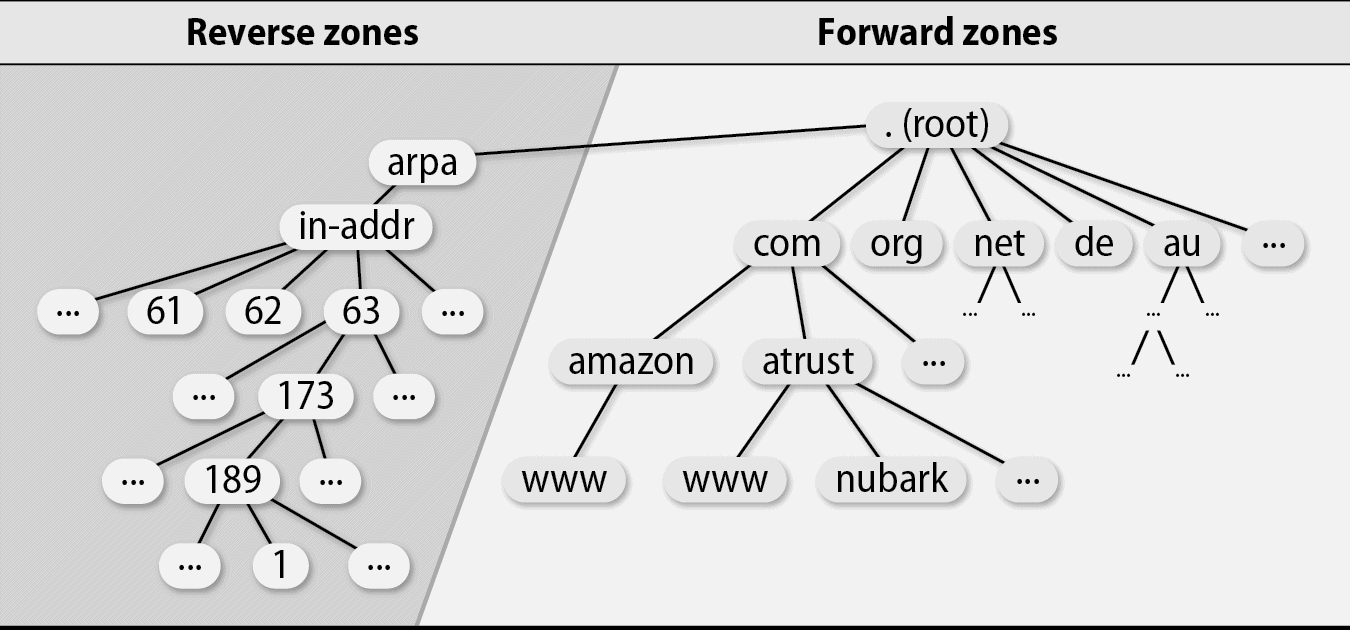
\includegraphics{images/00626.gif}

\protect\hypertarget{part0024_split_007.htmlux5cux23_idIndexMarker1987}{}{}\protect\hypertarget{part0024_split_007.htmlux5cux23_idIndexMarker1988}{}{}\protect\hypertarget{part0024_split_007.htmlux5cux23_idIndexMarker1989}{}{}\protect\hypertarget{part0024_split_007.htmlux5cux23_idIndexMarker1990}{}{}\protect\hypertarget{part0024_split_007.htmlux5cux23_idIndexMarker1991}{}{}To
allow the same DNS system to manage both names (which have the most
significant information on the right), and IP addresses (which have the
most significant part on the left), the IP branch of the namespace is
inverted by listing the octets of the IP address backwards. For example,
if host nubark.atrust.com has IP address 63.173.189.1, the corresponding
node of the forward branch of the naming tree is ``nubark.atrust.com.''
and the node of the
\protect\hypertarget{part0024_split_007.htmlux5cux23_idIndexMarker1992}{}{}reverse
branch is
``1.189.173.63.\protect\hypertarget{part0024_split_007.htmlux5cux23_idIndexMarker1993}{}{}\protect\hypertarget{part0024_split_007.htmlux5cux23_idIndexMarker1994}{}{}in-addr.arpa.''.
The in-addr.arpa portion of the name is a fixed suffix.

\protect\hypertarget{part0024_split_007.htmlux5cux23_idIndexMarker1995}{}{}\protect\hypertarget{part0024_split_007.htmlux5cux23_idIndexMarker1996}{}{}\protect\hypertarget{part0024_split_007.htmlux5cux23_idIndexMarker1997}{}{}Both
of these names end with a dot, just as the full pathnames of files
always start with a slash. That makes them ``fully qualified domain
names'' or FQDNs for short. Outside the context of DNS, names like
nubark.atrust.com (without the final dot) are sometimes referred to as
``fully qualified hostnames,'' but this is a {colloquialism}. Within the
DNS system itself, the presence or absence of the trailing dot is of
crucial importance.

\protect\hypertarget{part0024_split_007.htmlux5cux23_idIndexMarker1998}{}{}Two
types of top-level domains exist:
\protect\hypertarget{part0024_split_007.htmlux5cux23_idIndexMarker1999}{}{}\protect\hypertarget{part0024_split_007.htmlux5cux23_idIndexMarker2000}{}{}country
code domains (ccTLDs) and
\protect\hypertarget{part0024_split_007.htmlux5cux23_idIndexMarker2001}{}{}\protect\hypertarget{part0024_split_007.htmlux5cux23_idIndexMarker2002}{}{}generic
top-level domains (gTLDs).
\protect\hypertarget{part0024_split_007.htmlux5cux23_idIndexMarker2003}{}{}ICANN,
the
\protect\hypertarget{part0024_split_007.htmlux5cux23_idIndexMarker2004}{}{}Internet
Corporation for Assigned Names and Numbers, accredits various agencies
to be part of its shared registry project for registering names in the
gTLDs such as com, net, and org. To register for a ccTLD name, check the
\protect\hypertarget{part0024_split_007.htmlux5cux23_idIndexMarker2005}{}{}IANA
(\protect\hypertarget{part0024_split_007.htmlux5cux23_idIndexMarker2006}{}{}Internet
Assigned Numbers Authority) web page
{\href{http://iana.org/cctld}{iana.org/cctld}} to find the registry in
charge of a particular country's registration.

\protect\hypertarget{part0024_split_008.html}{}{}

\hypertarget{part0024_split_008.htmlux5cux23_idContainer1069}{}
\hypertarget{part0024_split_008.htmlux5cux23calibre_pb_7}{%
\subsection[Registering a domain
name]{\texorpdfstring{\protect\hypertarget{part0024_split_008.htmlux5cux23_idTextAnchor851}{}{}Registering
a domain
name}{Registering a domain name}}\label{part0024_split_008.htmlux5cux23calibre_pb_7}}

\protect\hypertarget{part0024_split_008.htmlux5cux23_idIndexMarker2007}{}{}To
obtain a
\protect\hypertarget{part0024_split_008.htmlux5cux23_idIndexMarker2008}{}{}\protect\hypertarget{part0024_split_008.htmlux5cux23_idIndexMarker2009}{}{}second-level
domain name (such as blazedgoat.com), you must apply to a registrar for
the appropriate top-level domain. To complete the domain registration
forms, you must choose a name that is not already taken and identify a
technical contact person, an administrative contact person, and at least
two hosts that will be name servers for your domain. Fees vary among
registrars, but these days they are all generally quite inexpensive.

\protect\hypertarget{part0024_split_009.html}{}{}

\hypertarget{part0024_split_009.htmlux5cux23_idContainer1069}{}
\hypertarget{part0024_split_009.htmlux5cux23calibre_pb_8}{%
\subsection[Creating your own
subdomains]{\texorpdfstring{\protect\hypertarget{part0024_split_009.htmlux5cux23_idTextAnchor852}{}{}Creating
your own
subdomains}{Creating your own subdomains}}\label{part0024_split_009.htmlux5cux23calibre_pb_8}}

\protect\hypertarget{part0024_split_009.htmlux5cux23_idIndexMarker2010}{}{}\protect\hypertarget{part0024_split_009.htmlux5cux23_idIndexMarker2011}{}{}The
procedure for creating a subdomain is similar to that for creating a
second-level domain, except that the central authority is now local (or
more accurately, within your own organization). Specifically, the steps
are as follows:

\begin{itemize}
\tightlist
\item
  Choose a name that is unique in the local context.
\item
  Identify two or more hosts to be servers for your new domain.
\item
  Coordinate with the administrator of the parent domain.
\end{itemize}

The two-or-more-servers rule is a policy, not a technical requirement.
You make the rules in your own subdomains, so you can get away with a
single server if you want.

Parent domains should check to be sure that a child domain's name
servers are up and running before performing the delegation. If the
servers are not working, a ``lame delegation'' results, and you might
receive nasty email asking you to clean up your DNS act. Lame
delegations are covered in more detail
\protect\hyperlink{part0024_split_072.htmlux5cux23_idTextAnchor966}{here}.




\section{How DNS works}

Name servers around the world work together to answer queries.
Typically, they distribute information maintained by whichever
administrator is closest to the {query} target. Understanding the roles
and relationships of name servers is important both for day-to-day
operations and for debugging.

\protect\hypertarget{part0024_split_011.html}{}{}

\hypertarget{part0024_split_011.htmlux5cux23_idContainer1069}{}
\hypertarget{part0024_split_011.htmlux5cux23calibre_pb_10}{%
\subsection[Name
servers]{\texorpdfstring{\protect\hypertarget{part0024_split_011.htmlux5cux23_idTextAnchor854}{}{}Name
servers}{Name servers}}\label{part0024_split_011.htmlux5cux23calibre_pb_10}}

\protect\hypertarget{part0024_split_011.htmlux5cux23_idIndexMarker2012}{}{}A
name server performs several chores:

\begin{itemize}
\tightlist
\item
  It answers queries about your site's hostnames and IP addresses.
\item
  It asks about both local and remote hosts on behalf of your users.
\item
  It caches the answers to queries so that it can answer faster next
  time.
\item
  It communicates with other local name servers to keep DNS data
  synchronized.
\end{itemize}

Name servers deal with ``zones,'' where a zone is essentially a domain
minus its subdomains. You will often see the term ``domain'' used where
a zone is what's actually meant, even in this book.

Name servers can operate in several different modes. The distinctions
among them fall along several axes, so the final categorization is often
not tidy. To make things even more confusing, a single server can play
different roles with respect to different zones.
\protect\hyperlink{part0024_split_011.htmlux5cux23_idTextAnchor855}{Table
16.1} lists some of the adjectives used to describe name servers.

\paragraph[{Table 16.1: }Name server taxonomy]{\texorpdfstring{{Table
16.1:
}\protect\hypertarget{part0024_split_011.htmlux5cux23_idIndexMarker2013}{}{}\protect\hypertarget{part0024_split_011.htmlux5cux23_idTextAnchor855}{}{}Name
server
taxonomy\protect\hypertarget{part0024_split_011.htmlux5cux23_idIndexMarker2014}{}{}\protect\hypertarget{part0024_split_011.htmlux5cux23_idIndexMarker2015}{}{}\protect\hypertarget{part0024_split_011.htmlux5cux23_idIndexMarker2016}{}{}\protect\hypertarget{part0024_split_011.htmlux5cux23_idIndexMarker2017}{}{}\protect\hypertarget{part0024_split_011.htmlux5cux23_idIndexMarker2018}{}{}\protect\hypertarget{part0024_split_011.htmlux5cux23_idIndexMarker2019}{}{}\protect\hypertarget{part0024_split_011.htmlux5cux23_idIndexMarker2020}{}{}\protect\hypertarget{part0024_split_011.htmlux5cux23_idIndexMarker2021}{}{}\protect\hypertarget{part0024_split_011.htmlux5cux23_idIndexMarker2022}{}{}\protect\hypertarget{part0024_split_011.htmlux5cux23_idIndexMarker2023}{}{}\protect\hypertarget{part0024_split_011.htmlux5cux23_idIndexMarker2024}{}{}\protect\hypertarget{part0024_split_011.htmlux5cux23_idIndexMarker2025}{}{}}{Table 16.1: Name server taxonomy}}

%\includegraphics{images/00627.gif}

These categorizations vary according to the name server's source of data
(authoritative, caching, master, slave), the type of data saved (stub),
the query path (forwarder), the completeness of answers handed out
(recursive, nonrecursive), and finally, the visibility of the server
(distribution). The next few sections provide additional details on the
most important of these distinctions; the others are described elsewhere
in this chapter.

\protect\hypertarget{part0024_split_012.html}{}{}

\hypertarget{part0024_split_012.htmlux5cux23_idContainer1069}{}
\hypertarget{part0024_split_012.htmlux5cux23calibre_pb_11}{%
\subsection[Authoritative and caching-only
servers]{\texorpdfstring{\protect\hypertarget{part0024_split_012.htmlux5cux23_idTextAnchor856}{}{}Authoritative
and caching-only
servers}{Authoritative and caching-only servers}}\label{part0024_split_012.htmlux5cux23calibre_pb_11}}

\protect\hypertarget{part0024_split_012.htmlux5cux23_idIndexMarker2026}{}{}\protect\hypertarget{part0024_split_012.htmlux5cux23_idIndexMarker2027}{}{}Master,
slave, and caching-only servers are distinguished by two
characteristics: where the data comes from, and whether the server is
authoritative for the domain. Each zone typically has one master name
server. The master server keeps the official copy of the zone's data on
disk. The system administrator changes the zone's data by editing the
master server's data files.

Some sites use multiple masters or even no masters. However, these are
unusual configurations. We describe only the single-master case.

\leavevmode\hypertarget{part0024_split_012.htmlux5cux23_idContainer914}{}%
See
\protect\hyperlink{part0024_split_051.htmlux5cux23_idTextAnchor927}{this
page} for more information about zone transfers.

A slave server gets its data from the master server through a ``zone
transfer'' operation. A zone can have several slave name servers and
{must} have at least one. A stub server is a special kind of slave that
loads only the NS (name server) records from the master. It's fine for
the same machine to be both a master server for some zones and a slave
server for other zones.

A
\protect\hypertarget{part0024_split_012.htmlux5cux23_idIndexMarker2028}{}{}caching-only
name server loads the addresses of the servers for the root domain from
a startup file and accumulates the rest of its data by caching answers
to the queries it resolves.~A caching-only name server has no data of
its own and is not authoritative for any zone (except perhaps the
localhost zone).

An authoritative answer from a name server is ``guaranteed'' to be
accurate; a nonauthoritative answer might be out of date. However, a
very high percentage of nonauthoritative answers are perfectly correct.
Master and slave servers are authoritative for their own zones, but not
for information they may have cached about other domains. Truth be told,
even authoritative answers can be inaccurate if a sysadmin changes the
master server's data but forgets to propagate the changes (e.g., doesn't
change the zone's serial number).

At least one slave server is required for each zone. Ideally, there
should be at least two slaves, one of which is in a location that does
not share common infrastructure with the master. On-site slaves should
live on different networks and different power circuits. When name
service stops, all normal network access stops, too.

\protect\hypertarget{part0024_split_013.html}{}{}

\hypertarget{part0024_split_013.htmlux5cux23_idContainer1069}{}
\hypertarget{part0024_split_013.htmlux5cux23calibre_pb_12}{%
\subsection[Recursive and nonrecursive
servers]{\texorpdfstring{\protect\hypertarget{part0024_split_013.htmlux5cux23_idTextAnchor857}{}{}Recursive
and nonrecursive
servers}{Recursive and nonrecursive servers}}\label{part0024_split_013.htmlux5cux23calibre_pb_12}}

\protect\hypertarget{part0024_split_013.htmlux5cux23_idIndexMarker2029}{}{}\protect\hypertarget{part0024_split_013.htmlux5cux23_idIndexMarker2030}{}{}Name
servers are either recursive or nonrecursive. If a nonrecursive server
has the answer to a query cached from a previous transaction or is
authoritative for the domain to which the query pertains, it provides an
appropriate response. Otherwise, instead of returning a real answer, it
returns a referral to the authoritative servers of another domain that
are more likely to know the answer. A client of a nonrecursive server
must be prepared to accept and act on referrals.

Although nonrecursive servers might seem lazy, they usually have good
reason not to take
\protect\hypertarget{part0024_split_013.htmlux5cux23_idIndexMarker2031}{}{}on
extra work. Authoritative-only servers (e.g.,
\protect\hypertarget{part0024_split_013.htmlux5cux23_idIndexMarker2032}{}{}root
servers and top-level domain servers) are all nonrecursive, but since
they may process tens of thousands of queries per second we can excuse
them for cutting corners.

A recursive server returns only real answers and error messages. It
follows referrals itself, relieving clients of this responsibility. In
other respects, the basic procedure for resolving a query is essentially
the same.

For security, an organization's externally accessible name servers
should always be nonrecursive. Recursive name servers that are visible
to the world can be vulnerable to cache poisoning attacks.

Note well: resolver libraries {do not} understand referrals. Any local
name server listed in a client's {resolv.conf} file must be recursive.

\protect\hypertarget{part0024_split_014.html}{}{}

\hypertarget{part0024_split_014.htmlux5cux23_idContainer1069}{}
\hypertarget{part0024_split_014.htmlux5cux23calibre_pb_13}{%
\subsection[Resource
records]{\texorpdfstring{\protect\hypertarget{part0024_split_014.htmlux5cux23_idTextAnchor858}{}{}\protect\hypertarget{part0024_split_014.htmlux5cux23_idIndexMarker2033}{}{}Resource
records}{Resource records}}\label{part0024_split_014.htmlux5cux23calibre_pb_13}}

Each site maintains one or more pieces of the distributed database that
makes up the world-wide DNS system. Your piece of the database consists
of text files that contain records for each of your hosts; these are
known as ``resource records.'' Each record is a single line consisting
of a name (usually a hostname), a record type, and some data values. The
name field can be omitted if its value is the same as that of the
previous line.

For example, the lines

%\includegraphics{images/00628.gif}

in the ``forward'' file (called {atrust.com}), and the line

%\includegraphics{images/00629.gif}

\leavevmode\hypertarget{part0024_split_014.htmlux5cux23_idContainer917}{}%
See
\protect\hyperlink{part0024_split_027.htmlux5cux23_idTextAnchor882}{this
page} for more information about MX records.

in the
``\protect\hypertarget{part0024_split_014.htmlux5cux23_idIndexMarker2034}{}{}reverse''
file (called {63.173.189.rev}) associate nubark.atrust.com with the IP
address 63.173.189.1. The MX record routes email addressed to this
machine to the host mailserver.atrust.com.

The IN fields denote the record classes. In practice, this field is
always IN for Internet.

Resource records are the lingua franca of DNS and are independent of the
configuration files that control the operation of any given DNS server
implementation. They are also the pieces of data that flow around the
DNS system and become cached at various locations.

\protect\hypertarget{part0024_split_015.html}{}{}

\hypertarget{part0024_split_015.htmlux5cux23_idContainer1069}{}
\hypertarget{part0024_split_015.htmlux5cux23calibre_pb_14}{%
\subsection[Delegation]{\texorpdfstring{\protect\hypertarget{part0024_split_015.htmlux5cux23_idTextAnchor859}{}{}Delegation}{Delegation}}\label{part0024_split_015.htmlux5cux23calibre_pb_14}}

\protect\hypertarget{part0024_split_015.htmlux5cux23_idIndexMarker2035}{}{}All
name servers read the identities of
the\protect\hypertarget{part0024_split_015.htmlux5cux23_idIndexMarker2036}{}{}\protect\hypertarget{part0024_split_015.htmlux5cux23_idIndexMarker2037}{}{}
root servers from a local config file or have them built into the code.
The root servers know the name servers for com, net, edu, fi, de, and
other top-level domains. Farther down the chain, edu knows about
colorado.edu, berkeley.edu, and so on. Each domain can delegate
authority for its subdomains to other servers.

Let's inspect a real example. Suppose we want to look up the address for
the machine vangogh.cs.berkeley.edu from the machine
lair.cs.colorado.edu. The host lair asks its local name server,
ns.cs.colorado.edu, to figure out the answer. The following illustration
(\protect\hyperlink{part0024_split_015.htmlux5cux23_idTextAnchor860}{Exhibit
C}) shows the subsequent events.

\paragraph[{Exhibit C: }DNS query process for
vangogh.cs.berkeley.edu]{\texorpdfstring{{Exhibit C:
}\protect\hypertarget{part0024_split_015.htmlux5cux23_idTextAnchor860}{}{}DNS
query process for
vangogh.cs.berkeley.edu}{Exhibit C: DNS query process for vangogh.cs.berkeley.edu}}

%\includegraphics{images/00630.gif}

The numbers on the arrows between servers show the order of events, and
a letter denotes the type of transaction (query, referral, or answer).
We assume that none of the required information was cached before the
query, except for the names and IP addresses of the servers of the root
domain.

The local server doesn't know vangogh's address. In fact, it doesn't
know anything about cs.berkeley.edu or berkeley.edu or even edu. It does
know servers for the root domain, however, so it queries a root server
about vangogh.cs.berkeley.edu and receives a referral to the servers for
edu.

The local name server is a recursive server. When the answer to a query
consists of a referral to another server, the local server resubmits the
query to the new server. It continues to follow referrals until it finds
a server that has the data it's looking for.

In this case, the local name server sends its query to a server of the
edu domain (asking, as always, about vangogh.cs.berkeley.edu) and gets
back a referral to the servers for berkeley.edu. The local name server
then repeats this same query on a berkeley.edu server. If the Berkeley
server doesn't have the answer cached, it returns a referral to the
servers for cs.berkeley.edu. The cs.berkeley.edu server is authoritative
for the requested information, looks the answer up in its zone files,
and returns vangogh's address.

When the dust settles, ns.cs.colorado.edu has cached vangogh's address.
It has also cached data on the servers for edu, berkeley.edu, and
cs.berkeley.edu.

You can view the query process in detail with {dig +trace} or {drill
-T}. ({dig} and {drill} are DNS query tools: {dig} from the BIND
distribution and {drill} from NLnet Labs.)

\protect\hypertarget{part0024_split_016.html}{}{}

\hypertarget{part0024_split_016.htmlux5cux23_idContainer1069}{}
\hypertarget{part0024_split_016.htmlux5cux23calibre_pb_15}{%
\subsection[Caching and
efficiency]{\texorpdfstring{\protect\hypertarget{part0024_split_016.htmlux5cux23_idTextAnchor861}{}{}Caching
and
efficiency}{Caching and efficiency}}\label{part0024_split_016.htmlux5cux23calibre_pb_15}}

\protect\hypertarget{part0024_split_016.htmlux5cux23_idIndexMarker2038}{}{}\protect\hypertarget{part0024_split_016.htmlux5cux23_idIndexMarker2039}{}{}Caching
increases the efficiency of lookups: a cached answer is almost free and
is usually correct because hostname-to-address mappings change
infrequently. An answer is saved for a period of time called the
``\protect\hypertarget{part0024_split_016.htmlux5cux23_idIndexMarker2040}{}{}\protect\hypertarget{part0024_split_016.htmlux5cux23_idIndexMarker2041}{}{}time
to live'' (TTL), which is specified by the owner of the data record in
question.

Most queries are for local hosts and can be resolved quickly. Users also
inadvertently help with efficiency because they repeat many queries;
after the first instance of a query, the repeats are more or less free.

Under normal conditions, your site's resource records should use a TTL
that is somewhere between an hour and a day. The longer the TTL, the
less network traffic will be consumed by Internet clients obtaining
fresh copies of the record.

If you have a specific service that is load-balanced across logical
subnets (often called ``global server load balancing''), you may be
required by your load-balancing vendor to choose a shorter TTL, such as
10 seconds or 1 minute. The short TTL lets the load balancer react
quickly to inoperative servers and
\protect\hypertarget{part0024_split_016.htmlux5cux23_idIndexMarker2042}{}{}denial
of service attacks. The system still works correctly with short TTLs,
but your name servers have to work hard.

In the vangogh example above, the TTLs were 42 days for the roots, 2
days for edu, 2 days for berkeley.edu, and 1 day for
vangogh.cs.berkeley.edu. These are reasonable values. If you are
planning a massive renumbering, change the TTLs to a shorter value well
before you start.

DNS servers also implement
\protect\hypertarget{part0024_split_016.htmlux5cux23_idIndexMarker2043}{}{}\protect\hypertarget{part0024_split_016.htmlux5cux23_idIndexMarker2044}{}{}negative
caching. That is, they remember when a query fails and do not repeat
that query until the negative caching TTL value has expired. Negative
caching can potentially save answers of the following types:

\begin{itemize}
\tightlist
\item
  No host or domain matches the name queried.
\item
  The type of data requested does not exist for this host.
\item
  The server is not responding.
\item
  The server is unreachable because of network problems.
\end{itemize}

The BIND implementation caches the first two types of negative data and
allows the negative cache times to be configured.

\protect\hypertarget{part0024_split_017.html}{}{}

\hypertarget{part0024_split_017.htmlux5cux23_idContainer1069}{}
\hypertarget{part0024_split_017.htmlux5cux23calibre_pb_16}{%
\subsection[Multiple answers and round robin DNS load
balancing]{\texorpdfstring{\protect\hypertarget{part0024_split_017.htmlux5cux23_idTextAnchor862}{}{}Multiple
answers and round robin DNS load
balancing}{Multiple answers and round robin DNS load balancing}}\label{part0024_split_017.htmlux5cux23calibre_pb_16}}

\protect\hypertarget{part0024_split_017.htmlux5cux23_idIndexMarker2045}{}{}\protect\hypertarget{part0024_split_017.htmlux5cux23_idIndexMarker2046}{}{}A\protect\hypertarget{part0024_split_017.htmlux5cux23_idIndexMarker2047}{}{}
name server often receives multiple records in response to a query. For
example, the response to a query for the name servers of the root domain
would list all 13 servers.

You can take advantage of this balancing effect for your own servers by
assigning several different IP addresses (for different machines) to a
single hostname:

%\includegraphics{images/00631.gif}

Most name servers return multirecord sets in a different order each time
they receive a query, rotating them in round robin fashion. When a
client receives a response with multiple records, the most common
behavior is to try the addresses in the order returned by the DNS
server. However, this behavior is not required. Some clients may behave
differently.

This scheme is commonly referred to as round robin DNS load balancing.
However, it is a crude solution at best. Large sites use load-balancing
software (such as HAProxy; see
\protect\hyperlink{part0027_split_030.htmlux5cux23_idTextAnchor1269}{this
page}) or dedicated load-balancing appliances.

\protect\hypertarget{part0024_split_018.html}{}{}

\hypertarget{part0024_split_018.htmlux5cux23_idContainer1069}{}
\hypertarget{part0024_split_018.htmlux5cux23calibre_pb_17}{%
\subsection[Debugging with query
tools]{\texorpdfstring{\protect\hypertarget{part0024_split_018.htmlux5cux23_idTextAnchor863}{}{}Debugging
with query
tools}{Debugging with query tools}}\label{part0024_split_018.htmlux5cux23calibre_pb_17}}

\leavevmode\hypertarget{part0024_split_018.htmlux5cux23_idContainer920}{}%
See
\protect\hyperlink{part0024_split_059.htmlux5cux23_idTextAnchor938}{this
page} for more information about DNSSEC.

\protect\hypertarget{part0024_split_018.htmlux5cux23_idIndexMarker2048}{}{}Five
command-line tools that query the DNS database are distributed with
BIND:
\protect\hypertarget{part0024_split_018.htmlux5cux23_idIndexMarker2049}{}{}{nslookup},
\protect\hypertarget{part0024_split_018.htmlux5cux23_idIndexMarker2050}{}{}{dig},
\protect\hypertarget{part0024_split_018.htmlux5cux23_idIndexMarker2051}{}{}{host},
\protect\hypertarget{part0024_split_018.htmlux5cux23_idIndexMarker2052}{}{}{drill}
and
\protect\hypertarget{part0024_split_018.htmlux5cux23_idIndexMarker2053}{}{}\protect\hypertarget{part0024_split_018.htmlux5cux23_idIndexMarker2054}{}{}{delv}.{
nslookup} and {host} are simple and have pretty output, but you need
{dig} or {drill} to get all the details. {drill} is better for following
DNSSEC signature chains. The name {drill} is a pun on {dig} (the Domain
Information Groper), implying you can get even more info from DNS with
{drill} than you can with {dig}. {delv} is new to BIND 9.10 and will
eventually replace {drill} for DNSSEC debugging.

\leavevmode\hypertarget{part0024_split_018.htmlux5cux23_idContainer921}{}%
See
\protect\hyperlink{part0024_split_046.htmlux5cux23_idTextAnchor920}{this
page} for more information about split DNS.

By default, {dig} and {drill} query the name servers configured in{
/etc/resolv.conf}. A {@}{nameserver} argument makes either command query
a specific name server. The ability to query a particular server lets
you check to be sure that any changes you make to a zone have been
propagated to secondary servers and to the outside world. This feature
is especially useful if you use views (split DNS) and need to verify
that you have configured them correctly.

If you specify a record type, {dig} and {drill} query for that type
only. The pseudo-type {any} is a bit sneaky: instead of returning all
data associated with a name, it returns all {cached} data associated
with the name. So, to get all records, you might have to do {dig}
{domain} {NS} followed by {dig @ns1.}{domain}{ }{domain}{ any}.
(Authoritative data counts as cached in this context.)

{dig} has about 50 options and {drill} about half that many. Either
command accepts an {-h} flag to list the various options. (You'll
probably want to pipe the output through {less}.) For both tools, {-x}
reverses the bytes of an IP address and does a reverse query. The
{+trace} flag to {dig} or {-T} to {drill} shows the iterative steps in
the resolution process from the roots down.

{dig} and {drill} include the notation {aa} in the output flags if an
answer is authoritative (i.e., it comes directly from a master or slave
server of that zone). The code {ad} indicates that an answer was
authenticated by DNSSEC. When testing a new configuration, be sure that
you look up data for both local and remote hosts. If you can access a
host by IP address but not by name, DNS is probably the culprit.

The most common use of {dig} is to determine what records are currently
being returned for a particular name. If only an {AUTHORITY} response is
returned, you have been referred to another name server. If an {ANSWER}
response is returned, your question has been directly answered (and
other information may be included as well).

It's often useful to follow the delegation chain manually from the root
servers to verify that everything is in the right place. Below we look
at an example of that process for the name www.viawest.com. First, we
query a root server to see who is authoritative for viawest.com by
requesting the start-of-authority (SOA) record:

%\includegraphics{images/00632.gif}

Note that the status returned is
\protect\hypertarget{part0024_split_018.htmlux5cux23_idIndexMarker2055}{}{}{NOERROR}.
That tells us that the query returned a response without notable errors.
Other common status values are
\protect\hypertarget{part0024_split_018.htmlux5cux23_idIndexMarker2056}{}{}{NXDOMAIN},
which indicates the name requested doesn't exist (or isn't registered),
and
\protect\hypertarget{part0024_split_018.htmlux5cux23_idIndexMarker2057}{}{}{SERVFAIL},
which usually indicates a configuration error on the name server itself.

This {AUTHORITY SECTION} tells us that the global top-level domain
(gTLD) servers are the next link in the authority chain for this domain.
So, we pick one at random and repeat the same query:

%\includegraphics{images/00633.gif}

This response is much more succinct, and we now know that the next
server to query is ns1.viawest.com (or ns2.viawest.com).

%\includegraphics{images/00634.gif}

This query returns an {ANSWER} for the viawest.com domain. We now know
an authoritative name server and can query for the name we actually
want, www.viawest.com.

%\includegraphics{images/00635.gif}

This final query shows us that www.viawest.com has a CNAME record
pointed at hm-d8ebfa-via1.threatx.io, meaning that it is another name
for the threatx host (a host operated by a cloud-based distributed
denial-of-service provider).

Of course, if you query a recursive name server, it will follow the
entire delegation chain on your behalf. But when debugging, it's
typically more useful to investigate the chain link by link.



\section{The DNS database}

{\protect\hypertarget{part0024_split_019.htmlux5cux23_idIndexMarker2058}{}{}}A
zone's DNS database is a set of text files maintained by the system
administrator on the zone's master name server. These text files are
often called zone files. They contain two types of entries: parser
commands (things like {\$ORIGIN} and
\protect\hypertarget{part0024_split_019.htmlux5cux23_idIndexMarker2059}{}{}{\$TTL})
and resource records. Only the resource records are really part of the
database; the parser commands just provide some shorthand ways to enter
records.

\protect\hypertarget{part0024_split_020.html}{}{}

\hypertarget{part0024_split_020.htmlux5cux23_idContainer1069}{}
\hypertarget{part0024_split_020.htmlux5cux23calibre_pb_19}{%
\subsection[Parser commands in zone
files]{\texorpdfstring{\protect\hypertarget{part0024_split_020.htmlux5cux23_idTextAnchor866}{}{}Parser
commands in zone
files}{Parser commands in zone files}}\label{part0024_split_020.htmlux5cux23calibre_pb_19}}

\leavevmode\hypertarget{part0024_split_020.htmlux5cux23_idContainer926}{}%
Zone file commands are standardized in RFCs 1035 and 2308.

Commands can be embedded in zone files to make the zone files more
readable and easier to maintain. The commands either influence the way
the parser interprets subsequent records or they expand into multiple
DNS records themselves. Once a zone file has been read and interpreted,
none of these commands remain a part of the zone's data (at least, not
in their original forms).

\protect\hypertarget{part0024_split_020.htmlux5cux23_idTextAnchor867}{}{}Three
commands ({\$ORIGIN}, {\$INCLUDE}, and {\$TTL}) are standard for all DNS
implementations, and a fourth, {\$GENERATE}, is found only in BIND.
Commands must start in column one and occur on a line by themselves.

Zone files are read and parsed from top to bottom in a single pass. As
the name server reads a zone file, it adds the default domain (or
``origin'') to any names that are not already fully qualified. The
origin defaults to the domain name specified in the name server's
configuration file. However, you can set the origin or change it within
a zone file by using
the\protect\hypertarget{part0024_split_020.htmlux5cux23_idIndexMarker2060}{}{}
{\$ORIGIN} directive:

%\includegraphics{images/00636.gif}

The use of relative names where fully qualified names are expected saves
lots of typing and makes zone files much easier to read.

Many sites use the {\$INCLUDE} directive in their zone database files to
separate overhead records from data records, to separate logical pieces
of a zone file, or to keep cryptographic keys in a file with restricted
permissions. The syntax is

%\includegraphics{images/00637.gif}

The specified file is read into the database at the point of the
\protect\hypertarget{part0024_split_020.htmlux5cux23_idIndexMarker2061}{}{}{\$INCLUDE}
directive. If {filename} is not an absolute path, it is interpreted
relative to the home directory of the running name server.

If you supply an {origin} value, the parser acts as if an {\$ORIGIN}
directive precedes the contents of the file being read. Watch out: the
origin does not revert to its previous value after the {\$INCLUDE} has
been executed. You'll probably want to reset the origin, either at the
end of the included file or on the line following the {\$INCLUDE}
statement.

\protect\hypertarget{part0024_split_020.htmlux5cux23_idTextAnchor868}{}{}The
\protect\hypertarget{part0024_split_020.htmlux5cux23_idIndexMarker2062}{}{}{\$TTL}
directive sets a default value for the time-to-live field of the records
that follow it. It must be the first line of the zone file. The default
units for the {\$TTL} value are seconds, but you can also qualify
numbers with {h} for hours, {m} for minutes, {d} for days, or {w} for
weeks. For example, the lines

%\includegraphics{images/00638.gif}

all set the {\$TTL} to one day.

\protect\hypertarget{part0024_split_021.html}{}{}

\hypertarget{part0024_split_021.htmlux5cux23_idContainer1069}{}
\hypertarget{part0024_split_021.htmlux5cux23calibre_pb_20}{%
\subsection[Resource
records]{\texorpdfstring{\protect\hypertarget{part0024_split_021.htmlux5cux23_idTextAnchor869}{}{}\protect\hypertarget{part0024_split_021.htmlux5cux23_idIndexMarker2063}{}{}Resource
records}{Resource records}}\label{part0024_split_021.htmlux5cux23calibre_pb_20}}

Each zone of the DNS hierarchy has a set of resource records associated
with it. The basic format of a resource record is

%\includegraphics{images/00639.gif}

Fields are separated by whitespace (tabs or spaces) and can contain the
special characters shown in
\protect\hyperlink{part0024_split_021.htmlux5cux23_idTextAnchor870}{Table
16.2}.

\paragraph[{Table 16.2: }Special characters in resource
records]{\texorpdfstring{{Table 16.2:
}\protect\hypertarget{part0024_split_021.htmlux5cux23_idIndexMarker2064}{}{}\protect\hypertarget{part0024_split_021.htmlux5cux23_idTextAnchor870}{}{}Special
characters in resource
records}{Table 16.2: Special characters in resource records}}

%\includegraphics{images/00640.gif}

The {name} field identifies the entity (usually a host or domain) that
the record describes. If several consecutive records refer to the same
entity, the name can be omitted after the first record as long as the
subsequent records begin with white-space. If present, the {name} field
must begin in column one.

A name can be either relative or absolute. Absolute names end with a dot
and are complete. Internally, the software deals only with absolute
names; it appends the current origin and a dot to any name that does not
already end in a dot. This feature allows names to be shorter, but it
also invites mistakes.

For example, if cs.colorado.edu were the current domain, the name
``anchor'' would be interpreted as ``anchor.cs.colorado.edu.''. If by
mistake you entered the name as ``anchor.cs.colorado.edu'', the lack of
a final dot would still imply a relative name, resulting in the name
``anchor.cs.colorado.edu.cs.colorado.edu.'' This kind of mistake is
common.

\protect\hypertarget{part0024_split_021.htmlux5cux23_idTextAnchor871}{}{}The{
ttl} (time to live) field specifies the length of time, in seconds, that
the record can be cached and still be considered valid. It is often
omitted, except in the root server hints file. It defaults to the value
set by the {\$TTL} directive, which must be the first line of the zone
data file.

Increasing the value of the {ttl} parameter to about a week
substantially reduces network traffic and DNS load. However, once
records have been cached outside your local network, you cannot force
them to be discarded. If you plan a massive renumbering and your old
{ttl} was a week, lower the {\$TTL} value (e.g., to one hour) at least a
week before your intended renumbering. This preparatory step makes sure
that records with week-long {ttl}s are expired and replaced with records
that have one-hour {ttl}s. You can then be certain that all your updates
will propagate together within an hour. Set the {ttl}s back to their
original value after you've completed your update campaign.

Some sites set the TTL on the records for Internet-facing servers to a
low value so that if a server experiences problems (network failure,
hardware failure,
\protect\hypertarget{part0024_split_021.htmlux5cux23_idIndexMarker2065}{}{}{denial}-of-{service}
attack, etc.), the administrators can respond by changing the server's
name-to-IP-address mapping. Because the original TTLs were low, the new
values will propagate quickly. For example, the name google.com has a
five-minute TTL, but Google's name servers have a TTL of four days
(345,600 seconds):

%\includegraphics{images/00641.gif}

We used {dig} to obtain these records; we truncated the output.

The {class} specifies the network type. IN for Internet is the default.

Many different types of DNS records are defined, but fewer than 10 are
in common use; IPv6 adds a few more. We divide the resource records into
four groups:

\begin{itemize}
\tightlist
\item
  Zone infrastructure records, which identify domains and their name
  servers
\item
  Basic records, which map between names and addresses and route mail
\item
  Security records, which add authentication and signatures to zone
  files
\item
  Optional records, which provide extra information about hosts or
  domains
\end{itemize}

The contents of the {data} field depend on the record type. A DNS query
for a particular domain and record type returns all matching resource
records from the zone file.
\protect\hyperlink{part0024_split_021.htmlux5cux23_idTextAnchor872}{Table
16.3} lists the common record types.

\paragraph[{Table 16.3: }DNS record types]{\texorpdfstring{{Table 16.3:
}\protect\hypertarget{part0024_split_021.htmlux5cux23_idIndexMarker2066}{}{}\protect\hypertarget{part0024_split_021.htmlux5cux23_idIndexMarker2067}{}{}\protect\hypertarget{part0024_split_021.htmlux5cux23_idTextAnchor872}{}{}DNS
record types}{Table 16.3: DNS record types}}

%\includegraphics{images/00642.gif}

Some record types are obsolete, experimental, or not widely used. See
your name server's implementation documentation for a complete list.
Most records are maintained by hand (by editing text files or by
entering them in a web GUI), but the security resource records require
cryptographic processing and so must be managed with software tools.
These records are described in the DNSSEC section beginning
\protect\hyperlink{part0024_split_059.htmlux5cux23_idTextAnchor938}{here}.

The order of resource records in the zone file is arbitrary, but
traditionally the SOA record is first, followed by the NS records. The
records for each host are usually kept together. It's common practice to
sort by the {name} field, although some sites sort by IP address so that
it's easier to identify unused addresses.

As we describe each type of resource record in detail in the next
sections, we inspect some sample records from the atrust.com domain's
data files. The default domain in this context is ``atrust.com.'', so a
host specified as ``bark'' really means ``bark.atrust.com.''.

\leavevmode\hypertarget{part0024_split_021.htmlux5cux23_idContainer934}{}%
See
\protect\hyperlink{part0021_split_003.htmlux5cux23_idTextAnchor618}{this
page} for more information about RFCs.

The format and interpretation of each type of resource record is
specified by the IETF in the RFC series. In the upcoming sections, we
list the specific RFCs relevant to each record type (along with their
years of origin) in a margin note.

\protect\hypertarget{part0024_split_022.html}{}{}

\hypertarget{part0024_split_022.htmlux5cux23_idContainer1069}{}
\hypertarget{part0024_split_022.htmlux5cux23calibre_pb_21}{%
\subsection[The SOA
record]{\texorpdfstring{\protect\hypertarget{part0024_split_022.htmlux5cux23_idTextAnchor873}{}{}The
SOA
record}{The SOA record}}\label{part0024_split_022.htmlux5cux23calibre_pb_21}}

\leavevmode\hypertarget{part0024_split_022.htmlux5cux23_idContainer935}{}%
SOA records are specified in RFC1035 (1987).

An
\protect\hypertarget{part0024_split_022.htmlux5cux23_idIndexMarker2068}{}{}\protect\hypertarget{part0024_split_022.htmlux5cux23_idIndexMarker2069}{}{}SOA
(Start of Authority) record marks the beginning of a zone, a group of
resource records located at the same place within the DNS namespace. The
data for a DNS domain usually includes at least two zones: one for
translating hostnames to IP addresses, called the forward zone, and
others that map IP addresses back to hostnames, called reverse zones.

Each zone has exactly one SOA record. The SOA record includes the name
of the zone, the primary name server for the zone, a technical contact,
and various timeout values. Comments are introduced by a semicolon.
Here's an example:

%\includegraphics{images/00643.gif}

The {name} field of the SOA record (atrust.com. in this example) often
contains the symbol {@}, which is shorthand for the name of the current
zone. The value of {@} is the domain name specified in the {zone}
statement of {named.conf}. This value can be changed from within the
zone file with the {\$ORIGIN} parser directive (see
\protect\hyperlink{part0024_split_020.htmlux5cux23_idTextAnchor867}{this
page}).

This example has no {ttl} field. The class is IN for Internet, the type
is SOA, and the remaining items form the {data} field. The numerical
parameters in parentheses are timeout values and are often written on
one line without comments.

``ns1.atrust.com.'' is the zone's master name server. Actually, any name
server for the zone can be listed in the SOA record unless you are using
dynamic DNS. In that case, the SOA record must name the master server.

``hostmaster.atrust.com.'' was originally intended to be the email
address of the technical contact in the format ``{user.host.}'' rather
than the standard {user@host.} Unfortunately, due to spam concerns and
other reasons, most sites do not keep this contact info updated.

The parentheses continue the SOA record over several lines.

The first numeric parameter is the serial number of the zone's
configuration data. The serial number is used by slave servers to
determine when to get fresh data. It can be any 32-bit integer and
should be incremented every time the data file for the zone is changed.
Many sites encode the file's modification date in the serial number. For
example, 2017110200 would be the first change to the zone on November 2,
2017.

Serial numbers need not be continuous, but they must increase
monotonically. If by accident you set a really large value on the master
server and that value is transferred to the slaves, then correcting the
serial number on the master will not work. The slaves request new data
only if the master's serial number is larger than theirs.

You can fix this problem in two ways:

\begin{itemize}
\tightlist
\item
  One fix is to exploit the properties of the sequence space in which
  the serial numbers live. This procedure involves adding a large value
  (2{31}) to the bloated serial number, letting all the slave servers
  transfer the data, and then setting the serial number to just what you
  want. This weird arithmetic, with explicit examples, is covered in
  detail in the O'Reilly book titled {DNS and BIND}; RFC1982 describes
  the sequence space.
\item
  A sneaky but more tedious way to fix the problem is to change the
  serial number on the master, kill the slave servers, remove the
  slaves' backup data files so they are forced to reload from the
  master, and restart the slaves. It does not work to just remove the
  files and reload; you must kill and restart the slave servers. This
  method gets hard if you follow best-practices advice and have your
  slave servers geographically distributed, especially if you are not
  the sysadmin for those slave servers.
\end{itemize}

It's a common mistake to change the data files but forget to update the
serial number. Your name server will punish you by failing to propagate
your changes to slave servers.

The next four entries in the SOA record are timeout values, in seconds,
that control how long data can be cached at various points throughout
the world-wide DNS database. Times can also be expressed in units of
minutes, hours, days, or weeks by addition of a suffix of {m}, {h}, {d},
or {w}, respectively. For example, {1h30m} means 1 hour and 30 minutes.
Timeout values represent a tradeoff between efficiency (it's cheaper to
use an old value than to fetch a new one) and accuracy (new values are
more accurate). The four timeout fields are called {refresh}, {update},
{expire}, and {minimum}.

The {refresh} timeout specifies how often slave servers should check
with the master to see if the serial number of the zone's configuration
has changed. Whenever the zone changes, slaves must update their copy of
the zone's data. The slave compares the serial numbers; if the master's
serial number is larger, the slave requests a zone transfer to update
the data. Common values for the {refresh} timeout range from one to six
hours (3,600 to 21,600 seconds).

Instead of just waiting passively for slave servers to time out, master
servers for BIND notify their slaves every time a zone changes. However,
it's possible for an update notification to be lost because of network
congestion, so the refresh timeout should still be set to a reasonable
value.

If a slave server tries to check the master's serial number but the
master does not respond, the slave tries again after the {retry} timeout
period has elapsed. Our experience suggests that 20--60 minutes
(1,200--3,600 seconds) is a good value.

If a master server is down for a long time, slaves will try to refresh
their data many times but always fail. Each slave should eventually
decide that the master is never coming back and that its data is surely
out of date. The {expire} parameter determines how long the slaves will
continue to serve the domain's data authoritatively in the absence of a
master. The system should be able to survive if the master server is
down for a few days, so this parameter should have a longish value. We
recommend a month or two.

The {minimum} parameter in the SOA record sets the time to live for
negative answers that are cached. The default for positive answers
(i.e., actual records) is specified at the top of the zone file with the
{\$TTL} directive. Experience suggests values of several hours to a few
days for {\$TTL} and an hour to a few hours for the {minimum}. BIND
silently discards any {minimum} values greater than 3 hours.

The {\$TTL}, {expire}, and {minimum} parameters eventually force
everyone that uses DNS to discard old data values. The initial design of
DNS relied on the fact that host data was relatively stable and did not
change often. However, DHCP, mobile hosts, and the Internet explosion
have changed the rules. Name servers are desperately trying to cope with
the dynamic update and incremental zone transfer mechanisms described
later.

\protect\hypertarget{part0024_split_023.html}{}{}

\hypertarget{part0024_split_023.htmlux5cux23_idContainer1069}{}
\hypertarget{part0024_split_023.htmlux5cux23calibre_pb_22}{%
\subsection[NS
records]{\texorpdfstring{\protect\hypertarget{part0024_split_023.htmlux5cux23_idTextAnchor874}{}{}\protect\hypertarget{part0024_split_023.htmlux5cux23_idIndexMarker2070}{}{}NS
records}{NS records}}\label{part0024_split_023.htmlux5cux23calibre_pb_22}}

\leavevmode\hypertarget{part0024_split_023.htmlux5cux23_idContainer937}{}%
NS records are specified in RFC1035 (1987).

NS (name server) records
\protect\hypertarget{part0024_split_023.htmlux5cux23_idIndexMarker2071}{}{}identify
the servers that are authoritative for a zone (that is, all the master
and slave servers) and delegate subdomains to other organizations. NS
records are usually placed directly after a zone's SOA record.

The format is

%\includegraphics{images/00644.gif}

For example:

%\includegraphics{images/00645.gif}

The first two lines define name servers for the atrust.com domain. No
{name} is listed because it is the same as the {name} field of the SOA
record that precedes the records; the {name} can therefore be left
blank. The {class} is also not listed because IN is the default and does
not need to be stated explicitly.

The third and fourth lines delegate a subdomain called
booklab.atrust.com to the name servers ubuntu.booklab.atrust.com and
ns1.atrust.com. These records are actually part of the booklab
subdomain, but they must also appear in the parent zone, atrust.com, in
order for the delegation to work. In a similar fashion, NS records for
atrust.com are stored in the .com zone file to define the atrust.com
subdomain and identify its servers. The .com servers refer queries about
hosts in atrust.com to the servers listed in NS records for atrust.com
within the .com domain.

\leavevmode\hypertarget{part0024_split_023.htmlux5cux23_idContainer940}{}%
See
\protect\hyperlink{part0024_split_015.htmlux5cux23_idTextAnchor859}{this
page} for more information about delegation.

The list of name servers in the parent zone should be kept up to date
with those in the zone itself, if possible. Nonexistent servers listed
in the parent zone can delay name service, although clients will
eventually stumble onto one of the functioning name servers. If none of
the name servers listed in the parent exist in the child, a so-called
lame delegation results; see
\protect\hyperlink{part0024_split_072.htmlux5cux23_idTextAnchor966}{this
page}.

Extra servers in the child are OK as long as at least one of the child's
servers still has an NS record in the parent. Check your delegations
occasionally with {dig} or {drill} to be sure they specify an
appropriate set of servers; see
\protect\hyperlink{part0024_split_018.htmlux5cux23_idTextAnchor863}{this
page}.

\protect\hypertarget{part0024_split_024.html}{}{}

\hypertarget{part0024_split_024.htmlux5cux23_idContainer1069}{}
\hypertarget{part0024_split_024.htmlux5cux23calibre_pb_23}{%
\subsection[A
records]{\texorpdfstring{\protect\hypertarget{part0024_split_024.htmlux5cux23_idTextAnchor875}{}{}\protect\hypertarget{part0024_split_024.htmlux5cux23_idIndexMarker2072}{}{}\protect\hypertarget{part0024_split_024.htmlux5cux23_idIndexMarker2073}{}{}A
records}{A records}}\label{part0024_split_024.htmlux5cux23calibre_pb_23}}

\leavevmode\hypertarget{part0024_split_024.htmlux5cux23_idContainer941}{}%
A records are specified in RFC1035 (1987).

\protect\hypertarget{part0024_split_024.htmlux5cux23_idIndexMarker2074}{}{}A
(address) records are the heart of the DNS database. They provide the
mapping from hostnames to IP addresses. A host usually has one A record
for each of its network interfaces. The format is

%\includegraphics{images/00646.gif}

For example:

%\includegraphics{images/00647.gif}

In this example, the {name} field is not dot-terminated, so the name
server adds the default domain to it to form the fully qualified name
``ns1.atrust.com.''. The record associates that name with the IP address
63.173.189.1.

\protect\hypertarget{part0024_split_025.html}{}{}

\hypertarget{part0024_split_025.htmlux5cux23_idContainer1069}{}
\hypertarget{part0024_split_025.htmlux5cux23calibre_pb_24}{%
\subsection[AAAA
records]{\texorpdfstring{\protect\hypertarget{part0024_split_025.htmlux5cux23_idTextAnchor876}{}{}\protect\hypertarget{part0024_split_025.htmlux5cux23_idIndexMarker2075}{}{}\protect\hypertarget{part0024_split_025.htmlux5cux23_idIndexMarker2076}{}{}AAAA
records}{AAAA records}}\label{part0024_split_025.htmlux5cux23calibre_pb_24}}

\leavevmode\hypertarget{part0024_split_025.htmlux5cux23_idContainer944}{}%
AAAA records are specified in RFC3596 (2003).

\protect\hypertarget{part0024_split_025.htmlux5cux23_idIndexMarker2077}{}{}\protect\hypertarget{part0024_split_025.htmlux5cux23_idIndexMarker2078}{}{}\protect\hypertarget{part0024_split_025.htmlux5cux23_idIndexMarker2079}{}{}\protect\hypertarget{part0024_split_025.htmlux5cux23_idIndexMarker2080}{}{}AAAA
records are the IPv6 equivalent of A records. Records are independent of
the transport protocol used to deliver them; publishing IPv6 records in
your DNS zones does not mean that you must answer DNS queries over IPv6.

The format of an AAAA record is

%\includegraphics{images/00648.gif}

\protect\hypertarget{part0024_split_025.htmlux5cux23_idTextAnchor877}{}{}For
example:

%\includegraphics{images/00649.gif}

Each colon-separated chunk of the address represents four hex digits,
with leading zeros usually omitted. Two adjacent colons stand for
``enough zeros to fill out the 128 bits of a complete IPv6 address.'' An
address can contain at most one such double colon.

\protect\hypertarget{part0024_split_026.html}{}{}

\hypertarget{part0024_split_026.htmlux5cux23_idContainer1069}{}
\hypertarget{part0024_split_026.htmlux5cux23calibre_pb_25}{%
\subsection[PTR
records]{\texorpdfstring{\protect\hypertarget{part0024_split_026.htmlux5cux23_idTextAnchor878}{}{}\protect\hypertarget{part0024_split_026.htmlux5cux23_idIndexMarker2081}{}{}\protect\hypertarget{part0024_split_026.htmlux5cux23_idTextAnchor879}{}{}PTR
records}{PTR records}}\label{part0024_split_026.htmlux5cux23calibre_pb_25}}

\leavevmode\hypertarget{part0024_split_026.htmlux5cux23_idContainer947}{}%
\protect\hypertarget{part0024_split_026.htmlux5cux23_idTextAnchor880}{}{}PTR
records are specified in RFC1035 (1987).

PTR (pointer) records
\protect\hypertarget{part0024_split_026.htmlux5cux23_idIndexMarker2082}{}{}map
from IP addresses back to hostnames. As described in
\protect\hyperlink{part0024_split_007.htmlux5cux23_idTextAnchor849}{{The
DNS namespace}},
\protect\hypertarget{part0024_split_026.htmlux5cux23_idIndexMarker2083}{}{}reverse
mapping records live under the in-addr.arpa domain and are named with
the bytes of the IP address in reverse order.
\protect\hypertarget{part0024_split_026.htmlux5cux23_idIndexMarker2084}{}{}For
example, the zone for the 189 subnet in this example is
189.173.63.in-addr.arpa.

The general format of a PTR record is

%\includegraphics{images/00650.gif}

For example, the PTR record in the
189.173.63.\protect\hypertarget{part0024_split_026.htmlux5cux23_idIndexMarker2085}{}{}\protect\hypertarget{part0024_split_026.htmlux5cux23_idIndexMarker2086}{}{}in-addr.arpa
zone that corresponds to ns1's A record above is

%\includegraphics{images/00651.gif}

The name 1 does not end in a dot and therefore is relative. But relative
to what? Not atrust.com---for this sample record to be accurate, the
default zone has to be ``189.173.63.in-addr.arpa.''.

\protect\hypertarget{part0024_split_026.htmlux5cux23_idIndexMarker2087}{}{}You
can set the zone by putting the PTR records for each subnet in their own
file. The default domain associated with the file is set in the name
server configuration file. Another way to do reverse mappings is to
include records such as

%\includegraphics{images/00652.gif}

with a default domain of 173.63.in-addr.arpa. Some sites put all reverse
records in the same file and use {\$ORIGIN} directives (see
\protect\hyperlink{part0024_split_020.htmlux5cux23_idTextAnchor867}{this
page}) to specify the subnet. Note that the hostname ns1.atrust.com ends
with a dot to prevent the default domain, 173.63.in-addr.arpa, from
being appended to its name.

Since atrust.com and 189.173.63.in-addr.arpa are different regions of
the DNS namespace, they constitute two separate zones. Each zone must
have its own SOA record and resource records. In addition to defining an
in-addr.arpa zone for each real network, you should also define one that
takes care of the loopback network (127.0.0.0), at least if you run
BIND. See
\protect\hyperlink{part0024_split_048.htmlux5cux23_idTextAnchor924}{this
page} for an example.

\leavevmode\hypertarget{part0024_split_026.htmlux5cux23_idContainer951}{}%
See
\protect\hyperlink{part0021_split_017.htmlux5cux23_idTextAnchor648}{this
page} for more details about subnetting.

This all works fine if subnets are defined on byte boundaries. But how
do you handle the reverse mappings for a subnet such as 63.173.189.0/26,
where that last byte can be in any of four subnets: 0-63, 64-127,
128-191, or 192-255? An elegant hack defined in RFC2317 exploits CNAME
resource records to accomplish this feat.

It's important that A records match their corresponding PTR records.
Mismatched and missing PTR records cause authentication failures that
can slow your system to a crawl. This problem is annoying in itself; it
can also facilitate denial-of-service attacks against any application
that requires the reverse mapping to match the A record.

\protect\hypertarget{part0024_split_026.htmlux5cux23_idIndexMarker2088}{}{}\protect\hypertarget{part0024_split_026.htmlux5cux23_idIndexMarker2089}{}{}For
IPv6, the
\protect\hypertarget{part0024_split_026.htmlux5cux23_idIndexMarker2090}{}{}reverse
mapping information that corresponds to an AAAA address record is a PTR
record in the ip6.arpa top-level domain.

The ``nibble'' format reverses an AAAA address record by expanding each
colon-separated address chunk to the full 4 hex digits and then
reversing the order of those digits and tacking on
\protect\hypertarget{part0024_split_026.htmlux5cux23_idIndexMarker2091}{}{}\protect\hypertarget{part0024_split_026.htmlux5cux23_idIndexMarker2092}{}{}ip6.arpa
at the end. For example, the PTR record that corresponds to our sample
AAAA record on
\protect\hyperlink{part0024_split_025.htmlux5cux23_idTextAnchor877}{this
page} would be

%\includegraphics{images/00653.gif}

This line has been folded to fit the page. It's unfortunately not very
friendly for a sysadmin to have to type or debug or even read. Of
course, in your actual DNS zone files, the {\$ORIGIN} statement could
hide some of the complexity.

\protect\hypertarget{part0024_split_027.html}{}{}

\hypertarget{part0024_split_027.htmlux5cux23_idContainer1069}{}
\hypertarget{part0024_split_027.htmlux5cux23calibre_pb_26}{%
\subsection[MX
records]{\texorpdfstring{\protect\hypertarget{part0024_split_027.htmlux5cux23_idTextAnchor881}{}{}\protect\hypertarget{part0024_split_027.htmlux5cux23_idIndexMarker2093}{}{}\protect\hypertarget{part0024_split_027.htmlux5cux23_idTextAnchor882}{}{}MX
records}{MX records}}\label{part0024_split_027.htmlux5cux23calibre_pb_26}}

\leavevmode\hypertarget{part0024_split_027.htmlux5cux23_idContainer953}{}%
MX records are specified in RFC1035 (1987).

\protect\hypertarget{part0024_split_027.htmlux5cux23_idIndexMarker2094}{}{}\protect\hypertarget{part0024_split_027.htmlux5cux23_idIndexMarker2095}{}{}The
mail system uses mail exchanger (MX) records to route mail more
efficiently. An MX record preempts the destination specified by the
sender of a message, in most cases directing the message to a hub at the
recipient's site. This feature puts the flow of mail into a site under
the control of local sysadmins instead of senders.

The format of an MX record is

%\includegraphics{images/00654.gif}

The records below route mail addressed to user@somehost.atrust.com to
the machine mailserver.atrust.com if it is up and accepting email. If
mailserver is not available, mail goes to mail-relay3.atrust.com. If
neither machine named in the MX records is accepting mail, the fallback
behavior is to deliver the mail as originally addressed.

%\includegraphics{images/00655.gif}

Hosts with low preference values are tried first: 0 is the most
desirable, and 65,535 is as bad as it gets.

MX records are useful in many situations:

\begin{itemize}
\tightlist
\item
  When you have a central mail hub or service provider for incoming mail
\item
  When you want to filter mail for spam or viruses before delivering it
\item
  When the destination host is down
\item
  When the destination host isn't directly reachable from the Internet
\item
  When the local sysadmin knows where mail should be sent better than
  your correspondents do (i.e., always)
\end{itemize}

A machine that accepts email on behalf of another host may need to
configure its mail transport program to enable this function. See
\protect\hyperlink{part0026_split_034.htmlux5cux23_idTextAnchor1073}{here}
and
\protect\hyperlink{part0026_split_062.htmlux5cux23_idTextAnchor1183}{here}
for a discussion of how to set up this configuration on {sendmail} and
Postfix email servers, respectively.

\protect\hypertarget{part0024_split_027.htmlux5cux23_idTextAnchor883}{}{}Wild
card MX records are also sometimes seen in the DNS database:

%\includegraphics{images/00656.gif}

At first glance, this record seems like it would save lots of typing and
add a default MX record for all hosts. But wild card records don't quite
work as you might expect. They match anything in the {name} field of a
resource record that is {not} already listed as an explicit name in
another resource record.

Thus, you {cannot} use a star to set a default value for all your hosts.
But perversely, you can use it to set a default value for names that are
not your hosts. This setup causes lots of mail to be sent to your hub
only to be rejected because the hostname matching the star does not in
fact belong to your domain. Ergo, avoid wild card MX records.

\protect\hypertarget{part0024_split_028.html}{}{}

\hypertarget{part0024_split_028.htmlux5cux23_idContainer1069}{}
\hypertarget{part0024_split_028.htmlux5cux23calibre_pb_27}{%
\subsection[CNAME
records]{\texorpdfstring{\protect\hypertarget{part0024_split_028.htmlux5cux23_idTextAnchor884}{}{}\protect\hypertarget{part0024_split_028.htmlux5cux23_idIndexMarker2096}{}{}\protect\hypertarget{part0024_split_028.htmlux5cux23_idIndexMarker2097}{}{}\protect\hypertarget{part0024_split_028.htmlux5cux23_idTextAnchor885}{}{}CNAME
records}{CNAME records}}\label{part0024_split_028.htmlux5cux23calibre_pb_27}}

\leavevmode\hypertarget{part0024_split_028.htmlux5cux23_idContainer957}{}%
CNAME records are specified in RFC1035 (1987).

\protect\hypertarget{part0024_split_028.htmlux5cux23_idIndexMarker2098}{}{}CNAME
records assign additional names to a host. These nicknames are commonly
used either to associate a function with a host or to shorten a long
hostname. The real name is sometimes called the canonical name (hence,
``CNAME''). Some examples:

%\includegraphics{images/00657.gif}

The format of a CNAME record is

%\includegraphics{images/00658.gif}

When DNS software encounters a CNAME record, it stops its query for the
nickname and re-queries for the real name. If a host has a CNAME record,
other records (A, MX, NS, etc.) for that host must refer to its real
name, not its nickname. (This rule for CNAMEs was explicitly relaxed for
DNSSEC, which adds digital signatures to each DNS resource record set.
The RRSIG record for the CNAME refers to the nickname.)

CNAME records can nest eight deep. That is, a CNAME record can point to
another CNAME, and that CNAME can point to a third CNAME, and so on, up
to seven times; the eighth target must be the real hostname. If you use
CNAMEs, the PTR record should point to the real name, not a nickname.

You can avoid CNAMEs altogether by publishing A records for both a
host's real name and its nicknames. This configuration makes lookups
slightly faster because the extra layer of indirection is not needed.

\protect\hypertarget{part0024_split_028.htmlux5cux23_idIndexMarker2099}{}{}\protect\hypertarget{part0024_split_028.htmlux5cux23_idIndexMarker2100}{}{}RFC1033
requires the ``apex'' of a zone (sometimes called the ``root domain'' or
``naked domain'') to resolve to one or more A (and/or AAAA) records. The
use of a CNAME record is forbidden. In other words, you can do this:

%\includegraphics{images/00659.gif}

but not this:

%\includegraphics{images/00660.gif}

This restriction is potentially vexatious, especially when you want the
apex to point somewhere within a cloud provider's network and the
server's IP address is subject to change. In this situation, a static A
record is not a reliable option.

To fix the problem, you'll need to use a managed DNS provider (such as
AWS Route 53 or CloudFlare) that has developed some kind of system for
hacking around the RFC1033 requirement. Typically, these systems let you
specify your apex records in a manner similar to a CNAME, but they
actually serve A records to the outside world. The DNS provider does the
work of keeping the A records synchronized to the actual target.

\protect\hypertarget{part0024_split_029.html}{}{}

\hypertarget{part0024_split_029.htmlux5cux23_idContainer1069}{}
\hypertarget{part0024_split_029.htmlux5cux23calibre_pb_28}{%
\subsection[SRV
records]{\texorpdfstring{\protect\hypertarget{part0024_split_029.htmlux5cux23_idTextAnchor886}{}{}\protect\hypertarget{part0024_split_029.htmlux5cux23_idIndexMarker2101}{}{}\protect\hypertarget{part0024_split_029.htmlux5cux23_idIndexMarker2102}{}{}\protect\hypertarget{part0024_split_029.htmlux5cux23_idTextAnchor887}{}{}SRV
records}{SRV records}}\label{part0024_split_029.htmlux5cux23calibre_pb_28}}

\leavevmode\hypertarget{part0024_split_029.htmlux5cux23_idContainer962}{}%
SRV records are specified in RFC2782 (2000).

An SRV record specifies the location of services within a domain. For
example, an SRV record lets you query a remote domain for the name of
its FTP server. Before SRV, you had to hope the remote sysadmins had
followed the prevailing custom and added a CNAME for ``ftp'' to their
server's DNS records.

SRV records make more sense than CNAMEs for this application and are
certainly a better way for sysadmins to move services around and control
their use. However, SRV records must be explicitly sought and parsed by
clients, so they are not used in all the places they probably should be.
They are used extensively by Windows, however.

SRV records resemble generalized MX records with fields that let the
local DNS administrator steer and load-balance connections from the
outside world. The format is

%\includegraphics{images/00661.gif}

where {service} is a service defined in the IANA assigned numbers
database (see the list at
\href{http://iana.org/numbers.htm}{iana.org/numbers.htm}), {proto} is
either {tcp} or {udp}, {name} is the domain to which the SRV record
refers, {pri} is an MX-style priority, {weight} is a weight used for
load balancing among several servers, {port} is the port on which the
service runs, and {target} is the hostname of the server that provides
the service. To avoid a second round trip, DNS servers usually return
the A record of the target with the answer to a SRV query.

A value of 0 for the {weight} parameter means that no special load
balancing should be done. A value of ``.'' for the target means that the
service is not run at this site.

Here is an example snitched from RFC2782 and adapted for atrust.com:

%\includegraphics{images/00662.gif}

This example illustrates the use of both the weight parameter (for SSH)
and the priority parameter (HTTP). Both SSH servers are used, with the
work being split between them. The backup HTTP server is only used when
the principal server is unavailable. All other services are blocked,
both for TCP and UDP. However, the fact that other services do not
appear in DNS does not mean that they are not actually running, just
that you can't locate them through DNS.

\protect\hypertarget{part0024_split_030.html}{}{}

\hypertarget{part0024_split_030.htmlux5cux23_idContainer1069}{}
\hypertarget{part0024_split_030.htmlux5cux23calibre_pb_29}{%
\subsection[TXT
records]{\texorpdfstring{\protect\hypertarget{part0024_split_030.htmlux5cux23_idTextAnchor888}{}{}\protect\hypertarget{part0024_split_030.htmlux5cux23_idIndexMarker2103}{}{}TXT
records}{TXT records}}\label{part0024_split_030.htmlux5cux23calibre_pb_29}}

\leavevmode\hypertarget{part0024_split_030.htmlux5cux23_idContainer965}{}%
TXT records are specified in RFC1035 (1987).

A TXT record adds
\protect\hypertarget{part0024_split_030.htmlux5cux23_idIndexMarker2104}{}{}arbitrary
text to a host's DNS records. For example, some sites have a TXT record
that identifies them:

%\includegraphics{images/00663.gif}

This record directly follows the SOA and NS records for the atrust.com
zone and so inherits the {name} field from them.

The format of a TXT record is

%\includegraphics{images/00664.gif}

All {info} items must be quoted. Be sure the quotes are
balanced---missing quotes wreak havoc with your DNS data because all the
records between the missing quote and the next occurrence of a quote
mysteriously disappear.

As with other resource records, servers return TXT records in random
order. To encode long items such as addresses, use long text lines
rather than a collection of several TXT records.

Because TXT records have no particular format, they are sometimes used
to add information for other purposes without requiring changes to the
DNS system itself.

\protect\hypertarget{part0024_split_031.html}{}{}

\hypertarget{part0024_split_031.htmlux5cux23_idContainer1069}{}
\hypertarget{part0024_split_031.htmlux5cux23calibre_pb_30}{%
\subsection[SPF, DKIM, and DMARC
records]{\texorpdfstring{\protect\hypertarget{part0024_split_031.htmlux5cux23_idTextAnchor889}{}{}\protect\hypertarget{part0024_split_031.htmlux5cux23_idIndexMarker2105}{}{}\protect\hypertarget{part0024_split_031.htmlux5cux23_idTextAnchor890}{}{}SPF,
\protect\hypertarget{part0024_split_031.htmlux5cux23_idIndexMarker2106}{}{}DKIM,
and
\protect\hypertarget{part0024_split_031.htmlux5cux23_idIndexMarker2107}{}{}DMARC
records}{SPF, DKIM, and DMARC records}}\label{part0024_split_031.htmlux5cux23calibre_pb_30}}

SPF (Sender Policy Framework),
\protect\hypertarget{part0024_split_031.htmlux5cux23_idIndexMarker2108}{}{}DKIM
(\protect\hypertarget{part0024_split_031.htmlux5cux23_idIndexMarker2109}{}{}DomainKeys
Identified Mail), and
\protect\hypertarget{part0024_split_031.htmlux5cux23_idIndexMarker2110}{}{}DMARC
(Domain-based Message Authentication, Reporting, and Conformance) are
standards that attempt to stem the Internet's ever-increasing flow of
unsolicited commercial email (aka UCE or spam). Each of these systems
distributes spam-fighting information through DNS in the form of TXT
records, so they are not true DNS record types. For that reason, we
cover these systems in
\protect\hyperlink{part0026_split_000.htmlux5cux23_idTextAnchor1000}{Chapter
18, {Electronic Mail}}. See the material that starts
\protect\hyperlink{part0026_split_015.htmlux5cux23_idTextAnchor1022}{here}.
(There is in fact a defined DNS record type for SPF; however, the TXT
record version is preferred.)

\protect\hypertarget{part0024_split_032.html}{}{}

\hypertarget{part0024_split_032.htmlux5cux23_idContainer1069}{}
\hypertarget{part0024_split_032.htmlux5cux23calibre_pb_31}{%
\subsection[DNSSEC
records]{\texorpdfstring{\protect\hypertarget{part0024_split_032.htmlux5cux23_idTextAnchor891}{}{}\protect\hypertarget{part0024_split_032.htmlux5cux23_idIndexMarker2111}{}{}DNSSEC
records}{DNSSEC records}}\label{part0024_split_032.htmlux5cux23calibre_pb_31}}

Five resource record types are currently associated with DNSSEC, the
cryptographically secured version of DNS.

DS and DNSKEY records store various types of keys and fingerprints.
RRSIGs contain the signatures of other records in the zone (record sets,
really). Finally, NSEC and NSEC3 records give DNS servers a way to sign
nonexistent records, thus extending cryptographic security to negative
query responses. These six records differ from most in that they are
generated by software tools rather than being typed in by hand.

DNSSEC is a big topic in its own right, so we discuss these records and
their use in the DNSSEC section, which begins
\protect\hyperlink{part0024_split_059.htmlux5cux23_idTextAnchor938}{here}.




\section{The BIND software}
\label{part0024_split_033.htmlux5cux23_idParaDest-156}


BIND, the
\protect\hypertarget{part0024_split_033.htmlux5cux23_idIndexMarker2112}{}{}\protect\hypertarget{part0024_split_033.htmlux5cux23_idIndexMarker2113}{}{}Berkeley
Internet Name Domain system, is an open source software package from the
\protect\hypertarget{part0024_split_033.htmlux5cux23_idIndexMarker2114}{}{}Internet
Systems Consortium (ISC) that implements DNS for Linux, UNIX, macOS, and
Windows systems. There have been three main flavors of BIND: BIND 4,
BIND 8, and BIND 9, with BIND 10 currently under development by ISC. We
cover only BIND 9 in this book.

\protect\hypertarget{part0024_split_034.html}{}{}

\hypertarget{part0024_split_034.htmlux5cux23_idContainer1069}{}
\hypertarget{part0024_split_034.htmlux5cux23calibre_pb_33}{%
\subsection[Components of
BIND]{\texorpdfstring{\protect\hypertarget{part0024_split_034.htmlux5cux23_idTextAnchor893}{}{}\protect\hypertarget{part0024_split_034.htmlux5cux23_idIndexMarker2115}{}{}\protect\hypertarget{part0024_split_034.htmlux5cux23_idTextAnchor894}{}{}Components
of
BIND}{Components of BIND}}\label{part0024_split_034.htmlux5cux23calibre_pb_33}}

The BIND distribution has four major components:

\begin{itemize}
\tightlist
\item
  A name server daemon called {named} that answers queries
\item
  A resolver library that queries DNS servers on behalf of users
\item
  Command-line interfaces to DNS: {nslookup}, {dig}, and {host}
\item
  A program to remotely control {named} called {rndc}
\end{itemize}

The hardest BIND-related sysadmin chore is probably sorting through all
the myriad options and features that BIND supports and determining which
ones make sense for your situation.

\protect\hypertarget{part0024_split_035.html}{}{}

\hypertarget{part0024_split_035.htmlux5cux23_idContainer1069}{}
\hypertarget{part0024_split_035.htmlux5cux23calibre_pb_34}{%
\subsection[Configuration
files]{\texorpdfstring{\protect\hypertarget{part0024_split_035.htmlux5cux23_idTextAnchor895}{}{}Configuration
files}{Configuration files}}\label{part0024_split_035.htmlux5cux23calibre_pb_34}}

A complete configuration for {named} consists of the config file
(\protect\hypertarget{part0024_split_035.htmlux5cux23_idIndexMarker2116}{}{}\protect\hypertarget{part0024_split_035.htmlux5cux23_idIndexMarker2117}{}{}\protect\hypertarget{part0024_split_035.htmlux5cux23_idIndexMarker2118}{}{}{named.conf}),
the zone data files that contain address mappings for each host, and the
root name server hints file. Authoritative servers need {named.conf} and
zone data files for each zone for which they are the master server;
caching servers need {named.conf} and the root hints file.

{named.conf} has its own format; all the other files are collections of
individual DNS data records whose formats were discussed in
\protect\hyperlink{part0024_split_019.htmlux5cux23_idTextAnchor865}{{The
DNS database}}.

The {named.conf} file specifies the roles of this host (master, slave,
stub, or caching-only) and the manner in which it should obtain its copy
of the data for each zone it serves. It's also the place where options
are specified---both global options related to the overall operation of
{named} and server- or zone-specific options that apply to only a
portion of the DNS traffic.

The config file consists of a series of statements whose syntax we
describe as they are introduced in subsequent sections. The format is
unfortunately quite fragile---a missing semicolon or unbalanced quote
can wreak havoc.

Comments can appear anywhere that whitespace is appropriate. C, C++, and
shell-style comments are all understood:

%\includegraphics{images/00665.gif}

Each statement begins with a keyword that identifies the type of
statement. There can be more than one instance of each type of
statement, except for {options} and {logging}. Statements and parts of
statements can also be left out, invoking default behavior for the
missing items.

\protect\hyperlink{part0024_split_035.htmlux5cux23_idTextAnchor896}{Table
16.4} lists the available statements; the Link column points to our
discussion of each statement in the upcoming sections.

\paragraph[{Table 16.4: }Statements used in
{named.conf}]{\texorpdfstring{{Table 16.4:
}\protect\hypertarget{part0024_split_035.htmlux5cux23_idTextAnchor896}{}{}Statements
used in {named.conf}}{Table 16.4: Statements used in named.conf}}

%\includegraphics{images/00666.gif}

Before describing these statements and the way they are used to
configure {named}, we need to describe a data structure that is used in
many of the statements, the address match list. An address match list is
a generalization of an IP address that can include the following items:

\begin{itemize}
\tightlist
\item
  An IP address, either IPv4 or IPv6 (e.g., 199.165.145.4 or
  fe80::202:b3ff:fe1e:8329)
\item
  An IP network specified with a CIDR netmask (e.g., 199.165/16; see
  \protect\hyperlink{part0021_split_019.htmlux5cux23_idTextAnchor653}{this
  page})
\item
  The name of a previously defined access control list (see
  \protect\hyperlink{part0024_split_038.htmlux5cux23_idTextAnchor904}{this
  page})
\item
  The name of a cryptographic authentication key
\item
  The {!} character to negate things
\end{itemize}

Address match lists are used as parameters to many statements and
options. Some examples:

%\includegraphics{images/00667.gif}

The first of these lists excludes the host 1.2.3.13 but includes the
rest of the 1.2.3.0/24 network; the second defines the networks assigned
to the University of Colorado. The braces and final semicolons are not
really part of the address match lists but are included here for
illustration; they would be part of the enclosing statements of which
the address match lists are a part.

When an IP address or network is compared to a match list, the list is
searched in order until a match is found. This ``first match'' algorithm
makes the ordering of entries important. For example, the first address
match list above would not have the desired effect if the two entries
were reversed, because 1.2.3.13 would succeed in matching 1.2.3.0/24 and
the negated entry would never be encountered.

Now, on to the statements! Some are short and sweet; others almost
warrant a chapter unto themselves.

\protect\hypertarget{part0024_split_036.html}{}{}

\hypertarget{part0024_split_036.htmlux5cux23_idContainer1069}{}
\hypertarget{part0024_split_036.htmlux5cux23calibre_pb_35}{%
\subsection[The {include}
statement]{\texorpdfstring{\protect\hypertarget{part0024_split_036.htmlux5cux23_idTextAnchor897}{}{}The
{include}
statement}{The include statement}}\label{part0024_split_036.htmlux5cux23calibre_pb_35}}

\protect\hypertarget{part0024_split_036.htmlux5cux23_idIndexMarker2119}{}{}To
break up or better organize a large configuration, you can put different
portions of the configuration in separate files. Subsidiary files are
brought into {named.conf} with an {include} statement:

%\includegraphics{images/00668.gif}

If the {path} is relative, it is interpreted with respect to the
directory specified in the {directory} option.

A common use of {include} is to incorporate cryptographic keys that
should not be world-readable. Rather than forbidding read access to the
entire {named.conf} file, some sites keep keys in files with restrictive
permissions that only {named} can read. Those files are then {include}d
into {named.conf}.

Many sites put {zone} statements in a separate file and use the
{include} statement to pull them in. This configuration helps separate
the parts of the configuration that are relatively static from those
that are likely to change frequently.

\protect\hypertarget{part0024_split_037.html}{}{}

\hypertarget{part0024_split_037.htmlux5cux23_idContainer1069}{}
\hypertarget{part0024_split_037.htmlux5cux23calibre_pb_36}{%
\subsection[The {options}
statement]{\texorpdfstring{\protect\hypertarget{part0024_split_037.htmlux5cux23_idTextAnchor898}{}{}The
{options}
statement}{The options statement}}\label{part0024_split_037.htmlux5cux23calibre_pb_36}}

\protect\hypertarget{part0024_split_037.htmlux5cux23_idIndexMarker2120}{}{}The
{options} statement specifies global options, some of which might later
be overridden for particular zones or servers. The general format is

%\includegraphics{images/00669.gif}

If no {options} statement is present in {named.conf}, default values are
used.

BIND has a lot of options---too many, in fact. The 9.9 release has more
than 170, which is a lot for sysadmins to wrap their heads around.
Unfortunately, as soon as the BIND folks think about removing some of
the options that were a bad idea or that are no longer necessary, they
get pushback from sites who use and need those obscure options. We do
not cover the whole gamut of BIND options here; we have biased our
coverage and discuss only the ones whose use we recommend. (We also
asked the BIND developers for their suggestions on which options to
cover, and we followed their advice.)

For more complete coverage of the options, see one of the books on DNS
and BIND listed at the end of this chapter. You can also refer to the
documentation shipped with BIND. The {ARM} document in the {doc}
directory of the distribution describes each option and shows both
syntax and default values. The file {doc/misc/options} also contains a
complete list of options.

The default values are listed in square brackets beside each option. For
most sites, the default values are just fine. Options are listed in no
particular order.

\subsubsection{File location options}

%\includegraphics{images/00670.gif}

The
\protect\hypertarget{part0024_split_037.htmlux5cux23_idIndexMarker2121}{}{}{directory}
statement causes {named} to {cd} to the specified directory. Wherever
relative pathnames appear in {named}'s configuration files, they are
interpreted relative to this directory. The {path} should be an absolute
path. Any output files (debugging, statistics, etc.) are also written in
this directory. The
\protect\hypertarget{part0024_split_037.htmlux5cux23_idIndexMarker2122}{}{}{key-directory}
is where cryptographic keys are stored; it should not be world-readable.

We like to put all the BIND-related configuration files (other than
{named.conf} and {resolv.conf}) in a subdirectory beneath {/var} (or
wherever you keep your configuration files for other programs). We use
{/var/named} or {/var/domain}.

\subsubsection{Name server identity options}

%\includegraphics{images/00671.gif}

\protect\hypertarget{part0024_split_037.htmlux5cux23_idTextAnchor899}{}{}The
\protect\hypertarget{part0024_split_037.htmlux5cux23_idIndexMarker2123}{}{}{version}
string identifies the version of the name server software running on the
server. The {hostname} string identifies the server itself, as does the
{server-id} string. These options let you lie about the true values.
Each of them puts data into CHAOS-class (as opposed to IN-class, the
default) TXT records where curious onlookers can search for them with
the {dig} command.

The
\protect\hypertarget{part0024_split_037.htmlux5cux23_idIndexMarker2124}{}{}{hostname}
and
\protect\hypertarget{part0024_split_037.htmlux5cux23_idIndexMarker2125}{}{}{server-id}
parameters are additions motivated by the use of
\protect\hypertarget{part0024_split_037.htmlux5cux23_idIndexMarker2126}{}{}anycast
routing to duplicate instances of the root and gTLD servers.

\subsubsection{Zone synchronization options}

%\includegraphics{images/00672.gif}

The
\protect\hypertarget{part0024_split_037.htmlux5cux23_idIndexMarker2127}{}{}{notify}
and
\protect\hypertarget{part0024_split_037.htmlux5cux23_idIndexMarker2128}{}{}{also-notify}
clauses apply only to master servers. {allow-notify} applies only to
slave servers.

Early versions of BIND synchronized zone files between master and slave
servers only when the refresh timeout in the zone's SOA record had
expired. These days, the master {named} automatically notifies its peers
whenever the corresponding zone database has been reloaded, as long as
{notify} is set to {yes}. The slave servers can then rendezvous with the
master to see if the file has changed, and if so, to update their copies
of the zone data.

You can use {notify} both as a global option and as a zone-specific
option. It makes the zone files converge much more quickly after you
make changes. By default, every authoritative server sends updates to
every other authoritative server (a system termed
``\protect\hypertarget{part0024_split_037.htmlux5cux23_idIndexMarker2129}{}{}\protect\hypertarget{part0024_split_037.htmlux5cux23_idIndexMarker2130}{}{}splattercast''
by
\protect\hypertarget{part0024_split_037.htmlux5cux23_idIndexMarker2131}{}{}Paul
Vixie). Setting {notify} to {master-only} curbs this chatter by sending
notifications only to slave servers of zones for which this server is
the master. If the {notify} option is set to {explicit,} then {named}
only notifies the servers listed in the {also-notify} clause.

\leavevmode\hypertarget{part0024_split_037.htmlux5cux23_idContainer976}{}%
See
\protect\hyperlink{part0024_split_044.htmlux5cux23_idTextAnchor914}{this
page} for more information about stub zones.

{named} normally figures out which machines are slave servers of a zone
by looking at the zone's NS records. If {also-notify} is specified, a
set of additional servers that are not advertised with NS records can
also be notified. This tweak is sometimes necessary when your site has
internal servers.

The target of an {also-notify} is a list of IP addresses and,
optionally, ports. You must use the {allow-notify} clause in the
secondaries' {named.conf} files if you want a name server other than the
master to notify them.

For servers with multiple network interfaces, additional options specify
the IP address and port to use for outgoing notifications.

\subsubsection{Query recursion options}

%\includegraphics{images/00673.gif}

The
\protect\hypertarget{part0024_split_037.htmlux5cux23_idIndexMarker2132}{}{}{recursion}
option specifies whether {named} should process queries recursively on
behalf of your users. You can enable this option on an authoritative
server of your zones' data, but that's frowned upon. The best-practice
recommendation is to keep authoritative servers and caching servers
separate.

\protect\hypertarget{part0024_split_037.htmlux5cux23_idIndexMarker2133}{}{}If
this name server should be recursive for your clients, set {recursion}
to {yes} and include an {allow-recursion} clause so that {named} can
distinguish queries that originate at your site from remote queries.
{named} will act recursively for the former and nonrecursively for the
latter. If your name server answers recursive queries for everyone, it
is called an open resolver and can become a reflector for certain kinds
of attacks; see RFC5358.

\subsubsection{Cache memory use options}

%\includegraphics{images/00674.gif}

If your server is handling an extraordinary amount of traffic, you may
need to tweak the
\protect\hypertarget{part0024_split_037.htmlux5cux23_idIndexMarker2134}{}{}{recursive-clients}
and
\protect\hypertarget{part0024_split_037.htmlux5cux23_idIndexMarker2135}{}{}{max-cache-size}
options{.} {recursive-clients} controls the number of recursive lookups
the server will process simultaneously; each requires about 20KiB of
memory. {max-cache-size} limits the amount of memory the server will use
for caching answers to queries. If the cache grows too large, {named}
deletes records before their TTLs expire to keep memory use under the
limit.

\subsubsection[IP port utilization options]{\texorpdfstring{IP port
utilization
options\protect\hypertarget{part0024_split_037.htmlux5cux23_idIndexMarker2136}{}{}\protect\hypertarget{part0024_split_037.htmlux5cux23_idIndexMarker2137}{}{}\protect\hypertarget{part0024_split_037.htmlux5cux23_idIndexMarker2138}{}{}\protect\hypertarget{part0024_split_037.htmlux5cux23_idIndexMarker2139}{}{}\protect\hypertarget{part0024_split_037.htmlux5cux23_idIndexMarker2140}{}{}{\protect\hypertarget{part0024_split_037.htmlux5cux23_idIndexMarker2141}{}{}}}{IP port utilization options}}

%\includegraphics{images/00675.gif}

Source ports have become important in the DNS world because of a DNS
protocol weakness discovered by
\protect\hypertarget{part0024_split_037.htmlux5cux23_idIndexMarker2142}{}{}Dan
Kaminsky, one that allows
\protect\hypertarget{part0024_split_037.htmlux5cux23_idIndexMarker2143}{}{}\protect\hypertarget{part0024_split_037.htmlux5cux23_idIndexMarker2144}{}{}DNS
cache poisoning when name servers use predictable source ports and query
IDs. The {use-} and {avoid-} options for UDP ports (together with
changes to the {named} software) have mitigated this attack.

Some sysadmins formerly set a specific outgoing port number so they
could configure their firewalls to recognize it and accept UDP packets
only for that port. However, this configuration is no longer safe in the
post-Kaminsky era. Don't use the {query-source} address options to
specify a fixed outgoing port for DNS queries or you will forfeit the
Kaminsky protection that a large range of random ports provides.

The defaults for the {use-*} ranges are fine, and you shouldn't need to
change them. But be aware of the implications: queries go out from
random high-numbered ports, and the answers come back to those same
ports. Ergo, your firewall must be prepared to accept UDP packets on
random high-numbered ports.

If your firewall blocks certain ports in this range (for example, port
2049 for RPC) then you have a small problem. When your name server sends
a query and uses one of the blocked ports as its source, the firewall
blocks the answer. The name server eventually stops waiting and sends
out the query again. Not fatal, but annoying to the user caught in the
crossfire.

To forestall this problem, use the {avoid-*} options to make BIND stay
away from the blocked ports. Any high-numbered UDP ports blocked by your
firewall should be included in the list. (Some firewalls are stateful
and may be smart enough to recognize the DNS answer as being paired with
the corresponding query of a second ago. Such firewalls don't need help
from this option.) If you update your firewall in response to some
threatened attack, be sure to update the port list here, too.

The {query-source} options let you specify the IP address to be used on
outgoing queries. For example, you might need to use a specific IP
address to get through your firewall or to distinguish between internal
and external views.

\subsubsection[Forwarding options]{\texorpdfstring{Forwarding
options\protect\hypertarget{part0024_split_037.htmlux5cux23_idIndexMarker2145}{}{}\protect\hypertarget{part0024_split_037.htmlux5cux23_idTextAnchor900}{}{}\protect\hypertarget{part0024_split_037.htmlux5cux23_idIndexMarker2146}{}{}}{Forwarding options}}

%\includegraphics{images/00676.gif}

Instead of having every name server perform its own external queries,
you can designate one or more servers as forwarders. A run-of-the-mill
server can look in its cache and in the records for which it is
authoritative. If it doesn't find the answer it's looking for, it can
then send the query on to a forwarder host. That way, the forwarders
build up caches that benefit the entire site. The designation is
implicit---nothing in the configuration file of the forwarder explicitly
says ``Hey, you're a forwarder.''

The {forwarders} option lists the IP addresses of the servers you want
to use as forwarders. They are queried in turn. The use of a forwarder
circumvents the normal DNS procedure of starting at a root server and
following the chain of referrals. Be careful not to create forwarding
loops.

A
\protect\hypertarget{part0024_split_037.htmlux5cux23_idIndexMarker2147}{}{}forward-only
server caches answers and queries forwarders, but it never queries
anyone else. If the forwarders do not respond, queries fail. A
forward-first server prefers to deal with forwarders, but if they do not
respond, the forward-first server will complete queries on its own.

Since the {forwarders} option has no default value, forwarding does not
occur unless it has been specifically configured.

You can turn on forwarding either globally or
\protect\hypertarget{part0024_split_037.htmlux5cux23_idIndexMarker2148}{}{}within
individual {zone} statements.

\subsubsection[Permission options]{\texorpdfstring{Permission
options\protect\hypertarget{part0024_split_037.htmlux5cux23_idIndexMarker2149}{}{}\protect\hypertarget{part0024_split_037.htmlux5cux23_idIndexMarker2150}{}{}\protect\hypertarget{part0024_split_037.htmlux5cux23_idTextAnchor901}{}{}\protect\hypertarget{part0024_split_037.htmlux5cux23_idIndexMarker2151}{}{}\protect\hypertarget{part0024_split_037.htmlux5cux23_idTextAnchor902}{}{}\protect\hypertarget{part0024_split_037.htmlux5cux23_idIndexMarker2152}{}{}\protect\hypertarget{part0024_split_037.htmlux5cux23_idTextAnchor903}{}{}\protect\hypertarget{part0024_split_037.htmlux5cux23_idIndexMarker2153}{}{}}{Permission options}}

%\includegraphics{images/00677.gif}

These options specify which hosts (or networks) can query your name
server or its cache, request block transfers of your zone data, or
dynamically update your zones. These match lists are a low-rent form of
security and are susceptible to IP address spoofing, so there's some
risk in relying on them. It's probably not a big deal if someone tricks
your server into answering a DNS query, but avoid the {allow\_update}
and {allow\_transfer} clauses; use cryptographic keys instead.

The {blackhole} address list identifies servers that you never want to
talk to; {named} does not accept queries from these servers and will
never ask them for answers.

\subsubsection[Packet size options]{\texorpdfstring{Packet size
options\protect\hypertarget{part0024_split_037.htmlux5cux23_idIndexMarker2154}{}{}}{Packet size options}}

%\includegraphics{images/00678.gif}

All machines on the
\protect\hypertarget{part0024_split_037.htmlux5cux23_idIndexMarker2155}{}{}Internet
must be capable of reassembling a fragmented UDP packet of 512 bytes or
fewer. Although this conservative requirement made sense in the 1980s,
it is laughably small by modern standards. Modern routers and firewalls
can handle much larger packets, but it only takes one bad link in the IP
chain to spoil the whole path.

\protect\hypertarget{part0024_split_037.htmlux5cux23_idIndexMarker2156}{}{}Since
DNS by default uses UDP for queries and since DNS responses are often
larger than 512 bytes, DNS administrators have to worry about large UDP
packets being dropped. If a large reply gets fragmented and your
firewall only lets the first fragment through, the receiver gets a
truncated answer and retries the query with TCP. TCP is a more expensive
protocol than UDP, and busy servers at the root or TLDs don't need
increased TCP traffic because of everybody's broken firewalls.

The {edns-udp-size} option sets the reassembly buffer size that the name
server advertises through
\protect\hypertarget{part0024_split_037.htmlux5cux23_idIndexMarker2157}{}{}EDNS0,
the extended DNS protocol. The {max-udp-size} option sets the maximum
packet size that the server will actually send. Both sizes are in bytes.
Reasonable values are in the 512--4,096 byte range.

\subsubsection[DNSSEC control options]{\texorpdfstring{DNSSEC control
options\protect\hypertarget{part0024_split_037.htmlux5cux23_idIndexMarker2158}{}{}\protect\hypertarget{part0024_split_037.htmlux5cux23_idIndexMarker2159}{}{}\protect\hypertarget{part0024_split_037.htmlux5cux23_idIndexMarker2160}{}{}}{DNSSEC control options}}

%\includegraphics{images/00679.gif}

These options configure support for DNSSEC. See the sections starting on
\protect\hyperlink{part0024_split_059.htmlux5cux23_idTextAnchor938}{this
page} for a general discussion of DNSSEC and a detailed description of
how to set up DNSSEC at your site.

An authoritative server needs the {dnssec-enable} option turned on. A
recursive server needs the {dnssec-enable} and
\protect\hypertarget{part0024_split_037.htmlux5cux23_idIndexMarker2161}{}{}{dnssec-validation}
options turned on.

{dnssec-enable} and {dnssec-validation} are turned on by default, which
has various implications:

\begin{itemize}
\tightlist
\item
  An authoritative server of a signed zone answering a query with the
  {DNSSEC}-aware bit turned on answers with the requested resource
  records and their signatures.
\item
  An authoritative server of a signed zone answering a query with the
  {DNSSEC}-aware bit {not} set answers with just the requested resource
  records, as in the pre-DNSSEC era.
\item
  An authoritative server of an unsigned zone answers queries with just
  the requested resource records; there are no signatures to include.
\item
  A recursive server sends queries on behalf of users with the
  DNSSEC-aware bit set.
\item
  A recursive server validates the signatures included with signed
  replies before returning data to the user.
\end{itemize}

The {dnssec-must-be-secure} option allows you to specify that you will
only accept secure answers from particular domains, or, alternatively,
that you don't care and that insecure answers are OK. For example, you
might say yes to the domain {important-stuff.mybank.com} and no to the
domain {marketing.mybank.com}.

\subsubsection[Statistics-gathering
option]{\texorpdfstring{Statistics-gathering
option\protect\hypertarget{part0024_split_037.htmlux5cux23_idIndexMarker2162}{}{}}{Statistics-gathering option}}

%\includegraphics{images/00680.gif}

\protect\hypertarget{part0024_split_037.htmlux5cux23_idIndexMarker2163}{}{}This
option causes {named} to maintain per-zone statistics as well as global
statistics.
\protect\hypertarget{part0024_split_037.htmlux5cux23_idIndexMarker2164}{}{}Run
\protect\hypertarget{part0024_split_037.htmlux5cux23_idIndexMarker2165}{}{}{rndc
stats} to dump the statistics to a file.

\subsubsection[Performance tuning options]{\texorpdfstring{Performance
tuning
options\protect\hypertarget{part0024_split_037.htmlux5cux23_idIndexMarker2166}{}{}\protect\hypertarget{part0024_split_037.htmlux5cux23_idIndexMarker2167}{}{}\protect\hypertarget{part0024_split_037.htmlux5cux23_idIndexMarker2168}{}{}\protect\hypertarget{part0024_split_037.htmlux5cux23_idIndexMarker2169}{}{}\protect\hypertarget{part0024_split_037.htmlux5cux23_idIndexMarker2170}{}{}\protect\hypertarget{part0024_split_037.htmlux5cux23_idIndexMarker2171}{}{}\protect\hypertarget{part0024_split_037.htmlux5cux23_idIndexMarker2172}{}{}\protect\hypertarget{part0024_split_037.htmlux5cux23_idIndexMarker2173}{}{}\protect\hypertarget{part0024_split_037.htmlux5cux23_idIndexMarker2174}{}{}\protect\hypertarget{part0024_split_037.htmlux5cux23_idIndexMarker2175}{}{}\protect\hypertarget{part0024_split_037.htmlux5cux23_idIndexMarker2176}{}{}}{Performance tuning options}}

%\includegraphics{images/00681.gif}

This long list of options can be used to tune {named} to run well on
your hardware. We don't describe them in detail, but if you are having
performance problems, these options may suggest a starting point for
your tuning efforts.

Whew, we are finally done with the options. Let's get on to the rest of
the configuration language!

\protect\hypertarget{part0024_split_038.html}{}{}

\hypertarget{part0024_split_038.htmlux5cux23_idContainer1069}{}
\hypertarget{part0024_split_038.htmlux5cux23calibre_pb_37}{%
\subsection[The {acl}
statement]{\texorpdfstring{\protect\hypertarget{part0024_split_038.htmlux5cux23_idTextAnchor904}{}{}The
{acl}
statement}{The acl statement}}\label{part0024_split_038.htmlux5cux23calibre_pb_37}}

\protect\hypertarget{part0024_split_038.htmlux5cux23_idIndexMarker2177}{}{}\protect\hypertarget{part0024_split_038.htmlux5cux23_idIndexMarker2178}{}{}An
access control list is just an address match list with a name:

%\includegraphics{images/00682.gif}

You can use an {acl-name} anywhere an address match list is called for.

An {acl} must be a top-level statement in {named.conf}, so don't try
sneaking it in amid your other option declarations. Also keep in mind
that {named.conf} is read in a single pass, so access control lists must
be defined before they are used. Four lists are predefined:

\begin{itemize}
\tightlist
\item
  {any} -- all hosts
\item
  {localnets }-- all hosts on the local network(s)
\item
  {localhost }-- the machine itself
\item
  {none} -- nothing
\end{itemize}

The {localnets} list includes all of the networks to which the host is
directly attached. In other words, it's a list of the machine's network
addresses modulo their netmasks.

\protect\hypertarget{part0024_split_039.html}{}{}

\hypertarget{part0024_split_039.htmlux5cux23_idContainer1069}{}
\hypertarget{part0024_split_039.htmlux5cux23calibre_pb_38}{%
\subsection[The (TSIG) {key}
statement]{\texorpdfstring{\protect\hypertarget{part0024_split_039.htmlux5cux23_idTextAnchor905}{}{}The
(TSIG) {key}
statement}{The (TSIG) key statement}}\label{part0024_split_039.htmlux5cux23calibre_pb_38}}

\protect\hypertarget{part0024_split_039.htmlux5cux23_idIndexMarker2179}{}{}The
{key} statement defines a ``shared secret'' (that is, a password) that
authenticates communication between two servers; for example, between
the master server and a slave for a zone transfer, or between a server
and the {rndc} process that controls it. Background information about
BIND's support for cryptographic authentication is given in the
\protect\hyperlink{part0024_split_053.htmlux5cux23_idTextAnchor931}{{DNS
security issues}} section starting on
\protect\hyperlink{part0024_split_053.htmlux5cux23_idTextAnchor931}{this
page}. Here, we touch briefly on the mechanics of the process.

To build a key record, you specify both the cryptographic algorithm that
you want to use and the shared secret, represented as a base-64-encoded
string (see page
\protect\hyperlink{part0024_split_057.htmlux5cux23_idTextAnchor936}{561}
for details):

%\includegraphics{images/00683.gif}

As with access control lists, the {key-id} must be defined with a {key}
statement before it is used. To associate the key with a particular
server, just include {key-id} in the {keys} clause of that server's
{server} statement. The key is used both to verify requests from that
server and to sign the responses to those requests.

The shared secret is sensitive information and should not be kept in a
world-readable file. Use an {include} statement to bring it into the
{named.conf} file.

\protect\hypertarget{part0024_split_040.html}{}{}

\hypertarget{part0024_split_040.htmlux5cux23_idContainer1069}{}
\hypertarget{part0024_split_040.htmlux5cux23calibre_pb_39}{%
\subsection[The {server}
statement]{\texorpdfstring{\protect\hypertarget{part0024_split_040.htmlux5cux23_idTextAnchor906}{}{}The
{server}
statement}{The server statement}}\label{part0024_split_040.htmlux5cux23calibre_pb_39}}

\protect\hypertarget{part0024_split_040.htmlux5cux23_idIndexMarker2180}{}{}{named}
can potentially talk to many servers, not all of them running current
software and not all of them even nominally sane. The {server} statement
tells {named} about the characteristics of its remote peers. The
{server} statement can override defaults for a particular server; it's
not required unless you want to configure keys for zone transfers.

%\includegraphics{images/00684.gif}

You can use a {server} statement to override the values of global
configuration options for individual servers. Just list the options for
which you want nondefault behavior. We have not shown all the
server-specific options, just the ones we think you might need. See the
BIND documentation for a complete list.

\protect\hypertarget{part0024_split_040.htmlux5cux23_idTextAnchor907}{}{}If
you mark a server as being {bogus}, {named} won't send any queries its
way. This directive should be reserved for servers that are in fact
bogus. {bogus} differs from the global option {blackhole} in that it
suppresses only outbound queries. By contrast, the {blackhole} option
completely eliminates all forms of communication with the listed
servers.

A BIND name server acting as master for a dynamically updated zone
performs incremental zone transfers if {provide-ixfr} is set to {yes}.
Likewise, a server acting as a slave requests incremental zone transfers
from the master if {request-ixfr} is set to {yes}. Dynamic DNS is
discussed in detail
\protect\hyperlink{part0024_split_052.htmlux5cux23_idTextAnchor928}{here}.

The {keys} clause identifies a key ID that has been previously defined
in a {key} statement for use with transaction signatures (see
\protect\hyperlink{part0024_split_057.htmlux5cux23_idTextAnchor936}{this
page}). Any requests sent to the remote server are signed with this key.
Requests originating at the remote server are not required to be signed,
but if they are, the signature will be verified.

The {transfer-source} clauses give the IPv4 or IPv6 address of the
interface (and optionally, the port) that should be used as a source
address (port) for zone transfer requests. This clause is only needed
when the system has multiple interfaces and the remote server has
specified a specific IP address in its {allow-transfer} clause; the
addresses must match.

\protect\hypertarget{part0024_split_041.html}{}{}

\hypertarget{part0024_split_041.htmlux5cux23_idContainer1069}{}
\hypertarget{part0024_split_041.htmlux5cux23calibre_pb_40}{%
\subsection[The {masters}
statement]{\texorpdfstring{\protect\hypertarget{part0024_split_041.htmlux5cux23_idTextAnchor908}{}{}The
{masters}
statement}{The masters statement}}\label{part0024_split_041.htmlux5cux23calibre_pb_40}}

\protect\hypertarget{part0024_split_041.htmlux5cux23_idIndexMarker2181}{}{}The
{masters} statement lets you name a set of one or more master servers by
specifying their IP addresses and cryptographic keys. You can then use
this defined name in the {masters} clause of {zone} statements instead
of repeating the IP addresses and keys.

\leavevmode\hypertarget{part0024_split_041.htmlux5cux23_idContainer989}{}%
How can there be more than one master? See
\protect\hyperlink{part0024_split_044.htmlux5cux23_idTextAnchor915}{this
page}.

The {masters} facility is helpful when multiple slave or stub zones get
their data from the same remote servers. If the addresses or
cryptographic keys of the remote servers change, you can update the
{masters} statement that introduces them rather than changing many
different {zone} statements.

The syntax is

%\includegraphics{images/00685.gif}

\protect\hypertarget{part0024_split_042.html}{}{}

\hypertarget{part0024_split_042.htmlux5cux23_idContainer1069}{}
\hypertarget{part0024_split_042.htmlux5cux23calibre_pb_41}{%
\subsection[The {logging}
statement]{\texorpdfstring{\protect\hypertarget{part0024_split_042.htmlux5cux23_idTextAnchor909}{}{}The
{logging}
statement}{The logging statement}}\label{part0024_split_042.htmlux5cux23calibre_pb_41}}

\protect\hypertarget{part0024_split_042.htmlux5cux23_idIndexMarker2182}{}{}{named}
is the current holder of the ``most configurable logging system on
Earth'' award. Syslog put the prioritization of log messages into the
programmer's hands and the disposition of those messages into the
sysadmin's hands. But for a given priority, the sysadmin had no way to
say, ``I care about this message but not about that message.'' BIND
added categories that classify log messages by type, and channels that
broaden the choices for the disposition of messages. Categories are
determined by the programmer, and channels by the sysadmin.

Since logging requires quite a bit of explanation and is somewhat
tangential, we discuss it in the debugging section beginning
\protect\hyperlink{part0024_split_070.htmlux5cux23_idTextAnchor955}{here}.

\protect\hypertarget{part0024_split_043.html}{}{}

\hypertarget{part0024_split_043.htmlux5cux23_idContainer1069}{}
\hypertarget{part0024_split_043.htmlux5cux23calibre_pb_42}{%
\subsection[The {statistics-channels}
statement]{\texorpdfstring{\protect\hypertarget{part0024_split_043.htmlux5cux23_idTextAnchor910}{}{}\protect\hypertarget{part0024_split_043.htmlux5cux23_idIndexMarker2183}{}{}\protect\hypertarget{part0024_split_043.htmlux5cux23_idTextAnchor911}{}{}The
{statistics-channels}
statement}{The statistics-channels statement}}\label{part0024_split_043.htmlux5cux23calibre_pb_42}}

The {statistics-channels} statement lets you connect to a running
{named} with a browser to view statistics as they are accumulated. Since
the stats of your name server might be sensitive, you should restrict
access to this data to trusted hosts at your own site. The syntax is

%\includegraphics{images/00686.gif}

You can include multiple {inet-port-allow} sequences. The defaults are
open, so be careful! The IP address defaults to {any}, the port defaults
to port 80 (normal HTTP), and the {allow} clause defaults to letting
anyone connect. To use statistics channels, {named} must have been
compiled with {libxml2}.

\protect\hypertarget{part0024_split_044.html}{}{}

\hypertarget{part0024_split_044.htmlux5cux23_idContainer1069}{}
\hypertarget{part0024_split_044.htmlux5cux23calibre_pb_43}{%
\subsection[The {zone}
statement]{\texorpdfstring{\protect\hypertarget{part0024_split_044.htmlux5cux23_idTextAnchor912}{}{}The
{zone}
statement}{The zone statement}}\label{part0024_split_044.htmlux5cux23calibre_pb_43}}

\protect\hypertarget{part0024_split_044.htmlux5cux23_idIndexMarker2184}{}{}\protect\hypertarget{part0024_split_044.htmlux5cux23_idIndexMarker2185}{}{}{zone}
statements are the heart of the {named.conf} file. They tell {named}
about the zones for which it is authoritative and set the options that
are appropriate for managing each zone. A {zone} statement is also used
by a caching server to preload the root server hints (that is, the names
and addresses of the root servers, which bootstrap the DNS lookup
process).

The exact format of a {zone} statement varies, depending on the role
that {named} is to play with respect to that zone. The possible zone
types are {master}, {slave}, {hint}, {forward}, {stub}, and
{delegation-only}. We do not describe {stub} zones (used by BIND only)
or {delegation-only} zones (used to stop the use of wild card records in
top-level zones to advertise a registrar's services). The following
brief sections describe the other zone types.

Many of the global options covered earlier can become part of a {zone}
statement and override the previously defined values. We have not
repeated those options here, except to mention certain ones that are
frequently used.

\subsubsection[Configuring the master server for a
zone]{\texorpdfstring{\protect\hypertarget{part0024_split_044.htmlux5cux23_idTextAnchor913}{}{}Configuring
the master server for a zone}{Configuring the master server for a zone}}

\protect\hypertarget{part0024_split_044.htmlux5cux23_idIndexMarker2186}{}{}Here's
the format you need for a zone of which this {named} is the master
server:

%\includegraphics{images/00687.gif}

The {domain-name} in a {zone} specification must always appear in double
quotes.

The zone's data is kept on disk in a human-readable (and human-editable)
file. The filename has no default, so you must provide a {file}
statement when declaring a master zone. A zone file is just a collection
of DNS resource records in the formats described starting
\protect\hyperlink{part0024_split_019.htmlux5cux23_idTextAnchor864}{here}.

Other server-specific attributes are also frequently specified within
the {zone} statement. For example:

%\includegraphics{images/00688.gif}

The access control options are not required, but it's a good idea to use
them. They accept any kind of address match list, so you can configure
security either in terms of IP addresses or in terms of TSIG encryption
keys. As usual, encryption keys are safer.

\leavevmode\hypertarget{part0024_split_044.htmlux5cux23_idContainer994}{}%
See
\protect\hyperlink{part0024_split_052.htmlux5cux23_idTextAnchor928}{this
page} for more information about dynamic updates.

If dynamic updates are used for this zone, the {allow-update} clause
must be present with an address match list that limits the hosts from
which updates can occur. Dynamic updates apply only to master zones; the
{allow-update} clause cannot be used for a slave zone. Be sure that this
clause includes just your own machines (e.g., DHCP servers) and not the
whole Internet. (You also need ingress filtering at your firewall; see
\protect\hyperlink{part0021_split_066.htmlux5cux23_idTextAnchor726}{this
page}. Better yet, use TSIG for authentication.)

The {zone-statistics} option makes {named} keep track of query/response
statistics such as the number and percentage of responses that were
referrals, that resulted in errors, or that demanded recursion.

With all these zone-specific options (and about 40 more we have not
covered!), the configuration is starting to sound complicated. However,
a master zone declaration consisting of nothing but a pathname to the
zone file is perfectly reasonable. Here is an example, slightly
modified, from the BIND documentation:

%\includegraphics{images/00689.gif}

Here, {my-slaves} would be an access control list you had previously
defined.

\subsubsection[Configuring a slave server for a
zone]{\texorpdfstring{\protect\hypertarget{part0024_split_044.htmlux5cux23_idTextAnchor914}{}{}Configuring
a slave server for a zone}{Configuring a slave server for a zone}}

\protect\hypertarget{part0024_split_044.htmlux5cux23_idIndexMarker2187}{}{}\protect\hypertarget{part0024_split_044.htmlux5cux23_idIndexMarker2188}{}{}The
{zone} statement for a slave is similar to that of a master:

%\includegraphics{images/00690.gif}

Slave servers normally maintain a complete copy of their zone's
database. The {file} statement specifies a local file in which the
replicated database can be stored. Each time the server fetches a new
copy of the zone, it saves the data in this file. If the server crashes
and reboots, the file can then be reloaded from the local disk without
being transferred across the network.

You shouldn't edit this cache file, since it's maintained by {named}.
However, it can be interesting to inspect if you suspect you have made
an error in the master server's data file. The slave's disk file shows
you how {named} has interpreted the original zone data. In particular,
relative names and
\protect\hypertarget{part0024_split_044.htmlux5cux23_idIndexMarker2189}{}{}{\$ORIGIN}
directives have all been expanded. If you see a name in the data file
that looks like one of these

{}128.138.243.151.cs.colorado.edu.

{}anchor.cs.colorado.edu.cs.colorado.edu.

you can be pretty sure that you forgot a trailing dot somewhere.

The {masters} clause lists the IP addresses of one or more machines from
which the zone database can be obtained. It can also contain the name of
a list of masters defined by a previous {masters} statement.

\protect\hypertarget{part0024_split_044.htmlux5cux23_idTextAnchor915}{}{}We
said that only one machine can be the master for a zone, so why is it
possible to list more than one address? Two reasons. First, the master
machine might have more than one network interface and therefore more
than one IP address. It's possible for one interface to become
unreachable (because of network or routing problems) while others are
still accessible. Therefore, it's a good practice to list all the master
server's topologically distinct addresses.

Second, {named} doesn't care where the zone data comes from. It can pull
the database just as easily from a slave server as from the master. You
could use this feature to allow a well-connected slave server to serve
as a sort of backup master, since the IP addresses are tried in order
until a working server is found. In theory, you can also set up a
hierarchy of servers, with one master serving several second-level
servers, which in turn serve many third-level servers.

\subsubsection[Setting up the root server
hints]{\texorpdfstring{\protect\hypertarget{part0024_split_044.htmlux5cux23_idTextAnchor916}{}{}Setting
up the root server hints}{Setting up the root server hints}}

\protect\hypertarget{part0024_split_044.htmlux5cux23_idIndexMarker2190}{}{}\protect\hypertarget{part0024_split_044.htmlux5cux23_idIndexMarker2191}{}{}\protect\hypertarget{part0024_split_044.htmlux5cux23_idIndexMarker2192}{}{}\protect\hypertarget{part0024_split_044.htmlux5cux23_idIndexMarker2193}{}{}Another
form of {zone} statement points {named} toward a file from which it can
preload its cache with the names and addresses of the root name servers.

%\includegraphics{images/00691.gif}

The ``hints'' are a set of DNS records that list servers for the root
domain. They're needed to give a recursive, caching instance of {named}
a place to start searching for information about other sites' domains.
Without them, {named} would only know about the domains it serves and
their subdomains.

When {named} starts, it reloads the hints from one of the root servers.
Ergo, you'll be fine as long as your hints file contains at least one
valid, reachable root server. As a fallback, the root server hints are
also compiled into {named}.

The hints file is often called
\protect\hypertarget{part0024_split_044.htmlux5cux23_idIndexMarker2194}{}{}\protect\hypertarget{part0024_split_044.htmlux5cux23_idIndexMarker2195}{}{}{root.cache}.
It contains the response you would get if you queried any root server
for the name server records in the root domain. In fact, you can
generate the hints file in exactly this way with {dig}. For example:

%\includegraphics{images/00692.gif}

Mind the dot. If f.root-servers.net is not responding, you can run the
query without specifying a particular server:

%\includegraphics{images/00693.gif}

The output will be similar; however, you will be obtaining the list of
root servers from the cache of a local name server, not from an
authoritative source. That should be just fine---even if you have not
rebooted or restarted your name server for a year or two, it has been
refreshing its root server records periodically as their TTLs expire.

\subsubsection[Setting up a forwarding
zone]{\texorpdfstring{\protect\hypertarget{part0024_split_044.htmlux5cux23_idTextAnchor917}{}{}Setting
up a forwarding zone}{Setting up a forwarding zone}}

\protect\hypertarget{part0024_split_044.htmlux5cux23_idIndexMarker2196}{}{}\protect\hypertarget{part0024_split_044.htmlux5cux23_idIndexMarker2197}{}{}A
zone of type {forward} overrides {named}'s default query path (ask the
root first, then follow referrals, as described on
\protect\hyperlink{part0024_split_015.htmlux5cux23_idTextAnchor859}{this
page}) for a particular domain:

%\includegraphics{images/00694.gif}

You might use a {forward} zone if your organization had a strategic
working relationship with some other group or company and you wanted to
funnel traffic directly to that company's name servers, bypassing the
standard query path.

\protect\hypertarget{part0024_split_045.html}{}{}

\hypertarget{part0024_split_045.htmlux5cux23_idContainer1069}{}
\hypertarget{part0024_split_045.htmlux5cux23calibre_pb_44}{%
\subsection[The {controls} statement for
{rndc}]{\texorpdfstring{\protect\hypertarget{part0024_split_045.htmlux5cux23_idTextAnchor918}{}{}The
{controls} statement for
{rndc}}{The controls statement for rndc}}\label{part0024_split_045.htmlux5cux23calibre_pb_44}}

{\protect\hypertarget{part0024_split_045.htmlux5cux23_idIndexMarker2198}{}{}\protect\hypertarget{part0024_split_045.htmlux5cux23_idIndexMarker2199}{}{}\protect\hypertarget{part0024_split_045.htmlux5cux23_idIndexMarker2200}{}{}}The
{controls} statement limits the interaction between the running {named}
process and {rndc}, the program a sysadmin can use to signal and control
it. {rndc} can start and stop {named}, dump its state, put it in debug
mode, etc. {rndc} operates over the network, and with improper
configuration it might let anyone on the Internet mess with your name
server. The syntax is

%\includegraphics{images/00695.gif}

{rndc }talks to {named }on port 953 if you don't specify a different
port.

Allowing your name server to be controlled remotely is both handy and
dangerous. Strong authentication through a {key} entry in the {allow}
clause is required; keys in the address match list are ignored and must
be explicitly stated in the {keys} clause of the {controls} statement.

You can use the
\protect\hypertarget{part0024_split_045.htmlux5cux23_idIndexMarker2201}{}{}\protect\hypertarget{part0024_split_045.htmlux5cux23_idIndexMarker2202}{}{}{rndc-confgen}
command to generate an authentication key for use between {rndc} and
{named}. There are essentially two ways to set up use of the key: you
can have both {named} and {rndc} consult the same configuration file to
learn the key (e.g.,
\protect\hypertarget{part0024_split_045.htmlux5cux23_idIndexMarker2203}{}{}\protect\hypertarget{part0024_split_045.htmlux5cux23_idIndexMarker2204}{}{}{/etc/rndc.key}),
or you can include the key in both the {rndc}'s and {named}'s
configuration files
\protect\hypertarget{part0024_split_045.htmlux5cux23_idIndexMarker2205}{}{}\protect\hypertarget{part0024_split_045.htmlux5cux23_idIndexMarker2206}{}{}({/etc/rndc.conf}
for {rndc} and {/etc/named.conf} for {named}). The latter option is more
complicated, but it's necessary when {named} and {rndc} will be running
on different computers. {rndc-confgen -a} sets up keys for localhost
access.

When no {controls} statement is present, BIND defaults to the loopback
address for the address match list and looks for the key in
{/etc/rndc.key}. Because strong authentication is mandatory, the {rndc}
command cannot control {named} if no key exists. This precaution may
seem draconian, but consider: even if {rndc} worked only from 127.0.0.1
and this address was blocked from the outside world at your firewall,
you would still be trusting all local users not to tamper with your name
server. Any user could {telnet} to the control port and type
``stop''---quite an effective denial-of-service attack.

Here is an example of the output (to standard out) from {rndc-confgen}
when a 256-bit key is requested. We chose 256 bits because it fits on
the page; you would normally choose a longer key and redirect the output
to {/etc/rndc.conf}. The comments at the bottom of the output show the
lines you need to add to {named.conf} to make {named} and {rndc} play
together.

%\includegraphics{images/00696.gif}



\section{Split DNS and the view statement}

Many sites want the internal view of their network to be different from
the view seen from the Internet. For example, you might reveal all of a
zone's hosts to internal users but restrict the external view to a few
well-known servers. Or, you might expose the same set of hosts in both
views but supply additional (or different) records to internal users.
For example, the MX records for mail routing might point to a single
mail hub machine from outside the domain but point to individual
workstations from the perspective of internal users.

\leavevmode\hypertarget{part0024_split_046.htmlux5cux23_idContainer1003}{}%
See
\protect\hyperlink{part0021_split_021.htmlux5cux23_idTextAnchor657}{this
page} for more information about private address spaces.

A split DNS configuration is especially useful for sites that use
\protect\hypertarget{part0024_split_046.htmlux5cux23_idIndexMarker2210}{}{}RFC1918
private IP addresses on their internal networks. For example, a query
for the hostname associated with IP address 10.0.0.1 can never be
answered by the global DNS system, but it is meaningful within the
context of the local network.
\protect\hypertarget{part0024_split_046.htmlux5cux23_idIndexMarker2211}{}{}Of
the queries arriving at the root name servers, 4\%--5\% are either
{from} an IP address in one of the private address ranges or {about} one
of these addresses. Neither can be answered; both are the result of
misconfiguration, either of BIND's split DNS or of Microsoft's
``domains.''

The
\protect\hypertarget{part0024_split_046.htmlux5cux23_idIndexMarker2212}{}{}{view}
statement packages up a couple of access lists that control which
clients see which view, some options that apply to all the zones in the
view, and finally, the zones themselves. The syntax is

%\includegraphics{images/00697.gif}

Views have always had a {match-clients} clause that filters on queries'
source IP addresses. It typically serves internal and external views of
a site's DNS data. For finer control, you can now also filter on the
query destination address and can require recursive queries.

The {match-destinations} clause looks at the destination address to
which a query was sent. It's useful on multihomed machines (that is,
machines with more than one network interface) when you want to serve
different DNS data depending on the interface on which the query
arrived. The {match-recursive-only} clause requires queries to be
recursive as well as to originate at a permitted client. Iterative
queries let you see what is in a site's cache; this option prevents it.

Views are processed in order, so put the most restrictive views first.
Zones in different views can have the same names but take their data
from different files. Views are an all-or-nothing proposition; if you
use them, all {zone} statements in your {named} configuration file must
appear in the context of a {view}.

Here is a simple example from the BIND 9 documentation. The two views
define the same zone, but with different data.

%\includegraphics{images/00698.gif}

If the order of the views were reversed, no one would ever see the
internal view. Internal hosts would match the {any} value in the
{match-clients} clause of the external view before they reached the
internal view.

Our second DNS configuration example starting on
\protect\hyperlink{part0024_split_049.htmlux5cux23_idTextAnchor925}{this
page} provides an additional example of views.




\section{BIND configuration examples}

\protect\hypertarget{part0024_split_047.htmlux5cux23_idIndexMarker2214}{}{}Now
that we have explored the wonders of {named.conf}, let's look at two
complete configuration examples:

\begin{itemize}
\tightlist
\item
  The localhost zone
\item
  A small security company that uses split DNS
\end{itemize}

\protect\hypertarget{part0024_split_048.html}{}{}

\hypertarget{part0024_split_048.htmlux5cux23_idContainer1069}{}
\hypertarget{part0024_split_048.htmlux5cux23calibre_pb_47}{%
\subsection[The localhost
zone]{\texorpdfstring{\protect\hypertarget{part0024_split_048.htmlux5cux23_idTextAnchor923}{}{}\protect\hypertarget{part0024_split_048.htmlux5cux23_idIndexMarker2215}{}{}\protect\hypertarget{part0024_split_048.htmlux5cux23_idIndexMarker2216}{}{}\protect\hypertarget{part0024_split_048.htmlux5cux23_idTextAnchor924}{}{}The
localhost
zone}{The localhost zone}}\label{part0024_split_048.htmlux5cux23calibre_pb_47}}

The IPv4 address 127.0.0.1 refers to a host itself and should be mapped
to the name ``localhost.''. Some sites map the address to
``localhost.{localdomain}.'' and some do both. The corresponding IPv6
address is ::1.

If you forget to configure the localhost zone, your site may end up
querying the root servers for localhost information. The root servers
receive so many of these queries that the operators are considering
adding a generic mapping between localhost and 127.0.0.1 at the root
level. Other unusual names in the popular
``\protect\hypertarget{part0024_split_048.htmlux5cux23_idIndexMarker2217}{}{}bogus
TLD'' category are lan, home, localdomain, and domain.

The forward mapping for the name localhost can be defined in the forward
zone file for the domain (with an appropriate {\$ORIGIN} statement) or
in its own file. Each server, even a caching server, is usually the
master for its own reverse localhost domain.

Here are the lines in {named.conf} that configure localhost:

%\includegraphics{images/00699.gif}

\protect\hypertarget{part0024_split_048.htmlux5cux23_idIndexMarker2218}{}{}The
corresponding forward zone file, {localhost}, contains the following
lines:

%\includegraphics{images/00700.gif}

The reverse file, {127.0.0}, contains:

%\includegraphics{images/00701.gif}

The mapping for the localhost address (127.0.0.1) never changes, so the
timeouts can be large. Note the serial number, which encodes the date;
the file was last changed in 2015. Also note that only the master name
server is listed for the localhost domain. The meaning of @ here is
``0.0.127.in-addr.arpa.''.

\protect\hypertarget{part0024_split_049.html}{}{}

\hypertarget{part0024_split_049.htmlux5cux23_idContainer1069}{}
\hypertarget{part0024_split_049.htmlux5cux23calibre_pb_48}{%
\subsection[A small security
company]{\texorpdfstring{\protect\hypertarget{part0024_split_049.htmlux5cux23_idTextAnchor925}{}{}A
small security
company}{A small security company}}\label{part0024_split_049.htmlux5cux23calibre_pb_48}}

Our second example is for a small company that specializes in security
consulting. They run BIND 9 on a recent version of Red Hat Enterprise
Linux and use views to implement a split DNS system in which internal
and external users see different host data. They also use private
address space internally; queries about those addresses should never
escape to the Internet to clutter up the global DNS system. Here is
their {named.conf }file, reformatted and commented a bit:

%\includegraphics{images/00702.gif}

%\includegraphics{images/00703.gif}

The file {atrust.key} defines the key named {atkey}:

%\includegraphics{images/00704.gif}

The file {tmark.zones} includes variations on the name atrust.com, both
in different top-level domains (net, org, us, info, etc.) and with
different spellings ({applied-trust.com}, etc.). The file
{infrastructure.zones} contains the root hints and localhost files.

Zones are organized by view (internal or world) and type (master or
slave), and the naming convention for zone data files reflects this
scheme. This server is recursive for the internal view, which includes
all local hosts, including many that use private addressing. The server
is not recursive for the external view, which contains only selected
hosts at atrust.com and the external zones for which they provide either
master or slave DNS service.

Snippets of the files {internal/atrust.com} and {world/atrust.com} are
shown below. First, the {internal} file:

%\includegraphics{images/00705.gif}

You can see from the IP address ranges that this site is using RFC1918
private addresses internally. Note also that instead of assigning
nicknames to hosts through CNAMEs, this site has multiple A records that
point to the same IP addresses. This approach works fine, but each IP
address should have only one PTR record in the reverse zone.

A records were at one time potentially faster to resolve than CNAMEs
because they relieved clients of the need to perform a second DNS query
to obtain the address of a CNAME's target. These days, DNS servers are
smarter and automatically include an A record for the target in the
original query response (if they know it).

Here is the external view of that same domain from the file
{world/atrust.com}:

%\includegraphics{images/00706.gif}

As in the internal view, nicknames are implemented with A records. Only
a few hosts are actually visible in the external view (although that's
not immediately apparent from these truncated excerpts). Machines that
appear in both views (for example, ns1) have RFC1918 private addresses
internally but publicly registered and assigned addresses externally.

The TTL in these zone files is set to 16 hours (57,600 seconds). For
internal zones, the TTL is one day (86,400 seconds).




\section{Zone file updating}

To change a domain's data (e.g., to add or delete a host), you update
the zone data files on the master server. You must also increment the
serial number in the zone's SOA record. Finally, you must get your name
server software to pick up and distribute your changes.

This final step varies depending on your software. For BIND, just run
{rndc} {reload }to signal {named} to pick up the changes. You can also
kill and restart {named}, but if your server is both authoritative for
your zone and recursive for your users, this operation discards cached
data from other domains.

Updated zone data is propagated to slave servers of BIND masters right
away because the {notify} option is on by default. If notifications are
not turned on, your slave servers will not pick up the changes until
after {refresh} seconds, as set in the zone's SOA record (typically an
hour later).

If you have the {notify} option turned off, you can force BIND slaves to
update themselves by running {rndc reload} on each slave. This command
makes the slave check with the master, see that the data has changed,
and request a zone transfer.

Don't forget to modify both the forward and reverse zones when you
change a hostname or IP address. Forgetting the reverse files leaves
sneaky errors: some commands work and some don't.

Changing a zone's data but forgetting to change the serial number makes
the changes take effect on the master server (after a reload) but not on
the slaves.

Do not edit data files on slave servers. These files are maintained by
the name server, and sysadmins should not meddle with them. It's fine to
look at the BIND data files as long as you don't make changes.

\protect\hypertarget{part0024_split_051.html}{}{}

\hypertarget{part0024_split_051.htmlux5cux23_idContainer1069}{}
\hypertarget{part0024_split_051.htmlux5cux23calibre_pb_50}{%
\subsection[Zone
transfers]{\texorpdfstring{\protect\hypertarget{part0024_split_051.htmlux5cux23_idTextAnchor927}{}{}Zone
transfers}{Zone transfers}}\label{part0024_split_051.htmlux5cux23calibre_pb_50}}

\protect\hypertarget{part0024_split_051.htmlux5cux23_idIndexMarker2219}{}{}\protect\hypertarget{part0024_split_051.htmlux5cux23_idIndexMarker2220}{}{}\protect\hypertarget{part0024_split_051.htmlux5cux23_idIndexMarker2221}{}{}\protect\hypertarget{part0024_split_051.htmlux5cux23_idIndexMarker2222}{}{}\protect\hypertarget{part0024_split_051.htmlux5cux23_idIndexMarker2223}{}{}DNS
servers are synchronized through a mechanism called a zone transfer. A
zone transfer can include the entire zone (called AXFR) or be limited to
incremental changes (called IXFR). By default, zone transfers use the
TCP protocol on port 53. BIND logs transfer-related information with
category ``xfer-in'' or ``xfer-out.''

A slave wanting to refresh its data must request a zone transfer from
the master server and make a backup copy of the zone data on disk. If
the data on the master has not changed, as determined by a comparison of
the serial numbers (not the actual data), no update occurs and the
backup files are just touched. (That is, their modification times are
set to the current time.)

Both the sending and receiving servers remain available to answer
queries during a zone transfer. Only after the transfer is complete does
the slave begin to use the new data.

When zones are huge (like com) or dynamically updated (see the next
section), changes are typically small relative to the size of the entire
zone. With IXFR, only the changes are sent (unless they are larger than
the complete zone, in which case a regular AXFR transfer is done). The
IXFR mechanism is analogous to the {patch} program in that it makes
changes to an old database to bring it into conformity with a new
database.

In BIND, IXFR is the default for any zones configured for dynamic
update, and {named} maintains a transaction log called {zonename}{.jnl}.
You can set the options {provide-ixfr} and {request-ixfr} in the
{server} statements for individual peers. The {provide-ixfr} option
enables or disables IXFR service for zones for which this server is the
master. The {request-ixfr} option requests IXFRs for zones for which
this server is a slave.

%\includegraphics{images/00707.gif}

IXFRs work for zones that are edited by hand, too. Use the BIND zone
option called {ixfr-from-differences} to enable this behavior. IXFR
requires the zone file to be sorted in a canonical order. An IXFR
request to a server that does not support it automatically falls back to
the standard AXFR zone transfer.

\protect\hypertarget{part0024_split_052.html}{}{}

\hypertarget{part0024_split_052.htmlux5cux23_idContainer1069}{}
\hypertarget{part0024_split_052.htmlux5cux23calibre_pb_51}{%
\subsection[Dynamic
updates]{\texorpdfstring{\protect\hypertarget{part0024_split_052.htmlux5cux23_idTextAnchor928}{}{}Dynamic
updates}{Dynamic updates}}\label{part0024_split_052.htmlux5cux23calibre_pb_51}}

\leavevmode\hypertarget{part0024_split_052.htmlux5cux23_idContainer1015}{}%
See
\protect\hyperlink{part0021_split_027.htmlux5cux23_idTextAnchor674}{this
page} for more information about DHCP.

\protect\hypertarget{part0024_split_052.htmlux5cux23_idIndexMarker2224}{}{}\protect\hypertarget{part0024_split_052.htmlux5cux23_idIndexMarker2225}{}{}DNS
was originally designed under the assumption that name-to-address
\protect\hypertarget{part0024_split_052.htmlux5cux23_idIndexMarker2226}{}{}mappings
are relatively stable and do not change frequently. However, a site that
uses DHCP to dynamically assign IP addresses as machines boot and join
the network breaks this rule constantly. Two basic solutions are
available: either add generic (and static) entries to the DNS database,
or provide some way to make small, frequent changes to zone data.

The first solution should be familiar to anyone who has looked up the
PTR record for the IP address assigned to them by a mass-market (home)
ISP. The DNS configuration usually looks something like this:

%\includegraphics{images/00708.gif}

Although this is a simple solution, it means that hostnames are
permanently associated with particular IP addresses and that computers
therefore change {hostnames} whenever they receive new IP addresses.
Hostname-based logging and security measures become very difficult in
this environment.

The dynamic update feature outlined in RFC2136 offers an alternative
solution. It extends the DNS protocol to include an update operation,
thereby allowing entities such as DHCP daemons to notify name servers of
the address assignments they make. Dynamic updates can add, delete, or
modify resource records.

When dynamic updates are enabled in BIND, {named} maintains a journal of
dynamic changes ({zonename}{.jnl}) that it can consult in the event of a
server crash. {named }recovers the in-memory state of the zone by
reading the original zone files and then replaying the changes from the
journal.

You cannot hand-edit a dynamically updated zone without first stopping
the dynamic update stream.
\protect\hypertarget{part0024_split_052.htmlux5cux23_idIndexMarker2227}{}{}\protect\hypertarget{part0024_split_052.htmlux5cux23_idIndexMarker2228}{}{}{rndc
freeze }{zone}{ }or{ rndc freeze }{zone class view}{ }will do the trick.
These commands sync the journal file to the master zone file on disk and
then delete the journal. You can then edit the zone file by hand.
Unfortunately, the original formatting of the zone file will have been
destroyed by {named}'s monkeying---the file will look like those
maintained by {named} for slave servers.

Dynamic update attempts are refused while a zone is frozen. To reload
the zone file from disk and reenable dynamic updates, use {rndc thaw}
with the same arguments you used to freeze the zone.

The
\protect\hypertarget{part0024_split_052.htmlux5cux23_idIndexMarker2229}{}{}{nsupdate}
program supplied with BIND 9 comes with a command-line interface for
making dynamic updates. It runs in batch mode, accepting commands from
the keyboard or a file. A blank line or the {send} command signals the
end of an update and sends the changes to the server. Two blank lines
signify the end of input. The command language includes a primitive if
statement to express constructs such as ``if this hostname does not
exist in DNS, add it.'' As predicates for an {nsupdate} action, you can
require a name to exist or not exist, or require a resource record set
to exist or not exist.

For example, here is a simple {nsupdate} script that adds a new host and
also adds a nickname for an existing host if the nickname is not already
in use. The angle bracket prompt is produced by {nsupdate} and is not
part of the command script.

%\includegraphics{images/00709.gif}

Dynamic updates to DNS are scary. They can potentially provide
uncontrolled write access to your important system data. Don't try to
use IP addresses for access control---they are too easily forged. TSIG
authentication with a shared-secret key is better; it's available and is
easy to configure. BIND 9 supports both:

%\includegraphics{images/00710.gif}

or

%\includegraphics{images/00711.gif}

Since the password goes on the command line in the {-y} form, anyone
running {w} or {ps} at the right moment can see it. For this reason, the
{-k} form is preferred. For more details on TSIG, see the section
starting
\protect\hyperlink{part0024_split_057.htmlux5cux23_idTextAnchor936}{here}.

\protect\hypertarget{part0024_split_052.htmlux5cux23_idTextAnchor929}{}{}Dynamic
updates to a zone are enabled in {named.conf} with an {allow-update} or
{update-policy} clause. {allow-update} grants permission to update any
records in accordance with IP- or key-based authentication.
{update-policy} is a BIND 9 extension that allows fine-grained control
for updates according to the hostname or record type. It requires
key-based authentication. Both forms can be used only within {zone}
statements, and they are mutually exclusive within a particular {zone}.

A good default for zones with dynamic hosts is to use {update-policy} to
allow clients to update their A or PTR records but not to change the SOA
record, NS records, or KEY records.

The syntax of an {update-policy} rule (of which there can be several) is

%\includegraphics{images/00712.gif}

The {identity} is the name of the cryptographic key needed to authorize
the update. The {nametype} has one of four values: {name}, {subdomain},
{wildcard}, or {self}. The {self} option is particularly prized because
it allows hosts to update only their own records. Use it if your
situation allows.

The {name} is the zone to be updated, and the {types} are the resource
record types that can be updated. If no types are specified, all types
except SOA, NS, RRSIG, and NSEC or NSEC3 can be updated.

Here's a complete
example:\protect\hypertarget{part0024_split_052.htmlux5cux23_idIndexMarker2230}{}{}

%\includegraphics{images/00713.gif}

This configuration allows anyone who knows the key {dhcp-key} to update
address records in the dhcp.cs.colorado.edu subdomain. This statement
would appear in the master server's {named.conf} file within the {zone}
statement for {dhcp.cs.colorado.edu}. (There would be a {key} statement
somewhere to define {dhcp-key} as well.)

The snippet below from the {named.conf} file at the computer science
department at the University of Colorado uses the {update-policy}
statement to allow students in a system administration class to update
their own subdomains but not to mess with the rest of the DNS
environment.

%\includegraphics{images/00714.gif}


\section{DNS security issues}

\protect\hypertarget{part0024_split_053.htmlux5cux23_idIndexMarker2232}{}{}DNS
started out as an inherently open system, but it has steadily grown more
and more secure---or at least, securable. By default, anyone on the
Internet can investigate your domain with individual queries from tools
such as {dig}, {host}, {nslookup}, and {drill}.{ }In some cases, they
can dump your entire DNS database.

To address such vulnerabilities, name servers support various types of
access control that key off of host and network addresses or
cryptographic authentication.
\protect\hyperlink{part0024_split_053.htmlux5cux23_idTextAnchor932}{Table
16.5} summarizes the security features that can be configured in
{named.conf}. The Link column points to more information for each topic.

\paragraph[{Table 16.5: }Security features in
BIND]{\texorpdfstring{{Table 16.5:
}\protect\hypertarget{part0024_split_053.htmlux5cux23_idIndexMarker2233}{}{}\protect\hypertarget{part0024_split_053.htmlux5cux23_idTextAnchor932}{}{}Security
features in BIND}{Table 16.5: Security features in BIND}}

%\includegraphics{images/00715.gif}

\protect\hypertarget{part0024_split_053.htmlux5cux23_idIndexMarker2234}{}{}BIND
can run in a {chroot}ed environment under an unprivileged UID to
minimize security risks. It can also use transaction signatures to
control communication between master and slave servers and between the
name servers and their control programs.

\protect\hypertarget{part0024_split_054.html}{}{}

\hypertarget{part0024_split_054.htmlux5cux23_idContainer1069}{}
\hypertarget{part0024_split_054.htmlux5cux23calibre_pb_53}{%
\subsection[Access control lists in BIND,
revisited]{\texorpdfstring{\protect\hypertarget{part0024_split_054.htmlux5cux23_idTextAnchor933}{}{}Access
control lists in BIND,
revisited}{Access control lists in BIND, revisited}}\label{part0024_split_054.htmlux5cux23calibre_pb_53}}

\protect\hypertarget{part0024_split_054.htmlux5cux23_idIndexMarker2235}{}{}\protect\hypertarget{part0024_split_054.htmlux5cux23_idIndexMarker2236}{}{}\protect\hypertarget{part0024_split_054.htmlux5cux23_idIndexMarker2237}{}{}ACLs
are named address-match lists that can appear as arguments to statements
such as
\protect\hypertarget{part0024_split_054.htmlux5cux23_idIndexMarker2238}{}{}{allow-query},
\protect\hypertarget{part0024_split_054.htmlux5cux23_idIndexMarker2239}{}{}{allow-transfer},
and
\protect\hypertarget{part0024_split_054.htmlux5cux23_idIndexMarker2240}{}{}{blackhole}.
Their basic syntax was described
\protect\hyperlink{part0024_split_038.htmlux5cux23_idTextAnchor904}{here}.
ACLs can help beef up DNS security in a variety of ways.

Every site should at least have one ACL for bogus addresses and one ACL
for local addresses. For example:

%\includegraphics{images/00716.gif}

In the global {options} section of your config file, you could then
include

%\includegraphics{images/00717.gif}

It's also a good idea to restrict zone transfers to legitimate slave
servers. An ACL makes things nice and tidy:

%\includegraphics{images/00718.gif}

The actual restriction is implemented with a line such as

%\includegraphics{images/00719.gif}

Here, transfers are limited to our own slave servers and to the machines
of an Internet measurement project that walks the reverse DNS tree to
determine the size of the Internet and the percentage of misconfigured
servers. Limiting transfers in this way makes it impossible for other
sites to dump your entire database with a tool such as {dig} (see
\protect\hyperlink{part0024_split_018.htmlux5cux23_idTextAnchor863}{this
page}).

Of course, you should still protect your network at a lower level
through router access control lists and standard security hygiene on
each host. If those measures are not possible, you can refuse DNS
packets except to a gateway machine that you monitor closely.

\protect\hypertarget{part0024_split_055.html}{}{}

\hypertarget{part0024_split_055.htmlux5cux23_idContainer1069}{}
\hypertarget{part0024_split_055.htmlux5cux23calibre_pb_54}{%
\subsection[Open
resolvers]{\texorpdfstring{\protect\hypertarget{part0024_split_055.htmlux5cux23_idTextAnchor934}{}{}Open
resolvers}{Open resolvers}}\label{part0024_split_055.htmlux5cux23calibre_pb_54}}

\protect\hypertarget{part0024_split_055.htmlux5cux23_idIndexMarker2241}{}{}\protect\hypertarget{part0024_split_055.htmlux5cux23_idIndexMarker2242}{}{}An
open resolver is a recursive, caching name server that accepts and
answers queries from anyone on the Internet. Open resolvers are bad.
Outsiders can consume your resources without your permission or
knowledge, and if they are bad guys, they might be able to poison your
resolver's cache.

Worse, open resolvers are sometimes used by miscreants to amplify
distributed
\protect\hypertarget{part0024_split_055.htmlux5cux23_idIndexMarker2243}{}{}denial
of service attacks. The attacker sends queries to your resolver with a
faked source address that points back to the victim of the attack. Your
resolver dutifully answers the queries and sends some nice fat packets
to the victim. The victim didn't initiate the queries, but it still has
to route and process the network traffic. Multiply by a bunch of open
resolvers and it's real trouble for the victim.

Statistics show that between 70\% and 75\% of caching name servers are
currently open resolvers---yikes! The site
\href{http://dns.measurement-factory.com/tools}{dns.measurement-factory.com/tools}
can help you test your site. Go there, select the ``open resolver
test,'' and type in the IP addresses of your name servers.
Alternatively, you can enter a network number or WHOIS identifier to
test all the associated servers.

Use access control lists in {named.conf} to limit your caching name
servers to answering queries from your own users.

\protect\hypertarget{part0024_split_056.html}{}{}

\hypertarget{part0024_split_056.htmlux5cux23_idContainer1069}{}
\hypertarget{part0024_split_056.htmlux5cux23calibre_pb_55}{%
\subsection[Running in a {chroot}ed
jail]{\texorpdfstring{\protect\hypertarget{part0024_split_056.htmlux5cux23_idTextAnchor935}{}{}Running
in a {chroot}ed
jail}{Running in a chrooted jail}}\label{part0024_split_056.htmlux5cux23calibre_pb_55}}

\protect\hypertarget{part0024_split_056.htmlux5cux23_idIndexMarker2244}{}{}If
hackers compromise your name server, they can potentially gain access to
the system under the guise of the user as whom it runs. To limit the
damage that someone could do in this situation, you can run the server
in a {chroot}ed environment, run it as an unprivileged user, or both.

For {named}, the command-line flag {-t} specifies the directory to
{chroot} to, and the {-u} flag specifies the UID under which {named}
should run. For example,

%\includegraphics{images/00720.gif}

initially starts {named} as root, but after {named} completes its rootly
chores, it relinquishes its root privileges and runs as UID 53.

Many sites don't bother to use the {-u} and {-t} flags, but when a new
vulnerability is announced, they must be faster to upgrade than the
hackers are to attack.

The {chroot} jail cannot be empty since it must contain all the files
the name server normally needs to run: {/dev/null}, {/dev/random}, the
zone files, configuration files, keys, syslog target files, UNIX domain
socket for syslog, {/var}, etc. It takes a bit of work to set all this
up. The {chroot} system call is performed after libraries have been
loaded, so you need not copy shared libraries into the jail.

\protect\hypertarget{part0024_split_057.html}{}{}

\hypertarget{part0024_split_057.htmlux5cux23_idContainer1069}{}
\hypertarget{part0024_split_057.htmlux5cux23calibre_pb_56}{%
\subsection[Secure server-to-server communication with TSIG and
TKEY]{\texorpdfstring{\protect\hypertarget{part0024_split_057.htmlux5cux23_idTextAnchor936}{}{}Secure
server-to-server communication with TSIG and
TKEY}{Secure server-to-server communication with TSIG and TKEY}}\label{part0024_split_057.htmlux5cux23calibre_pb_56}}

\protect\hypertarget{part0024_split_057.htmlux5cux23_idIndexMarker2245}{}{}During
the time when DNSSEC (covered in the next section) was being developed,
the IETF developed a simpler mechanism called TSIG (RFC2845) to allow
secure communication among servers through the use of ``transaction
signatures.'' Access control through transaction signatures is more
secure than access control by IP source addresses alone. TSIG can secure
zone transfers between a master server and its slaves and can also
secure dynamic updates.

The TSIG seal on a message authenticates the peer and verifies that the
data has not been tampered with. Signatures are checked at the time a
packet is received and are then discarded; they are not cached and do
not become part of the DNS data.

TSIG uses symmetric encryption. That is, the encryption key is the same
as the decryption key. This single key is called the ``shared secret.''
The TSIG specification allows multiple encryption methods, and BIND
implements quite a few. Use a different key for each pair of servers
that want to communicate securely.

TSIG is much less expensive computationally than public key
cryptography, but because it requires manual configuration, it is only
appropriate for a local network on which the number of pairs of
communicating servers is small. It does not scale to the global
Internet.

\protect\hypertarget{part0024_split_058.html}{}{}

\hypertarget{part0024_split_058.htmlux5cux23_idContainer1069}{}
\hypertarget{part0024_split_058.htmlux5cux23calibre_pb_57}{%
\subsection[Setting up TSIG for
BIND]{\texorpdfstring{\protect\hypertarget{part0024_split_058.htmlux5cux23_idTextAnchor937}{}{}Setting
up TSIG for
BIND}{Setting up TSIG for BIND}}\label{part0024_split_058.htmlux5cux23calibre_pb_57}}

First, use BIND's {dnssec-keygen} utility to generate a shared-secret
host key for the two servers, say, master and slave1:

%\includegraphics{images/00721.gif}

The {-b 128} flag tells
\protect\hypertarget{part0024_split_058.htmlux5cux23_idIndexMarker2246}{}{}{dnssec-keygen}
to create a 128-bit key. We use 128 bits here just to keep the keys
short enough to fit on our printed pages. In real life, you might want
to use a longer key; 512 bits is the maximum allowed.

This command produces the following two files:

{ Kmaster-slave1.+163+15496.private }\\
{Kmaster-slave1.+163+15496.key}

The {163} represents the SHA-256 algorithm, and {15496} is a number used
as a key identifier in case you have multiple keys for the same pair of
servers. The number looks random, but it is actually just a hash of the
TSIG key. Both files include the same key, but in different formats.

The {.private} file looks like this:

%\includegraphics{images/00722.gif}

and the {.key} file like this:

%\includegraphics{images/00723.gif}

Note that {dnssec-keygen} added a dot to the end of the key names in
both the filenames and the contents of the {.key} file. The motivation
for this convention is that when {dnssec-keygen} is used for DNSSEC keys
that are added to zone files, the key names must be fully qualified
domain names and must therefore end in a dot. There should probably be
two tools, one that generates shared-secret keys and one that generates
public-key key pairs.

You don't actually need the {.key} file---it's an artifact of
{dnssec-keygen}'s being used for two different jobs. Just delete it. The
512 in the KEY record is not the key length but rather a flag bit that
identifies the record as a DNS host key.

After all this complication, you may be disappointed to learn that the
generated key is really just a long random number. You could generate
the key manually by writing down an ASCII string of the right length
(divisible by 4) and pretending that it's a base-64 encoding of
something, or you could use {mmencode} to encode a random string. The
way you create the key is not important; it just has to exist on both
machines.

\leavevmode\hypertarget{part0024_split_058.htmlux5cux23_idContainer1032}{}%
{scp} is part of the OpenSSH suite. See
\protect\hyperlink{part0037_split_047.htmlux5cux23_idTextAnchor1737}{this
page} for details.

Copy the key from the {.private} file to both master and slave1 with
{scp}, or cut and paste it. Do not use {telnet} or {ftp} to copy the
key; even internal networks might not be secure.

The key must be included in both machines' {named.conf} files. Since
{named.conf} is usually world-readable and keys should not be, put the
key in a separate file that is included in {named.conf}. The key file
should have mode 600 and should be owned by the {named} user.

For example, you could put the snippet

%\includegraphics{images/00724.gif}

in the file {master-slave1.tsig}. In the {named.conf} file, add the line

%\includegraphics{images/00725.gif}

near the top.

This part of the configuration simply defines the keys. For them to
actually be used to sign and verify updates, the master needs to require
the key for transfers and the slave needs to identify the master with a
{server} statement and {keys} clause. For example, you might add the
line

%\includegraphics{images/00726.gif}

to the {zone} statement on the master server, and the line

%\includegraphics{images/00727.gif}

to the slave's {named.conf} file. If the master server allows dynamic
updates, it can also use the key in its {allow-update} clause in the
{zone} statement.

Our example key name is pretty generic. If you use TSIG keys for many
zones, you might want to include the name of the zone in the key name to
help you keep everything straight.

When you first turn on transaction signatures, run {named} at debug
level 1 (see
\protect\hyperlink{part0024_split_069.htmlux5cux23_idTextAnchor954}{this
page} for information about debug mode) for a while to see any error
messages that are generated.

When using TSIG keys and transaction signatures between master and slave
servers, keep the clocks of the servers synchronized with NTP. If the
clocks are too far apart (more than about 5 minutes), signature
verification will not work. This problem can be very hard to identify.

TKEY is a BIND mechanism that lets two hosts generate a shared-secret
key automatically, without phone calls or secure copies to distribute
the key. It uses an algorithm called the
\protect\hypertarget{part0024_split_058.htmlux5cux23_idIndexMarker2247}{}{}Diffie-Hellman
key exchange in which each side makes up a random number, does some math
on it, and sends the result to the other side. Each side then
mathematically combines its own number with the transmission it received
to arrive at the same key. An eavesdropper might overhear the
transmission but will be unable to reverse the math. (The math involved
is called the discrete log problem and relies on the fact that for
modular arithmetic, taking powers is easy but taking logs to undo the
powers is close to impossible.)

Microsoft servers use TSIG in a nonstandard way called GSS-TSIG that
exchanges the shared secret through TKEY. If you need a Microsoft server
to communicate with BIND, use the {tkey-domain} and
{tkey-gssapi-credential} options.

SIG(0) is another mechanism for signing transactions between servers or
between dynamic updaters and the master server. It uses public key
cryptography; see RFCs 2535 and 2931 for details.

\protect\hypertarget{part0024_split_059.html}{}{}

\hypertarget{part0024_split_059.htmlux5cux23_idContainer1069}{}
\hypertarget{part0024_split_059.htmlux5cux23calibre_pb_58}{%
\subsection[DNSSEC]{\texorpdfstring{\protect\hypertarget{part0024_split_059.htmlux5cux23_idTextAnchor938}{}{}DNSSEC}{DNSSEC}}\label{part0024_split_059.htmlux5cux23calibre_pb_58}}

\protect\hypertarget{part0024_split_059.htmlux5cux23_idIndexMarker2248}{}{}\protect\hypertarget{part0024_split_059.htmlux5cux23_idIndexMarker2249}{}{}\protect\hypertarget{part0024_split_059.htmlux5cux23_idIndexMarker2250}{}{}DNSSEC
is a set of DNS extensions that authenticate the origin of zone data and
verify its integrity by using public key cryptography. That is, the
extensions allow DNS clients to ask the questions ``Did this DNS data
really come from the zone's owner?'' and ``Is this really the data sent
by that owner?''

DNSSEC relies on a cascading chain of trust. The root servers validate
information for the top-level domains, the top-level domains validate
information for the second-level domains, and so on.

\protect\hypertarget{part0024_split_059.htmlux5cux23_idIndexMarker2251}{}{}Public
key cryptosystems use two keys: one to encrypt (sign) and a different
one to decrypt (verify). Publishers sign their data with the secret
``private'' key. Anyone can verify the validity of a signature with the
matching ``public'' key, which is widely distributed. If a public key
correctly decrypts a zone file, then the zone must have been encrypted
with the corresponding private key. The trick is to make sure that the
public keys you use for verification are authentic. Public key systems
allow one entity to sign the public key of another, thereby vouching for
the legitimacy of the key; hence the term ``chain of trust.''

The data in a DNS zone is too voluminous to be encrypted with public key
cryptography---the encryption would be too slow. Instead, since the data
is not secret, a secure hash is run on the data and the results of the
hash are signed (encrypted) by the zone's private key. The results of
the hash are like a fingerprint of the data and are called a digital
signature. The signatures are appended to the data they authenticate as
RRSIG records in the signed zone file.

To verify the signature, you decrypt it with the public key of the
signer, run the data through the same secure hash algorithm, and compare
the computed hash value with the decrypted hash value. If they match,
you have authenticated the signer and verified the integrity of the
data.

In the DNSSEC system, each zone has its own public and private keys. In
fact, it has two sets of keys: a zone-signing key pair and a key-signing
key pair. The private zone-signing key signs each RRset (that is, each
set of records of the same type for the same host). The public
zone-signing key verifies the signatures and is included in the zone's
data in the form of a DNSKEY resource record.

Parent zones contain DS records that are hashes of the child zones'
self-signed key-signing-key DNSKEY records. A name server verifies the
authenticity of a child zone's DNSKEY record by checking it against the
parent zone's signature. To verify the authenticity of the parent zone's
key, the name server can check the parent's parent, and so on back to
the root. The public key for the root zone is widely published and is
included in the root hints file.

The DNSSEC specifications require that if a zone has multiple keys, each
is tried until the data is validated. This behavior is required so that
keys can be rolled over (changed) without interruptions in DNS service.
If a DNSSEC-aware recursive name server queries an unsigned zone, the
unsigned answer that comes back is accepted as valid. But problems occur
when signatures expire or when parent and child zones do not agree on
the child's current DNSKEY record.

\protect\hypertarget{part0024_split_060.html}{}{}

\hypertarget{part0024_split_060.htmlux5cux23_idContainer1069}{}
\hypertarget{part0024_split_060.htmlux5cux23calibre_pb_59}{%
\subsection[DNSSEC
policy]{\texorpdfstring{\protect\hypertarget{part0024_split_060.htmlux5cux23_idTextAnchor939}{}{}DNSSEC
policy}{DNSSEC policy}}\label{part0024_split_060.htmlux5cux23calibre_pb_59}}

Before you begin deployment of DNSSEC, you should nail down (or at least
think about) a few policies and procedures. For example:

\begin{itemize}
\tightlist
\item
  What size keys will you use? Longer keys are more secure, but they
  make for larger packets.
\item
  How often will you change keys in the absence of a security incident?
\end{itemize}

We suggest that you keep a key log that records the date you generated
each key, the hardware and operating system used, the key tag assigned,
the version of the key generator software, the algorithm used, the key
length, and the signature validity period. If a cryptographic algorithm
is later compromised, you can check your log to see if you are
vulnerable.

\protect\hypertarget{part0024_split_061.html}{}{}

\hypertarget{part0024_split_061.htmlux5cux23_idContainer1069}{}
\hypertarget{part0024_split_061.htmlux5cux23calibre_pb_60}{%
\subsection[DNSSEC resource
records]{\texorpdfstring{\protect\hypertarget{part0024_split_061.htmlux5cux23_idTextAnchor940}{}{}DNSSEC
resource
records}{DNSSEC resource records}}\label{part0024_split_061.htmlux5cux23calibre_pb_60}}

DNSSEC uses five resource record types that were referred to in the DNS
database section back on
\protect\hyperlink{part0024_split_019.htmlux5cux23_idTextAnchor865}{this
page} but were not described in detail:
\protect\hypertarget{part0024_split_061.htmlux5cux23_idIndexMarker2252}{}{}\protect\hypertarget{part0024_split_061.htmlux5cux23_idIndexMarker2253}{}{}DS,
\protect\hypertarget{part0024_split_061.htmlux5cux23_idIndexMarker2254}{}{}\protect\hypertarget{part0024_split_061.htmlux5cux23_idIndexMarker2255}{}{}DNSKEY,
\protect\hypertarget{part0024_split_061.htmlux5cux23_idIndexMarker2256}{}{}\protect\hypertarget{part0024_split_061.htmlux5cux23_idIndexMarker2257}{}{}RRSIG,
\protect\hypertarget{part0024_split_061.htmlux5cux23_idIndexMarker2258}{}{}\protect\hypertarget{part0024_split_061.htmlux5cux23_idIndexMarker2259}{}{}NSEC,
and
\protect\hypertarget{part0024_split_061.htmlux5cux23_idIndexMarker2260}{}{}\protect\hypertarget{part0024_split_061.htmlux5cux23_idIndexMarker2261}{}{}NSEC3.
We describe them here in general and then outline the steps involved in
signing a zone. Each of these records is created by DNSSEC tools rather
than by being typed into a zone file with a text editor.

The DS (Designated Signer) record appears only in the parent zone and
indicates that a subzone is secure (signed). It also identifies the key
used by the child to self-sign its own KEY resource record set. The DS
record includes a key identifier (a five-digit number), a cryptographic
algorithm, a digest type, and a digest of the public key record allowed
(or used) to sign the child's key resource record. Here's an example.

%\includegraphics{images/00728.gif}

(In this section, base-64-encoded hashes and keys have all been
truncated to save space and better illustrate the structure of the
records.)

The question of how to change existing keys in the parent and child
zones has been a thorny one that seemed destined to require cooperation
and communication between parent and child. The creation of the DS
record, the use of separate key-signing and zone-signing keys, and the
use of multiple key pairs have helped address this problem.

Keys included in a DNSKEY resource record can be either key-signing keys
(KSKs) or zone-signing keys (ZSKs). A flag called SEP for ``secure entry
point'' distinguishes them. Bit 15 of the flags field is set to 1 for
KSKs and to 0 for ZSKs. This convention makes the flags field of KSKs
odd and of ZSKs even when they are treated as decimal numbers. The
values are currently 257 and 256, respectively.

Multiple keys can be generated and signed so that a smooth transition
from one key to the next is possible. The child can change its
zone-signing keys without notifying the parent; it must only coordinate
with the parent if it changes its key-signing key. As keys roll over,
both the old key and the new key are valid for a certain interval. Once
cached values on the Internet have expired, the old key can be retired.

An RRSIG record is the signature of a resource record set (that is, the
set of all records of the same type and name within a zone). RRSIG
records are generated by zone-signing software and added to the signed
version of the zone file.

An RRSIG record contains a wealth of information:

\begin{itemize}
\tightlist
\item
  The type of record set being signed
\item
  The signature algorithm used, encoded as a small integer
\item
  The number of labels (dot-separated pieces) in the name field
\item
  The TTL of the record set that was signed
\item
  The time the signature expires (as {yyyymmddhhssss})
\item
  The time the record set was signed (also {yyyymmddhhssss})
\item
  A key identifier (a 5-digit number)
\item
  The signer's name (domain name)
\item
  And finally, the digital signature itself (base-64-encoded)
\end{itemize}

Here's an example:

%\includegraphics{images/00729.gif}

NSEC or NSEC3 records are also produced as a zone is signed. Rather than
signing record sets, they certify the intervals {between} record set
names and so allow for a signed answer of ``no such domain'' or ``no
such resource record set.'' For example, a server might respond to a
query for A records named bork.atrust.com with an NSEC record that
certifies the nonexistence of any A records between {bark.atrust.com}
and bundt.atrust.com.

Unfortunately, the inclusion of the endpoint names in NSEC records
allows someone to walk through the zone and obtain all of its valid
hostnames. NSEC3 fixes this feature by including hashes of the endpoint
names rather than the endpoint names themselves, but it is more
expensive to compute: more security, less performance. NSEC and NSEC3
are both in current use, and you can choose between them when you
generate your keys and sign your zones.

Unless protecting against a zone walk is critically important for your
site, we recommend that you use NSEC for now.

\protect\hypertarget{part0024_split_062.html}{}{}

\hypertarget{part0024_split_062.htmlux5cux23_idContainer1069}{}
\hypertarget{part0024_split_062.htmlux5cux23calibre_pb_61}{%
\subsection[Turning on
DNSSEC]{\texorpdfstring{\protect\hypertarget{part0024_split_062.htmlux5cux23_idTextAnchor941}{}{}Turning
on
DNSSEC}{Turning on DNSSEC}}\label{part0024_split_062.htmlux5cux23calibre_pb_61}}

Two separate workflows are involved in deploying signed zones: a first
that creates keys and signs zones, and a second that serves the contents
of those signed zones. These duties need not be implemented on the same
machine. In fact, it is better to quarantine the private key and the
CPU-intensive signing process on a machine that is not publicly
accessible from the Internet. (Of course, the machine that actually
serves the data must be visible to the Internet.)

The first step in setting up DNSSEC is to organize your zone files so
that all the data files for a zone are in a single directory. The tools
that manage DNSSEC zones expect this organization.

Next, enable DNSSEC on your servers with the {named.conf} options

%\includegraphics{images/00730.gif}

for authoritative servers, and

%\includegraphics{images/00731.gif}

for recursive servers. The {dnssec-enable} option tells your
authoritative servers to include DNSSEC record set signatures in their
responses when answering queries from DNSSEC-aware name servers. The
{dnssec-validation} option makes {named} verify the legitimacy of
signatures it receives in responses from other servers.

\protect\hypertarget{part0024_split_063.html}{}{}

\hypertarget{part0024_split_063.htmlux5cux23_idContainer1069}{}
\hypertarget{part0024_split_063.htmlux5cux23calibre_pb_62}{%
\subsection[Key pair
generation]{\texorpdfstring{\protect\hypertarget{part0024_split_063.htmlux5cux23_idTextAnchor942}{}{}Key
pair
generation}{Key pair generation}}\label{part0024_split_063.htmlux5cux23calibre_pb_62}}

You must generate two key pairs for each zone you want to sign: a
zone-signing (ZSK) pair and a key-signing (KSK) pair. Each pair consists
of a public key and a private key. The KSK's private key signs the ZSK
and creates a secure entry point for the zone. The ZSK's private key
signs the zone's resource records. The public keys are then published to
allow other sites to verify your signatures.

The commands

%\includegraphics{images/00732.gif}

\protect\hypertarget{part0024_split_063.htmlux5cux23_idIndexMarker2262}{}{}\protect\hypertarget{part0024_split_063.htmlux5cux23_idIndexMarker2263}{}{}generate
for example.com a 1,024-bit ZSK pair that uses the RSA and SHA-256
algorithms and a corresponding 2,048-bit KSK pair. The outstanding issue
of UDP packet size limits suggests that it's best to use short
zone-signing keys and to change them often. You can use longer
key-signing keys to help recover some security.

It can take a while---minutes---to generate these keys. The limiting
factor is typically not CPU power but the entropy available for
randomization. On Linux, you can install the {haveged} daemon to harvest
entropy from additional sources and thereby speed up key generation.

{dnssec-keygen} prints to standard out the base filename of the keys it
has generated. In this example, {example.com} is the name of the key,
{008} is the identifier of the RSA/SHA-256 algorithm suite, and {29718}
and {05005} are hashes called the key identifiers, key footprints, or
key tags. As when generating TSIG keys, each run of {dnssec-keygen}
creates two files ({.key} and {.private}):

%\includegraphics{images/00733.gif}

Several{ }encryption{ }algorithms{ }are{ }available, each with a range
of possible key lengths. You can run {dnssec-keygen} with no arguments
to see the current list of supported algorithms. BIND can also use keys
generated by other software.

Depending on the version of your software, some of the available
algorithm names might have NSEC3 appended or prepended to them. If you
want to use NSEC3 records instead of NSEC records for signed negative
answers, you must generate NSEC3-compatible keys with one of the
NSEC3-specific algorithms; see the man page for {dnssec-keygen}.

The {.key} files each contain a single DNSKEY resource record for
example.com. For example, here is the zone-signing public key, truncated
to fit the page. You can tell it's a ZSK because the flags field is 256,
rather than 257 for a KSK.

%\includegraphics{images/00734.gif}

These public keys must be {\$INCLUDE}d or inserted into the zone file,
either at the end or right after the SOA record. To copy the keys into
the zone file, you can append them with {cat }or paste them in with a
text editor. Use a command like {cat Kexample.com.+*.key
\textgreater\textgreater{} zonefile}. The {\textgreater\textgreater{}}
appends to the {zonefile} rather than replacing it entirely, as
{\textgreater{}} would. (Don't mess this one up!)

Ideally, the private key portion of any key pair would be kept off-line,
or at least on a machine that is not on the public Internet. This
precaution is impossible for dynamically updated zones and impractical
for zone-signing keys, but it is perfectly reasonable for key-signing
keys, which are presumably quite long-lived. Consider a hidden master
server that is not accessible from outside for the ZSKs. Print out the
private KSK or write it to a USB memory stick and then lock it in a safe
until you need it again.

While you're locking away your new private keys, it's also a good time
to enter the new keys into your key log file. You don't need to include
the keys themselves, just the IDs, algorithms, date, purpose, and so on.

The default signature validity periods are one month for RRSIG records
(ZSK signatures of resource record sets) and three months for DNSKEY
records (KSK signatures of ZSKs). Current best practice suggests ZSKs of
length 1,024 that are used for three months to a year and KSKs of length
1,280 that are used for a year or two.The web site keylength.com
tabulates a variety of organizations' recommendations regarding the
suggested lengths of cryptographic keys.

Since the recommended key retention periods are longer than the default
signature validity periods, you must either specify a longer validity
period when signing zones or periodically re-sign the zones, even if the
key has not changed.

\protect\hypertarget{part0024_split_064.html}{}{}

\hypertarget{part0024_split_064.htmlux5cux23_idContainer1069}{}
\hypertarget{part0024_split_064.htmlux5cux23calibre_pb_63}{%
\subsection[Zone
signing]{\texorpdfstring{\protect\hypertarget{part0024_split_064.htmlux5cux23_idTextAnchor943}{}{}Zone
signing}{Zone signing}}\label{part0024_split_064.htmlux5cux23calibre_pb_63}}

\protect\hypertarget{part0024_split_064.htmlux5cux23_idIndexMarker2264}{}{}\protect\hypertarget{part0024_split_064.htmlux5cux23_idIndexMarker2265}{}{}Now
that you've got keys, you can sign your zones with the {dnssec-signzone}
command, which adds RRSIG and NSEC or NSEC3 records for each resource
record set. These commands read your original zone file and produce a
separate, signed copy named {zonefile}{.signed}.

The syntax
is\protect\hypertarget{part0024_split_064.htmlux5cux23_idIndexMarker2266}{}{}\protect\hypertarget{part0024_split_064.htmlux5cux23_idIndexMarker2267}{}{}

%\includegraphics{images/00735.gif}

where {zone} defaults to {zonefile} and the key files default to the
filenames produced by {dnssec-keygen} as outlined above.

If you name your zone data files after the zones and maintain the names
of the original key files, the command reduces to

%\includegraphics{images/00736.gif}

The {-N increment }flag automatically increments the serial number in
the SOA record so that you can't forget. You can also specify the value
{unixtime} to update the serial number to the current UNIX time (seconds
since January 1, 1970) or the value {keep} to prevent {dnssec-signzone}
from modifying the original serial number. The serial number is
incremented in the signed zone file but not in the original zone file.

Here's a spelled-out example that uses the keys generated above:

%\includegraphics{images/00737.gif}

The signed file is sorted in alphabetical order and includes the DNSKEY
records we added by hand and the RRSIG and NSEC records generated during
signing. The zone's serial number has been incremented.

If you generated your keys with an NSEC3-compatible algorithm, you would
sign the zone as above but with a {-3} {salt} flag.
\protect\hyperlink{part0024_split_064.htmlux5cux23_idTextAnchor944}{Table
16.6} shows some other useful options.

\paragraph[{Table 16.6: }Useful options for
{dnssec-signzone}]{\texorpdfstring{{Table 16.6:
}\protect\hypertarget{part0024_split_064.htmlux5cux23_idTextAnchor944}{}{}Useful
options for
{dnssec-signzone}}{Table 16.6: Useful options for dnssec-signzone}}

%\includegraphics{images/00738.gif}

The dates and times for signature validity can be expressed as absolute
times in the format {yyyymmddhhmmss} or as times relative to now in the
format {+}{N}, where {N} is in seconds. The default signature validity
period is from an hour in the past to 30 days in the future. Here is an
example in which we specify that signatures should be valid until the
end of the calendar year 2017:

%\includegraphics{images/00739.gif}

Signed zone files are typically four to ten times larger than the
original zone, and all your nice logical ordering is lost. A line such
as

%\includegraphics{images/00740.gif}

becomes several lines:

%\includegraphics{images/00741.gif}

In practical terms, a signed zone file is no longer human-readable, and
it cannot be edited by hand because of the RRSIG and NSEC or NSEC3
records. No user-serviceable parts inside!

With the exception of DNSKEY records, each resource record set (resource
records of the same type for the same name) gets one signature from the
ZSK. DNSKEY resource records are signed by both the ZSK and the KSK, so
they have two RRSIGs. The base-64 representation of a signature ends in
however many equal signs are needed to make the length a multiple of 4.

Once your zones are signed, all that remains is to point your name
server at the signed versions of the zone files. If you're using BIND,
look for the {zone} statement that corresponds to each zone in
{named.conf} and change the {file} parameter from {example.com} to
{example.com.signed}.

Finally, restart the name server daemon, telling it to reread its
configuration file with {sudo rndc reconfig} followed by {sudo rndc
flush}.

You are now serving a DNSSEC signed zone! To make changes, you can edit
either the original unsigned zone or the signed zone and then re-sign
the zone. Editing a signed zone is something of a logistical nightmare,
but it is much quicker than re-signing the entire zone. Be sure to
remove the RRSIG records that correspond to any records that you change.
You probably want to make identical changes to the unsigned zone to
avoid version skew.

If you pass a signed zone as the argument to {dnssec-signzone}, any
unsigned records are signed and the signatures of any records that are
close to expiring are renewed. ``Close to expiring'' is defined as being
three-quarters of the way through the validity period. Re-signing
typically results in changes, so make sure you increment the zone's
serial number by hand or use {dnssec-signzone -N increment} to
automatically increment the zone's serial number.

That's all there is to the local part of DNSSEC configuration. What's
left is the thorny problem of getting your island of secure DNS
connected to other trusted, signed parts of the DNS archipelago.

\protect\hypertarget{part0024_split_065.html}{}{}

\hypertarget{part0024_split_065.htmlux5cux23_idContainer1069}{}
\hypertarget{part0024_split_065.htmlux5cux23calibre_pb_64}{%
\subsection[The DNSSEC chain of
trust]{\texorpdfstring{\protect\hypertarget{part0024_split_065.htmlux5cux23_idTextAnchor945}{}{}The
DNSSEC chain of
trust}{The DNSSEC chain of trust}}\label{part0024_split_065.htmlux5cux23calibre_pb_64}}

\protect\hypertarget{part0024_split_065.htmlux5cux23_idIndexMarker2268}{}{}\protect\hypertarget{part0024_split_065.htmlux5cux23_idIndexMarker2269}{}{}Continuing
with our example DNSSEC setup, example.com is now signed and its name
servers have DNSSEC enabled. This means that when querying they use
EDNS0, the extended DNS protocol, and set the DNSSEC-aware option in the
DNS header of the packet. When answering a query that arrives with that
bit set, they include the signature data with their answer.

A client that receives signed answers can validate the response by
checking the record's signatures with the appropriate public key. But it
gets this key from the zone's own DNSKEY record, which is rather
suspicious if you think about it. What's to stop an impostor from
serving up both fake records and a fake key that validates them?

The canonical solution is that you give your parent zone a DS record to
include in its zone file. By virtue of coming from the parent zone, the
DS record is certified by the parent's private key. If the client trusts
your parent zone, it should then trust that the parent zone's DS record
accurately reflects your zone's public key.

The parent zone is in turn certified by its parent, and so on back to
the root.

\protect\hypertarget{part0024_split_066.html}{}{}

\hypertarget{part0024_split_066.htmlux5cux23_idContainer1069}{}
\hypertarget{part0024_split_066.htmlux5cux23calibre_pb_65}{%
\subsection[DNSSEC key
rollover]{\texorpdfstring{\protect\hypertarget{part0024_split_066.htmlux5cux23_idTextAnchor946}{}{}DNSSEC
key
rollover}{DNSSEC key rollover}}\label{part0024_split_066.htmlux5cux23calibre_pb_65}}

\protect\hypertarget{part0024_split_066.htmlux5cux23_idIndexMarker2270}{}{}\protect\hypertarget{part0024_split_066.htmlux5cux23_idTextAnchor947}{}{}Key
rollover has always been a troublesome issue in DNSSEC. In fact, the
original specifications were changed specifically to address the issue
of the communication needed between parent and child zones whenever keys
were created, changed, or deleted. The new specifications are called
DNSSEC-bis.

ZSK rollover is relatively straightforward and does not involve your
parent zone or any trust anchor issues. The only tricky part is the
timing. Keys have an expiration time, so rollover must occur well before
that time. However, keys also have a TTL, defined in the zone file. To
illustrate, assume that the TTL is one day and that keys don't expire
for another week. The following steps are then involved:

{1.}Generate a new ZSK.

{2.}Include it in the zone file.

{3.}Sign or re-sign the zone with the KSK and the {old} ZSK.

{4.}Signal the name server to reload the zone; the new key is now there.

{5.}Wait 24 hours (the TTL); now everyone has both the old and new keys.

{6.}Sign the zone again with the KSK and the {new} ZSK.

{7.}Signal the name server to reload the zone.

{8.}Wait another 24 hours; now everyone has the new signed zone.

{9.}Remove the old ZSK at your leisure, e.g., the next time the zone
changes.

This scheme is called prepublishing. Obviously, you must start the
process at least two TTLs before the point at which you need to have
everyone using the new key. The waiting periods guarantee that any site
with cached values always has a cached key that corresponds to the
cached data.

Another variable that affects this process is the time it takes for your
slowest slave server to update its copy of your zone when notified by
the master server. So don't wait until the last minute to start your
rollover process or to re-sign zones whose signatures are expiring.
Expired signatures do not validate, so sites that verify DNSSEC
signatures will not be able to do DNS lookups for your domain.

The mechanism to roll over a KSK is called double signing and it's also
pretty straightforward. However, you will need to communicate your new
DS record to your parent. Make sure you have positive acknowledgement
from the parent before you switch to just the new key. Here are the
steps:

{10.}Create a new KSK.

{11.}Include it in the zone file.

{12.}Sign the zone with both old and new KSKs and the ZSK.

{13.}Signal the name server to reload the zone.

{14.}Wait 24 hours (the TTL); now everyone has the new key.

{15.}After confirmation, delete the old KSK record from the zone.

{16.}Re-sign the zone with the new KSK and ZSK.

\protect\hypertarget{part0024_split_067.html}{}{}

\hypertarget{part0024_split_067.htmlux5cux23_idContainer1069}{}
\hypertarget{part0024_split_067.htmlux5cux23calibre_pb_66}{%
\subsection[DNSSEC
tools]{\texorpdfstring{\protect\hypertarget{part0024_split_067.htmlux5cux23_idTextAnchor948}{}{}DNSSEC
tools}{DNSSEC tools}}\label{part0024_split_067.htmlux5cux23calibre_pb_66}}

With the advent of BIND 9.10 comes a new debugging tool. The Domain
Entity Lookup and Validation engine (DELV) looks much like {dig} but has
a better understanding of DNSSEC. In fact,
\protect\hypertarget{part0024_split_067.htmlux5cux23_idIndexMarker2271}{}{}\protect\hypertarget{part0024_split_067.htmlux5cux23_idIndexMarker2272}{}{}\protect\hypertarget{part0024_split_067.htmlux5cux23_idIndexMarker2273}{}{}\protect\hypertarget{part0024_split_067.htmlux5cux23_idIndexMarker2274}{}{}{delv
}checks the DNSSEC validation chain with the same code that is used by
the BIND 9 {named} itself.

In addition to the DNSSEC tools that come with BIND, four other
deployment and testing toolsets might be helpful: {ldns}, DNSSEC-Tools
(formerly Sparta), RIPE, and OpenDNSSEC (opendnssec.org).

\subsubsection[ tools,
\href{http://nlnetlabs.nl/projects/ldns}{nlnetlabs.nl/projects/ldns}]{\texorpdfstring{{\protect\hypertarget{part0024_split_067.htmlux5cux23_idTextAnchor949}{}{}ldns}
tools,
\href{http://nlnetlabs.nl/projects/ldns}{nlnetlabs.nl/projects/ldns}}{ldns tools, nlnetlabs.nl/projects/ldns}}

{ldns}, from the folks at
\protect\hypertarget{part0024_split_067.htmlux5cux23_idIndexMarker2275}{}{}NLnet
Labs, is a library of routines for writing DNS tools and a set of
example programs that use this library. We list the tools and what each
one does below. The tools are all in the {examples} directory except for
{drill}, which has its own directory in the distribution. Man pages can
be found with the commands. The top-level {README} file gives very brief
installation instructions.

\begin{itemize}
\tightlist
\item
  {ldns-chaos} shows the name server ID info stored in the CHAOS class.
\item
  {ldns-compare-zones} shows the differences between two zone files.
\item
  {ldns-dpa} analyzes DNS packets in {tcpdump} trace files.
\item
  {ldns-key2ds} converts a DNSKEY record to a DS record.
\item
  {ldns-keyfetcher} fetches DNSSEC public keys for zones.
\item
  {ldns-keygen} generates TSIG keys and DNSSEC key pairs.
\item
  {ldns-notify} makes a zone's slave servers check for updates.
\item
  {ldns-nsec3-hash} prints the NSEC3 hash for a name.
\item
  {ldns-read-zone} reads a zone and prints it in various formats.
\item
  {ldns-revoke} sets the revoke flag on a DNSKEY key RR (RFC5011).
\item
  {ldns-rrsig} prints human-readable expiration dates from RRSIGs.
\item
  {ldns-signzone} signs a zone file with either NSEC or NSEC3.
\item
  {ldns-update} sends a dynamic update packet.
\item
  {ldns-verify-zone} makes sure RRSIG, NSEC, and NSEC3 records are OK.
\item
  {ldns-walk} walks through a zone by following the DNSSEC NSEC records.
\item
  {ldns-zcat} reassembles zone files split with {ldns-zsplit}.
\item
  {ldns-zsplit} splits a zone into chunks so it can be signed in
  parallel.
\end{itemize}

Many of these tools are simple and do only one tiny DNS chore. They were
written as example uses of the {ldns} library and demonstrate how simple
the code becomes when the library does all the hard bits for you.

\subsubsection[dnssec-tools.org]{\texorpdfstring{\protect\hypertarget{part0024_split_067.htmlux5cux23_idTextAnchor950}{}{}dnssec-tools.org}{dnssec-tools.org}}

DNSSec-tools builds on the BIND tools and includes the following
commands:

\begin{itemize}
\tightlist
\item
  {dnspktflow} traces the flow of DNS packets during a query/response
  sequence captured by {tcpdump} and produces a cool diagram.
\item
  {donuts} analyzes zone files and finds errors and inconsistencies.
\item
  {donutsd} runs {donuts} at intervals and warns of problems.
\item
  {mapper} maps zone files, showing secure and insecure portions.
\item
  {rollerd}, {rollctl}, and {rollinit} automate key rollovers by using
  the prepublishing scheme for ZSKs and the double signature method for
  KSKs. See
  \protect\hyperlink{part0024_split_066.htmlux5cux23_idTextAnchor947}{this
  page} for the details of these schemes.
\item
  {trustman} manages trust anchors and includes an implementation of
  RFC5011 key rollover.
\item
  {validate} validates signatures from the command-line.
\item
  {zonesigner} generates keys and signs zones.
\end{itemize}

The web site contains good documentation and tutorials for all of these
tools. The source code is available for download and is covered by the
BSD license.

\subsubsection[RIPE tools,
ripe.net]{\texorpdfstring{\protect\hypertarget{part0024_split_067.htmlux5cux23_idTextAnchor951}{}{}RIPE
tools, ripe.net}{RIPE tools, ripe.net}}

\protect\hypertarget{part0024_split_067.htmlux5cux23_idIndexMarker2276}{}{}RIPE's
tools act as a front end to BIND's DNSSEC tools and focus on key
management. They have friendlier messages since they run and package up
the many arguments and commands into more intuitive forms.

\subsubsection[OpenDNSSEC,
opendnssec.org]{\texorpdfstring{\protect\hypertarget{part0024_split_067.htmlux5cux23_idTextAnchor952}{}{}OpenDNSSEC,
opendnssec.org}{OpenDNSSEC, opendnssec.org}}

OpenDNSSEC is a set of tools that takes unsigned zones, adds the
signatures and other records for DNSSEC, and passes it on to the
authoritative name servers for that zone. This automation greatly
simplifies the initial setup of DNSSEC.

\protect\hypertarget{part0024_split_068.html}{}{}

\hypertarget{part0024_split_068.htmlux5cux23_idContainer1069}{}
\hypertarget{part0024_split_068.htmlux5cux23calibre_pb_67}{%
\subsection[Debugging
DNSSEC]{\texorpdfstring{\protect\hypertarget{part0024_split_068.htmlux5cux23_idTextAnchor953}{}{}Debugging
DNSSEC}{Debugging DNSSEC}}\label{part0024_split_068.htmlux5cux23calibre_pb_67}}

DNSSEC interoperates with both signed and unsigned zones, and with both
DNSSEC-aware and DNSSEC-oblivious name servers. Ergo, incremental
deployment is possible, and it usually just works. But not always.

DNSSEC is a distributed system with lots of moving parts. Servers,
resolvers, and the paths among them can all experience problems. A
problem seen locally may originate far away, so tools like SecSpider and
Vantages that monitor the distributed state of the system can be
helpful. Those tools, the utilities mentioned in the previous section,
and your name server log files are your primary debugging weapons.

Make sure that you route the DNSSEC logging category in {named.conf }to
a file on the local machine. It's helpful to separate out the
DNSSEC-related messages so that you don't route any other logging
categories to this file. Here is an example logging specification for
{named}:

%\includegraphics{images/00742.gif}

In BIND, set the debugging level to 3 or higher to see the validation
steps taken by a recursive BIND server trying to validate a signature.
This logging level produces about two pages of logging output per
signature verified. If you are monitoring a busy server, log data from
multiple queries will likely be interleaved. Sorting through the mess
can be challenging and tedious.

\protect\hypertarget{part0024_split_068.htmlux5cux23_idIndexMarker2277}{}{}\protect\hypertarget{part0024_split_068.htmlux5cux23_idIndexMarker2278}{}{}{drill}
has two particularly useful flags: {-T} to trace the chain of trust from
the root to a specified host, and {-S} to chase the signatures from a
specified host back to the root. Here's some made-up sample output from
{drill -S }snitched from the {DNSSEC HOWTO} at NLnet Labs:

%\includegraphics{images/00743.gif}

If a validating name server cannot verify a signature, it returns a
\protect\hypertarget{part0024_split_068.htmlux5cux23_idIndexMarker2279}{}{}SERVFAIL
indication. The underlying problem could be a configuration error by
someone at one of the zones in the chain of trust, bogus data from an
interloper, or a problem in the setup of the validating recursive server
itself. Try {drill} to chase the signatures along the chain of trust and
see where the problem lies.

If all the signatures are verified, try querying the troublesome site
with {dig} and then with {dig +cd}. (The {cd} flag turns off
validation.) Try this at each of the zones in the chain of trust to see
if you can find the problem. You can work your way up or down the chain
of trust. The likely result will be an expired trust anchor or expired
signatures.


\section{BIND debugging}


\protect\hypertarget{part0024_split_069.htmlux5cux23_idIndexMarker2280}{}{}\protect\hypertarget{part0024_split_069.htmlux5cux23_idIndexMarker2281}{}{}\protect\hypertarget{part0024_split_069.htmlux5cux23_idIndexMarker2282}{}{}BIND
provides three basic debugging tools: logging, described below; a
control program, described starting
\protect\hyperlink{part0024_split_071.htmlux5cux23_idTextAnchor964}{here};
and a command-line query tool, described
\protect\hyperlink{part0024_split_072.htmlux5cux23_idTextAnchor966}{here}.

\protect\hypertarget{part0024_split_070.html}{}{}

\hypertarget{part0024_split_070.htmlux5cux23_idContainer1069}{}
\hypertarget{part0024_split_070.htmlux5cux23calibre_pb_69}{%
\subsection[Logging in
BIND]{\texorpdfstring{\protect\hypertarget{part0024_split_070.htmlux5cux23_idTextAnchor955}{}{}Logging
in
BIND}{Logging in BIND}}\label{part0024_split_070.htmlux5cux23calibre_pb_69}}

\leavevmode\hypertarget{part0024_split_070.htmlux5cux23_idContainer1053}{}%
See
\protect\hyperlink{part0017_split_000.htmlux5cux23_idTextAnchor493}{Chapter
10} for more information about syslog.

{\protect\hypertarget{part0024_split_070.htmlux5cux23_idIndexMarker2283}{}{}}{named}'s
logging facilities are flexible enough to make your hair stand on end.
BIND
\protect\hypertarget{part0024_split_070.htmlux5cux23_idIndexMarker2284}{}{}originally
just used syslog to report error messages and anomalies. Recent versions
generalize the syslog concepts by adding another layer of indirection
and support for logging directly to files. Before you dive in, check the
mini-glossary of BIND logging terms shown in
\protect\hyperlink{part0024_split_070.htmlux5cux23_idTextAnchor956}{Table
16.7}.

\paragraph[{Table 16.7: }A BIND logging lexicon]{\texorpdfstring{{Table
16.7:
}\protect\hypertarget{part0024_split_070.htmlux5cux23_idTextAnchor956}{}{}A
BIND logging lexicon}{Table 16.7: A BIND logging lexicon}}

%\includegraphics{images/00744.gif}

You configure BIND logging with a {logging }statement in {named.conf}.
You first define channels, the possible destinations for messages. You
then direct various categories of message to go to particular channels.

When a message is generated, it is assigned a category, a module, and a
severity at its point of origin. It is then distributed to all the
channels associated with its category and module. Each channel has a
severity filter that tells what severity level a message must have to
get through. Channels that lead to syslog stamp messages with the
designated facility name. Messages that go to syslog are also filtered
according to the rules in {/etc/syslog.conf}. Here's the outline of a
{logging}
statement:\protect\hypertarget{part0024_split_070.htmlux5cux23_idIndexMarker2285}{}{}

%\includegraphics{images/00745.gif}

\subsubsection[Channels]{\texorpdfstring{\protect\hypertarget{part0024_split_070.htmlux5cux23_idTextAnchor957}{}{}Channels}{Channels}}

A {channel-def} looks slightly different according to whether the
channel is a file channel or a syslog channel. You must choose {file} or
{syslog} for each channel; a channel can't be both at the same
time.\protect\hypertarget{part0024_split_070.htmlux5cux23_idIndexMarker2286}{}{}

%\includegraphics{images/00746.gif}

For a file channel, {numvers} tells how many backup versions of a file
to keep, and {sizespec} specifies how large the file should be allowed
to grow (examples: {2048}, {100k}, {20m}, {unlimited}, {default}) before
it is automatically rotated. If you name a file channel {mylog}, the
rotated versions are {mylog.0}, {mylog.1}, and so on.

\leavevmode\hypertarget{part0024_split_070.htmlux5cux23_idContainer1057}{}%
See
\protect\hyperlink{part0017_split_012.htmlux5cux23_idTextAnchor513}{this
page} for a list of syslog facility names.

In the syslog case, {facility} names the syslog facility under which to
log the message. It can be any standard facility. In practice, only
daemon and local0 through local7 are reasonable choices.

The rest of the statements in a {channel-def} are optional. {severity}
can have the values (in descending order) {critical}, {error},
{warning}, {notice}, {info}, or {debug} (with an optional numeric level,
e.g., {severity debug 3}). The value {dynamic} is also recognized and
matches the server's current debug level.

The various {print} options add or suppress message prefixes. Syslog
prepends the time and reporting host to each message logged, but not the
severity or the category. The source filename (module) that generated
the message is also available as a {print} option. It makes sense to
enable {print-time} only for file channels---syslog adds its own time
stamps, so there's no need to duplicate them.

The four channels listed in
\protect\hyperlink{part0024_split_070.htmlux5cux23_idTextAnchor958}{Table
16.8} are predefined by default. These defaults should be fine for most
installations.

\paragraph[{Table 16.8: }Predefined logging channels in
BIND]{\texorpdfstring{{Table 16.8:
}\protect\hypertarget{part0024_split_070.htmlux5cux23_idTextAnchor958}{}{}Predefined
logging channels in
BIND}{Table 16.8: Predefined logging channels in BIND}}

%\includegraphics{images/00747.gif}

\subsubsection[Categories]{\texorpdfstring{\protect\hypertarget{part0024_split_070.htmlux5cux23_idTextAnchor959}{}{}Categories}{Categories}}

Categories are determined by the programmer at the time the code is
written. They organize log messages by topic or functionality instead of
just by severity.
\protect\hyperlink{part0024_split_070.htmlux5cux23_idTextAnchor960}{Table
16.9} shows the current list of message categories.

\paragraph[{Table 16.9: }BIND logging categories]{\texorpdfstring{{Table
16.9:
}\protect\hypertarget{part0024_split_070.htmlux5cux23_idTextAnchor960}{}{}BIND
logging
categories\protect\hypertarget{part0024_split_070.htmlux5cux23_idIndexMarker2287}{}{}}{Table 16.9: BIND logging categories}}

%\includegraphics{images/00748.gif}

\subsubsection[Log
messages]{\texorpdfstring{\protect\hypertarget{part0024_split_070.htmlux5cux23_idTextAnchor961}{}{}Log
messages}{Log messages}}

The default logging configuration is

%\includegraphics{images/00749.gif}

You should watch the log files when you make major changes to BIND and
perhaps increase the logging level. Later, reconfigure to preserve only
serious messages once you have verified that {named} is stable.

Query logging can be quite educational. You can verify that your {allow}
clauses are working, see who is querying you, identify broken clients,
etc. It's a good check to perform after major reconfigurations,
especially if you have a good sense of what your query load looked like
before the changes.

To start query logging, just direct the {queries} category to a channel.
Writing to syslog is less efficient than writing directly to a file, so
use a file channel on a local disk when you are logging every query.
Have lots of disk space and be ready to turn query logging off once you
obtain enough data. ({rndc querylog} dynamically toggles query logging
on and off.)

Views can be pesky to debug, but fortunately, the view that matched a
particular query is logged along with the query.

Some common log messages are listed below:

\begin{itemize}
\tightlist
\item
  \protect\hypertarget{part0024_split_070.htmlux5cux23_idIndexMarker2288}{}{}\protect\hypertarget{part0024_split_070.htmlux5cux23_idIndexMarker2289}{}{}{Lame
  server resolving xxx.} If you get this message about one of your own
  zones, you have configured something incorrectly. The message is
  harmless if it's about some zone out on the Internet; it's someone
  else's problem. A good one to throw away by directing it to the {null}
  channel.
\item
  { \ldots query (cache) xxx denied}. This can be either
  misconfiguration of the remote site, abuse, or a case in which someone
  has delegated a zone to you, but you have not configured it.
\item
  {Too many timeouts resolving xxx: disabling EDNS}. This message can
  result from a broken firewall not admitting UDP packets over 512 bytes
  long or not admitting fragments. It can also be a sign of problems at
  the specified host. Verify that the problem is not your firewall and
  consider redirecting these messages to the null channel.
\item
  {Unexpected RCODE
  (}{\protect\hypertarget{part0024_split_070.htmlux5cux23_idIndexMarker2290}{}{}}{SERVFAIL)
  resolving xxx}. This can be an attack or, more likely, a sign of
  something repeatedly querying a lame zone.
\item
  {Bad referral}. This message indicates a miscommunication among a
  zone's name servers.
\item
  {Not authoritative for}. A slave server is unable to get authoritative
  data for a zone. Perhaps it's pointing to the wrong master, or perhaps
  the master had trouble loading the zone in question.
\item
  {Rejected zone}. {named} rejected a zone file because it contained
  errors.
\item
  {No NS RRs found}. A zone file did not include NS records after the
  SOA record. It could be that the records are missing, or it could be
  that they don't start with a tab or other whitespace. In the latter
  case, the records are not attached to the zone of the SOA record and
  are therefore misinterpreted.
\item
  {No default TTL set}. The preferred way to set the default TTL for
  resource records is with a {\$TTL} directive at the top of the zone
  file. This error message indicates that the {\$TTL} is missing; it is
  required in BIND 9.
\item
  {No root name server for class}. Your server is having trouble finding
  the root name servers. Check your hints file and the server's Internet
  connectivity.
\item
  {Address already in use}. The port on which {named} wants to run is
  already being used by another process, probably another copy of
  {named}. If you don't see another {named} around, it might have
  crashed and left an {rndc} control socket open that you'll have to
  track down and remove. A good way to fix the problem is to stop the
  {named} process with {rndc} and then restart {named}:
\end{itemize}

%\includegraphics{images/00750.gif}

\begin{itemize}
\tightlist
\item
  { \ldots updating zone xxx: update unsuccessful. }A dynamic update for
  a zone was attempted but refused, most likely because of the
  {allow-update} or {update-policy} clause in {named.conf} for this
  zone. This is a common error message and often is caused by
  misconfigured Windows boxes.
\end{itemize}

\subsubsection[Sample BIND logging
configuration]{\texorpdfstring{\protect\hypertarget{part0024_split_070.htmlux5cux23_idTextAnchor962}{}{}Sample
BIND logging configuration}{Sample BIND logging configuration}}

The following snippet from the ISC {named.conf }file for a busy TLD name
server illustrates a comprehensive logging regimen.

%\includegraphics{images/00751.gif}

\subsubsection[Debug levels in
BIND]{\texorpdfstring{\protect\hypertarget{part0024_split_070.htmlux5cux23_idTextAnchor963}{}{}Debug
levels in BIND}{Debug levels in BIND}}

\protect\hypertarget{part0024_split_070.htmlux5cux23_idIndexMarker2291}{}{}{named}
debug levels are denoted by integers from 0 to 100. The higher the
number, the more verbose the output. Level 0 turns debugging off. Levels
1 and 2 are fine for debugging your configuration and database. Levels
beyond about 4 are appropriate for the maintainers of the code.

You invoke debugging on the {named} command line with the {-d} flag. For
example,

%\includegraphics{images/00752.gif}

would start {named} at debug level 2. By default, debugging information
is written to the file {named.run} in the current working directory from
which {named} is started. The {named.run} file grows fast, so don't go
out for a beer while debugging or you might have bigger problems when
you return.

You can also turn on debugging while {named} is running with {rndc
trace}, which increments the debug level by 1, or with {rndc trace
}{level,}{ }which sets the debug level to the value specified. {rndc
notrace} turns debugging off completely. You can also enable debugging
by defining a logging channel that includes a severity specification
such as

%\includegraphics{images/00753.gif}

which sends all debugging messages up to level 3 to that particular
channel. Other lines in the channel definition specify the destination
of those debugging messages. The higher the severity level, the more
information is logged.

Watching the logs or the debugging output illustrates how often DNS is
misconfigured in the real world. That pesky little dot at the end of
names (or rather, the lack thereof) accounts for an alarming amount of
DNS traffic.

\protect\hypertarget{part0024_split_071.html}{}{}

\hypertarget{part0024_split_071.htmlux5cux23_idContainer1069}{}
\hypertarget{part0024_split_071.htmlux5cux23calibre_pb_70}{%
\subsection[Name server control with
{rndc}]{\texorpdfstring{\protect\hypertarget{part0024_split_071.htmlux5cux23_idTextAnchor964}{}{}\protect\hypertarget{part0024_split_071.htmlux5cux23_idIndexMarker2292}{}{}Name
server control with
{rndc}}{Name server control with rndc}}\label{part0024_split_071.htmlux5cux23calibre_pb_70}}

\protect\hyperlink{part0024_split_071.htmlux5cux23_idTextAnchor965}{Table
16.10} shows some of the options accepted by {rndc}. Typing {rndc} with
no arguments lists the available commands and briefly describes what
they do. Earlier incantations of {rndc} used signals, but with over 25
commands, the BIND folks ran out of signals long ago. Commands that
produce files put them in whatever directory is specified as {named}'s
home in {named.conf}.

\paragraph[{Table 16.10: }rndc commands]{\texorpdfstring{{Table 16.10:
}\protect\hypertarget{part0024_split_071.htmlux5cux23_idTextAnchor965}{}{}rndc
commands}{Table 16.10: rndc commands}}

%\includegraphics{images/00754.gif}

\protect\hypertarget{part0024_split_071.htmlux5cux23_idIndexMarker2293}{}{}{rndc
reload} makes {named} reread its configuration file and reload zone
files. The {reload} {zone} command is handy when only one zone has
changed and you don't want to reload all the zones, especially on a busy
server. You can also specify a {class} and {view} to reload only the
selected view of the zone's data.

Note that {rndc} {reload} is not sufficient to add a completely new
zone; that requires {named} to read both the {named.conf} file and the
new zone file. For new zones, use {rndc reconfig}, which rereads the
config file and loads any new zones without disturbing existing zones.

{rndc} {freeze} {zone} stops dynamic updates and reconciles the journal
of dynamic
\protect\hypertarget{part0024_split_071.htmlux5cux23_idIndexMarker2294}{}{}updates
to the data files. After freezing the zone, you can edit the zone data
by hand. As long as the zone is frozen, dynamic updates are refused.
Once you've finished editing, use {rndc thaw} {zone} to start accepting
dynamic updates again.

{rndc dumpdb} instructs {named} to dump its database to
{named\_dump.db}. The dump file is big and includes not only local data
but also any cached data the name server has accumulated.

Your versions of {named} and {rndc} must match or you will see an error
message about a protocol version mismatch. They're normally installed
together on individual machines, but version skew can be an issue when
you are trying to control a {named} on another computer.

\protect\hypertarget{part0024_split_072.html}{}{}

\hypertarget{part0024_split_072.htmlux5cux23_idContainer1069}{}
\hypertarget{part0024_split_072.htmlux5cux23calibre_pb_71}{%
\subsection[Command-line querying for lame
delegations]{\texorpdfstring{\protect\hypertarget{part0024_split_072.htmlux5cux23_idTextAnchor966}{}{}Command-line
querying for lame
delegations}{Command-line querying for lame delegations}}\label{part0024_split_072.htmlux5cux23calibre_pb_71}}

\protect\hypertarget{part0024_split_072.htmlux5cux23_idIndexMarker2295}{}{}\protect\hypertarget{part0024_split_072.htmlux5cux23_idIndexMarker2296}{}{}When
you apply for a domain name, you are asking for a part of the DNS naming
tree to be delegated to your name servers and your DNS administrator. If
you never use the domain or you change the name servers or their IP
addresses without coordinating with your parent zone, a ``lame
delegation'' results.

The effects of a lame delegation can be really bad. If one of your
servers is lame, your DNS system is less efficient. If all the name
servers for a domain are lame, no one can reach you. All queries start
at the root unless answers are cached, so lame servers and lazy software
that doesn't do negative caching of
\protect\hypertarget{part0024_split_072.htmlux5cux23_idIndexMarker2297}{}{}SERVFAIL
errors increase the load of everyone on the path from the root to the
lame domain.

The
{doc}{\protect\hypertarget{part0024_split_072.htmlux5cux23_idIndexMarker2298}{}{}\protect\hypertarget{part0024_split_072.htmlux5cux23_idIndexMarker2299}{}{}}
(``domain obscenity control'') command can help you identify lame
delegations, but you can also find them just by reviewing your log
files. Here's an example log message:

%\includegraphics{images/00755.gif}

Digging for name servers for w3w3.com at one of the .com gTLD servers
yields the results below. We have truncated the output to tame {dig}'s
verbosity; the {+short} flag to {dig} limits the output even more.

%\includegraphics{images/00756.gif}

If we query each of these servers in turn, we get an answer from ns0 but
not from ns1:

%\includegraphics{images/00757.gif}

The server ns1.nameservices.net has been delegated responsibility for
w3w3.com by the .com servers, but it does not accept that
responsibility. It is misconfigured, resulting in a lame delegation.
Clients trying to look up w3w3.com will experience slow service. If
w3w3.com is paying nameservices.net for DNS service, they deserve a
refund!

Many sites point their {lame-servers} logging channel to {/dev/null} and
don't fret about other people's lame delegations. That's fine as long as
your own domain is squeaky clean and is not itself a source or victim of
lame delegations.

Sometimes when you {dig} at an authoritative server in an attempt to
find lameness, {dig} returns no information. Try the query again with
the {+norecurse} flag so that you can see exactly what the server in
question knows.



\section{Recommended reading}

DNS and BIND are described by a variety of sources, including the
documentation that comes with the distributions, chapters in several
books on Internet topics, books in the O'Reilly Nutshell series, books
from other publishers, and various on-line resources.

\protect\hypertarget{part0024_split_074.html}{}{}

\hypertarget{part0024_split_074.htmlux5cux23_idContainer1069}{}
\hypertarget{part0024_split_074.htmlux5cux23calibre_pb_73}{%
\subsection[Books and other
documentation]{\texorpdfstring{\protect\hypertarget{part0024_split_074.htmlux5cux23_idTextAnchor968}{}{}Books
and other
documentation}{Books and other documentation}}\label{part0024_split_074.htmlux5cux23calibre_pb_73}}

{The Nominum and ISC BIND Development Teams}. {BIND 9 Administrator
Reference Manual.} This manual is included in the BIND distribution
({doc/arm}) from isc.org and is also available separately from the same
site. It outlines the administration and management of BIND 9.

{Liu, Cricket, and Paul Albitz}. {DNS and BIND (5th Edition).}
Sebastopol, CA: O'Reilly Media, 2006. This is pretty much the BIND
bible, although it's getting a bit long in the tooth.

{Liu, Cricket. }{DNS \& BIND Cookbook}. Sebastopol, CA: O'Reilly Media,
2002. This baby version of the O'Reilly DNS book is task oriented and
gives clear instructions and examples for various name server chores.
Dated, but still useful.

{Liu, Cricket}. {DNS and BIND on IPv6. }Sebastopol, CA: O'Reilly Media,
2011. This is an IPv6-focused addendum to DNS and BIND. It's short and
includes only IPv6-related material.

{Lucas, Michael W. }{DNSSEC Mastery: Securing the Domain Name System
with BIND}. Grosse Point Woods, MI: Tilted Windmill Press, 2013.

\protect\hypertarget{part0024_split_075.html}{}{}

\hypertarget{part0024_split_075.htmlux5cux23_idContainer1069}{}
\hypertarget{part0024_split_075.htmlux5cux23calibre_pb_74}{%
\subsection[On-line
resources]{\texorpdfstring{\protect\hypertarget{part0024_split_075.htmlux5cux23_idTextAnchor969}{}{}On-line
resources}{On-line resources}}\label{part0024_split_075.htmlux5cux23calibre_pb_74}}

The web sites isc.org, dns-oarc.net, ripe.net, and nlnetlabs.nl contain
a wealth of DNS information, research, measurement results,
presentations, and other good stuff.

All the nitty-gritty details of the DNS protocol, resource records, and
the like are summarized at
\href{http://iana.org/assignments/dns-parameters}{iana.org/assignments/dns-parameters}.
This document contains a nice mapping from a DNS fact to the RFC that
specifies it.

The {DNSSEC HOWTO}, a tutorial in disguise by Olaf Kolkman, is a 70-page
document that covers the ins and outs of deploying and debugging DNSSEC.
Get it at
\href{http://nlnetlabs.nl/dnssec_howto/dnssec_howto.pdf}{nlnetlabs.nl/dnssec\_howto/dnssec\_howto.pdf}.

\protect\hypertarget{part0024_split_076.html}{}{}

\hypertarget{part0024_split_076.htmlux5cux23_idContainer1069}{}
\hypertarget{part0024_split_076.htmlux5cux23calibre_pb_75}{%
\subsection[The
RFCs]{\texorpdfstring{\protect\hypertarget{part0024_split_076.htmlux5cux23_idTextAnchor970}{}{}The
RFCs}{The RFCs}}\label{part0024_split_076.htmlux5cux23calibre_pb_75}}

The RFCs that define the DNS system are available from rfc-editor.org.
We formerly listed a page or so of the most important DNS-related RFCs,
but there are now so many (more than 100, with another 50 Internet
drafts) that you are better off searching rfc-editor.org to access the
entire archive.

Refer to the {doc/rfc} and {doc/draft} directories of the current BIND
distribution to see the entire complement of DNS-related RFCs.
